\documentclass{article}

% for neurips double-blind submission
% \usepackage{neurips_2024}

% to compile a preprint version, e.g., for submission to arXiv, add add the
% [preprint] option:
\usepackage[preprint]{neurips_2024}


% to compile a camera-ready version, add the [final] option, e.g.:
%     \usepackage[final]{neurips_2024}


% to avoid loading the natbib package, add option nonatbib:
%    \usepackage[nonatbib]{neurips_2024}

\setcitestyle{numbers,square}

\usepackage[utf8]{inputenc}
\usepackage{amsmath}
\usepackage{graphicx}
\usepackage{enumitem}
\usepackage{booktabs}
\usepackage{hyperref}
\usepackage{xcolor}
\usepackage{mdframed}
\usepackage{tcolorbox}
\tcbuselibrary{listings,skins}
\usepackage{calc}
% \usepackage{biblatex}

\usepackage{wrapfig}  % Add this to your preamble

\newtcblisting{taskprompt}[3][Task]{%
  skin=enhanced,
  colback=blue!5!white,
  colframe=blue!75!black,
  title=#1,
  fonttitle=\bfseries,
  boxsep=1pt,
  top=3pt, 
  bottom=-5pt,
  width=#2,
  left skip=#3,
  listing only,
  listing options={
    basicstyle=\footnotesize\ttfamily,
    showspaces=false,
    showtabs=false,
    breaklines=true,
    showstringspaces=false,
    breakindent=0pt,
  }
}

\newtcblisting{taskmessage}[3][Output]{%
  skin=enhanced,
  colback=green!5!white,
  colframe=green!75!black,
  title=#1,
  fonttitle=\bfseries,
  boxsep=1pt,
  top=3pt, 
  bottom=-5pt,
  width=#2,
  left skip=#3,
  listing only,
  listing options={
    basicstyle=\footnotesize\ttfamily,
    showspaces=false,
    showtabs=false,
    breaklines=true,
    showstringspaces=false,
    breakindent=0pt,
  }
}

\newenvironment{dialoguepair}
  {\par\noindent\begin{minipage}{\textwidth}\vspace{1em}}
  {\end{minipage}\vspace{1em}}

\hypersetup{
    colorlinks,
    linkcolor={red!50!black},
    citecolor={blue!50!black},
    urlcolor={blue!80!black}
}

\newcommand{\gabenchmark}{HCAST}

\newcommand{\numfrontiermodels}{11}
\newcommand{\numtasks}{170}
\newcommand{\numswaatasks}{66}
\newcommand{\numswaabaselines}{236}
\newcommand{\nbootstrap}{10,000}
\newcommand{\numbaselines}{558}
\newcommand{\numsuccessfulbaselines}{286}
\newcommand{\baselinehours}{2,529}
% \newcommand{\doubling_2024}{104}

\begin{document}
% \title{The Time Horizon of Frontier AI Systems is Increasing Exponentially}
% \title{AI Systems Can Complete Increasingly Longer Tasks}
% \title{AI Task Completion Capabilities are Growing Exponentially}
% \title{Measuring AI Improvements in Agentic Capabilities}
% \title{Quantifying the Exponential Growth in AI Ability to Complete Longer Tasks}
\title{Measuring AI Ability to Complete Long Tasks}


\author{%
  % 
  \textbf{Thomas Kwa}\thanks{Equal contribution.}~, Ben West\thanks{Corresponding author, \texttt{ben@metr.org}.}\textsuperscript{~~}\footnotemark[1]  ,
  \textbf{Joel Becker}, \textbf{Amy Deng}, \textbf{Katharyn Garcia}, \\
  \textbf{Max Hasin}, \textbf{Sami Jawhar}, 
  \textbf{Megan Kinniment}, \textbf{Nate Rush}, \textbf{Sydney Von Arx}\\
  \\
  % 
  % 
  \textbf{Ryan Bloom}, \textbf{Thomas Broadley}, \textbf{Haoxing Du},  \textbf{Brian Goodrich}, \textbf{Nikola Jurkovic}, \\
 \textbf{Luke Harold Miles}\thanks{Ohm Chip. Work done at METR.}~, \textbf{Seraphina Nix}, \textbf{Tao Lin}, \textbf{Chris Painter}, \textbf{Neev Parikh}, \textbf{David Rein}, \\
 \textbf{Lucas Jun Koba Sato},  \textbf{Hjalmar Wijk}, \textbf{Daniel M. Ziegler}\thanks{Anthropic. Work done at METR.}
  \\
  \\
  % 
  \textbf{Elizabeth Barnes}, \textbf{Lawrence Chan}\\[2ex]
  \normalsize\texttt{Model Evaluation \& Threat Research (METR)}
}



\maketitle
\begin{abstract}
    Despite rapid progress on AI benchmarks, the real-world meaning of benchmark performance remains unclear. 
    To quantify the capabilities of AI systems in terms of human capabilities, we propose a new metric: \emph{50\%-task-completion time horizon}.  This is the time humans typically take to complete tasks that AI models can complete with 50\% success rate. 
    We first timed humans with relevant domain expertise on a combination of RE-Bench, \gabenchmark{}, and 66 novel shorter tasks. On these tasks, current frontier AI models such as Claude 3.7 Sonnet have a 50\% time horizon of around 50 minutes.
    Furthermore, frontier AI time horizon has been doubling approximately every seven months since 2019, though the trend may have accelerated in 2024. 
    The increase in AI models' time horizons seems to be primarily driven by greater reliability and ability to adapt to mistakes, combined with better logical reasoning and tool use capabilities. 
    We discuss the limitations of our results---including their degree of external validity---and the implications of increased autonomy for dangerous capabilities.
    If these results generalize to real-world software tasks, extrapolation of this trend predicts that within 5 years, AI systems will be capable of automating many software tasks that currently take humans a month.
\end{abstract}


\section{Introduction}

\begin{figure}
    \centering
    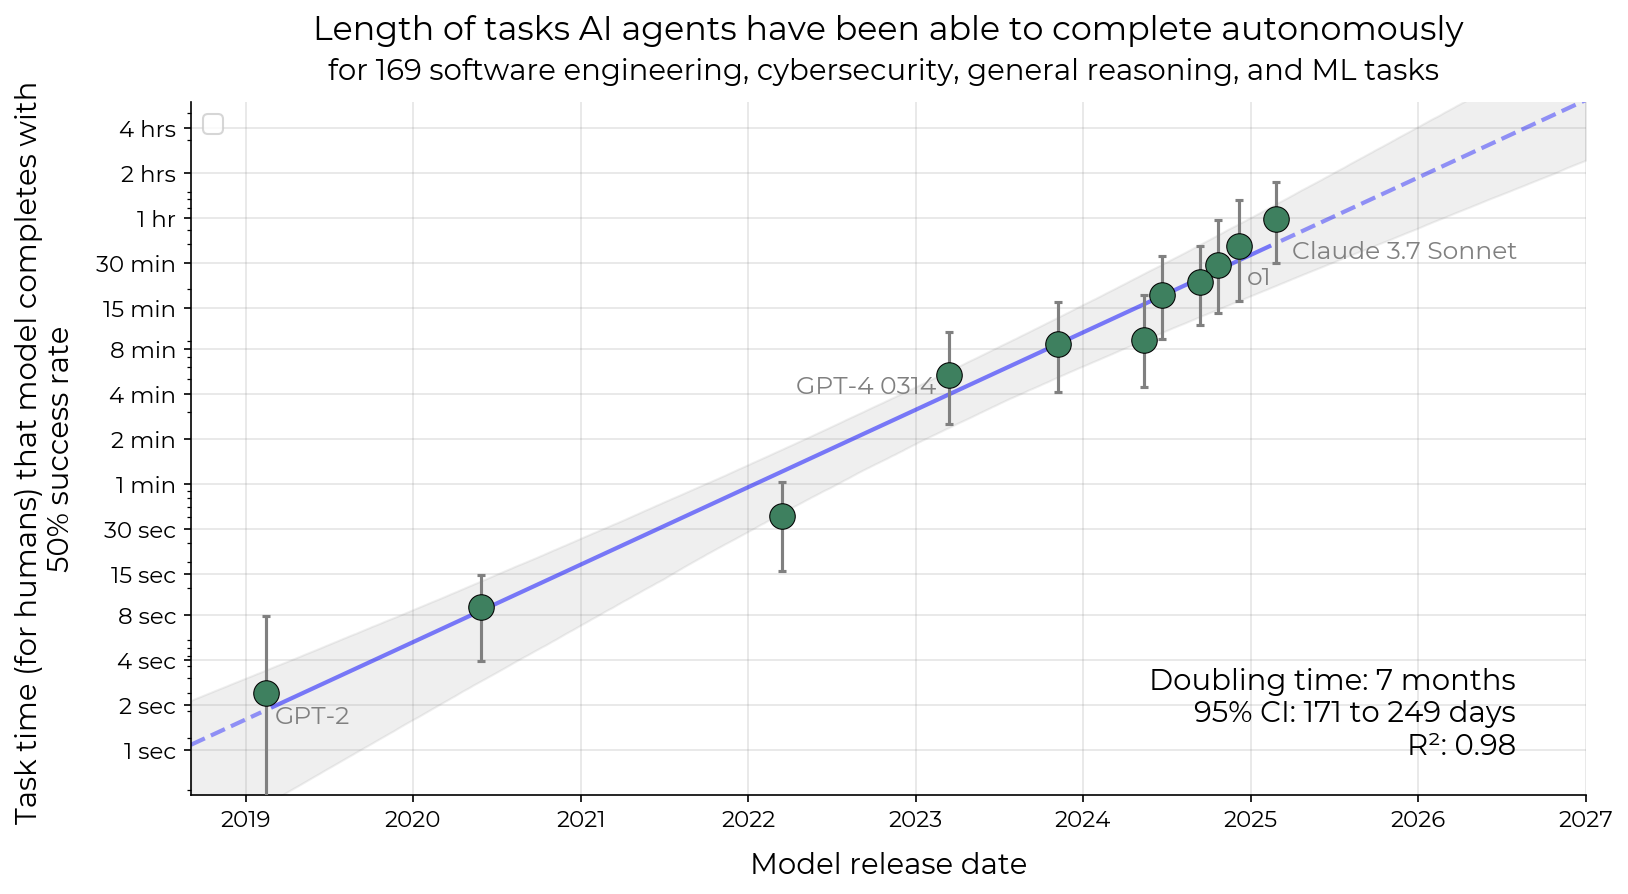
\includegraphics[width=0.9\linewidth]{plots_non_github/headline-green.png}
    \caption{The length of tasks (measured by how long they take human professionals) that generalist autonomous frontier model agents can complete with 50\% reliability has been doubling approximately every 7 months for the last 6 years (Section~\ref{sec:converting-to-horizon}).
    The shaded region represents 95\% CI calculated by hierarchical bootstrap over task families, tasks, and task attempts.
    Even if the absolute measurements are off by a factor of 10, the trend predicts that in under a decade we will see AI agents that can independently complete a large fraction of software tasks that currently take humans days or weeks (Section~\ref{sec:extrapolation}). 
    }
    \label{fig:headline}
\end{figure}



\setcounter{footnote}{0} % otherwise faisc link has footnote 5
In the last five years, frontier AI systems have undergone a dramatic transformation in capabilities, evolving from basic text generation \citep{radford2019language} to autonomously executing complex multi-hour machine learning research projects \citep{wijk2024re}. 
Sufficiently capable AIs could perform dangerous, highly complex actions like autonomous development of chemical, biological, radiological or nuclear weapons (CBRN) and self-replication and adaptation outside human control \cite{phuong2024evaluating}.
Understanding AI capabilities helps inform the development of safety guardrails as systems become increasingly powerful. 
In particular, many frontier AI developers have committed to using measures of specific AI capabilities to determine the necessary risk mitigations for their frontier AI systems.\footnote{An updated list of frontier AI safety policies can be found at: \url{https://metr.org/faisc}.} 
Robust benchmarks that can accurately track and forecast AI capabilities thus form the foundation for responsible
AI governance and risk mitigation. 

However, existing benchmarks face several key limitations. 
First, they often consist of artificial rather than economically valuable tasks. 
Second, benchmarks are often adversarially selected for tasks that current models struggle with compared to humans,\footnote{For example, HellaSwag \citep{zellers2019hellaswag} and Humanity's Last Exam \citep{phan2025humanity} were both generated by adversarially filtering problems against the best performing language models available at the time.} biasing the comparison to human performance. 
Most critically, individual benchmarks saturate increasingly quickly \citep{maslej2024aiindexreport}, and we lack a more general, intuitive, and quantitative way to compare between different benchmarks,\footnote{As with our tasks, SWE-bench Verified \cite{chowdhury2024SWEbench} does come with human-estimated task completion times. We use SWE-bench Verified tasks and accompanying time estimates to validate our main result in Section~\ref{sec:swebench}.} which prevents meaningful comparison between models of vastly different capabilities (e.g., GPT-2 versus o1). 
As a consequence, while the last few years have seen dramatic increases in AI performance on many individual benchmarks, understanding the progress of AI capabilities in general has required estimating the \emph{qualitative difficulty} of the latest benchmarks AI systems can pass. 

\begin{figure}
    \centering
    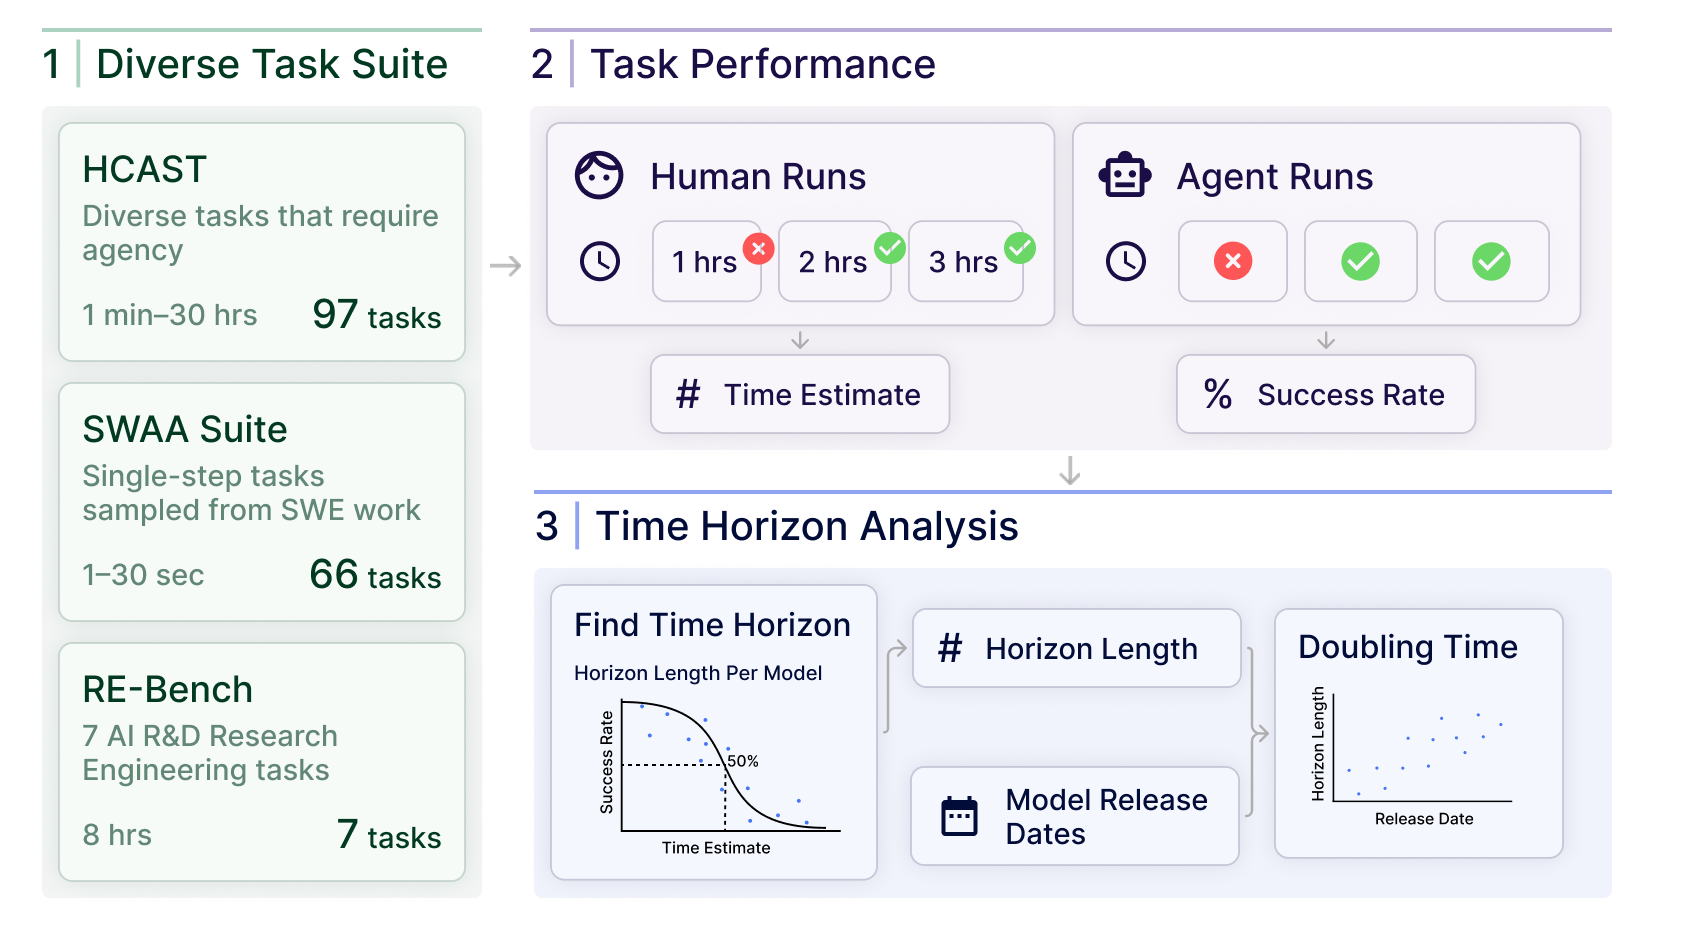
\includegraphics[width=0.9\linewidth]{images/methodology_new.png}
    \caption{Our methodology for measuring AI agent time horizon. First, we create a diverse task suite of \numtasks{} tasks. Second, we have both humans and AI agents (consisting of an AI model and a scaffold) attempt these tasks, recording the time taken by successful humans and the success rate for AI agents. Third, we fit a logistic model to find the time horizon at which each AI agent has a 50\% chance of success, and plot this against the release date of the model.}
    \label{fig:methodology}
\end{figure}

We propose tracking AI progress over time using the \textbf{task completion time horizon}: the duration of tasks that models can complete at a certain success probability, providing an intuitive measure of real-world capability compared to humans. 
As models may not reliably complete \emph{all} tasks of a given length, we operationalize this by measuring the \textbf{X\%-(task completion) time horizon}--the length of tasks that models can complete approximately X\% of the time.

% By comparing model performance against human baselines on \numtasks{} carefully designed software tasks spanning timescales from seconds to hours, we can track how the difficulty of tasks AI systems can handle has evolved over time. 
We prototype this methodology using three datasets designed to capture skills required for research or software engineering (Section~\ref{sec:tasks}), totaling \numtasks{} tasks with a wide range of difficulty: \gabenchmark{} \citep{METR_HCAST}, RE-Bench \cite{wijk2024re}, and Software Atomic Actions (SWAA), a new suite of shorter software tasks that can measure pre-2023 models (Section~\ref{sec:swaa}). 
Using skilled human baseliners, we estimate the duration that a domain knowledgeable human (without task-specific context) takes to complete these tasks (Section~\ref{sec:baselines}). 
We evaluate the performance of 13 frontier models from 2019 to 2025 on these tasks (Section~\ref{sec:model-performance}). Using methodology inspired by human psychometric studies, we then estimate the duration of tasks that models can complete with 50\% success rate---the 50\% time horizon (Section~\ref{sec:model_horizon_length}).

We find that the 50\% time horizon has been growing exponentially from 2019--2025 on our tasks, with a doubling time of approximately seven months (Figure~\ref{fig:headline}). We compare our main result with our exploratory results on non-SWAA tasks, finding that the 2023--2025 horizon growth rate is consistent with the 2019--2025 rate to within 11\% (Section \ref{sec:retrodiction}).
We also measure the 80\% time horizon of models (Figure~\ref{fig:p80}) and find a similar trend, though horizons are roughly 5x shorter. 
This progress appears to be driven by several key factors: improved logical reasoning capabilities, better tool use capabilities, and greater reliability and self-awareness in task execution (Section~\ref{sec:qualitative-analysis}).
\footnote{Code to reproduce our figures can be found at: \url{https://github.com/METR/eval-analysis-public}}
We also note several limitations of current systems---notably, performance is much lower on less structured, ``messier" tasks (Section~\ref{sec:messiness-split}). 

Since our tasks do not perfectly represent the average segment of intellectual labor by researchers and software engineers, this raises the question of external validity (Section~\ref{sec:externalvalidity}): whether the exponential trend holds on real-world tasks. We include results from three supplementary external validity experiments.


First, we score our \gabenchmark{} and RE-Bench tasks against a list of 16 ``messiness" factors that aim to capture some systematic differences between our tasks and hard``real-world" tasks. Some examples include whether the task is resource limited, novel, or involves a dynamic environment (Section~\ref{app:messiness}). Controlling for task length, we find models perform worse on tasks that have higher messiness scores. Notably, \textit{trends} in AI agent performance over time are similar for the lower and higher messiness subsets of our tasks (see Figure \ref{fig:2x2}). In particular, we find no evidence of plateaus in performance trends specific to our higher messiness subset. 

Second, we replicate our methods on SWE-bench Verified (Section~\ref{sec:swebench}), which includes human difficulty annotations. 
We find that the exponential trend still holds (Figure~\ref{fig:swebench}), albeit with an even shorter doubling time, possibly because SWE-bench Verified difficulty annotations, meant to represent high-context maintainer time, may differentially underestimate how long human contractors take to perform easier SWE-bench tasks.

Third, we measure AI agent performance on a small set of our internal pull requests (PRs) (Section~\ref{internal-prs}). We find large differences in the speed at which different human groups complete the internal PR tasks, with contractors taking 5-18x longer to fix issues than repo maintainers. When using contractor (rather than maintainer) time-to-complete as a measure of task length, model time horizons derived from combined performance on SWAA, \gabenchmark{} and RE-Bench are compatible with AI agent performance on internal PRs.

Our supplementary experiments find little evidence of performance trends being slower on the somewhat more realistic tasks we tested, but do not rule out the possibility that trends are meaningfully slower on the distribution of tasks required to automate software engineer jobs. These experiments were designed to detect large trend differences and constant factor shifts in model performance. We also find evidence that AI agent time horizons can differ by a large factor depending on the task domain and reference human population.

We conclude by discussing implications for AI capabilities forecasting (Section~\ref{sec:discussion}). Naively extrapolating the trend in horizon length implies that AI will reach a time horizon of \textgreater 1 month (167 work hours) between late 2028 and early 2031 (Figure~\ref{fig:multiverse-boxplot}). However, extrapolation is affected by both external validity concerns and future changes in the growth rate. We discuss several possible factors that could either speed up or slow down the future trend in Section \ref{sec:predicting-future-trends}.

\section{Related work}

\subsection{Agent and capability benchmarks}
The evaluation of AI capabilities has evolved significantly from single-task benchmarks to complex, multi-step evaluations designed to assess agent-like behavior. While traditional benchmarks such as GLUE \citep{wang2018glue}, SuperGLUE \citep{wang2019superglue}, and MMLU \citep{hendrycks2020measuring} have provided valuable insights into language model performance, they primarily measure static knowledge rather than the dynamic problem-solving capabilities essential for real-world applications.
Recent work has developed more complex agent benchmarks. AgentBench \citep{liu2023agentbench} evaluates agents across diverse environments including web browsing, coding, and game playing. MLAgentBench \citep{huang2024mlagentbench} focuses specifically on machine learning research tasks, while ToolBench \citep{qin2023toolllm} assesses tool use capabilities. The recent ZeroBench \citep{roberts2025zerobench} involve difficult reasoning, but in the context of visual puzzles rather than economically valuable tasks. Other noteworthy benchmarks include GAIA \citep{mialon2024gaia}, which evaluates reasoning across multiple modalities, and BIG-bench \citep{srivastava2022beyond}, which contains hundreds of diverse tasks including many requiring multi-step reasoning.

Software engineering has emerged as a particularly informative domain for evaluating AI capabilities. HumanEval \citep{chen2021evaluating} and MBPP \citep{austin2021program} provide programming challenges of varying complexity, while more complex benchmarks like SWE-bench \citep{jimenez2024swebench} and APPS \citep{hendrycks2021measuring} test more sophisticated programming abilities. We use SWE-bench Verified \citep{chowdhury2024SWEbench}'s human time estimates for task completion in our work. RE-Bench \citep{wijk2024re}, which we incorporate in our dataset, evaluates models on complex research engineering tasks that may require hours of human effort and compares AI performance to human machine learning engineers. 

While these benchmarks provide valuable insights into specific capabilities, they often lack a unified metric that allows for tracking progress over time and comparing models of vastly different capabilities. Our time horizon approach aims to address this gap by providing a continuous metric that can be used to measure progress across different capability levels.

\subsection{Forecasting AI progress}
Quantitative forecasting of AI progress has employed various approaches, often starting with the observation that the compute used in AI training has increased dramatically over time. \citet{amodei2018ai} observed that AI training compute usage has been increasing exponentially, doubling approximately every 3.4 months between 2012 and 2018; \citet{EpochNotableModels2024} included more recent data as well as trends in training dataset size and energy usage. 

Other work has studied how AI performance has increased over time, relating benchmark performance to release date, compute usage, and other inputs. \citet{sevilla2022compute} found that compute usage growth rate increased at the start of the ``deep learning era'' in 2010, coinciding with increases in performance. More recently, \citet{owen2024predictable} and \citet{pimpale2025forecastingfrontierlanguagemodel} use compute and other metrics to forecast future benchmark performance. 

Several recent efforts have been made to contextualize AI benchmark performance. One such effort is the annual AI Index Report \citep{maslej2024aiindexreport}, which tracks performance across various benchmarks, including the date at which models achieved human-level performance. 
\citet{murray2025mapping} had cybersecurity experts relate AI performance on Cybench \citep{zhang2024cybench} to the ability to autonomously develop malware. \citet{phuong2024evaluating} commissioned professional forecasters to predict whether AI ranks amongst top public concerns by 2030, conditioned on benchmark performance. 
These efforts generally lack a unified, quantitative metric for cross-benchmark comparison.

\citet{carlsmith2020compute} and \citet{cotra2020forecasting} developed the ``bio-anchors" framework, in which they related the compute involved in training AI models to the ``effective horizon length" of tasks required for AI to have transformative impacts. \citet{ngo2023tagi} proposed using the time horizon for which AI systems outperform most human experts at most tasks to measure general AI capabilities. In our work, we empirically evaluate the relationship between task duration and AI agent success rate, which we convert into a quantitative metric of AI agent performance.


\subsection{Psychometric methods and Item Response Theory}
Our methodological approach draws inspiration from psychometric testing, particularly Item Response Theory (IRT) \citep{baker2001basics}, which models the relationship between latent traits (such as ability) and observed responses to test items. In traditional IRT, item difficulty is a parameter in a logistic model predicting response correctness based on respondent ability. Our approach inverts this, using task completion time (a proxy for difficulty) to predict AI performance.
Our methodology also relates to difficulty estimation techniques in educational testing \citep{de2017handbook}, where multiple metrics including completion time are used to estimate the difficulty of tasks. IRT has been applied to machine learning classifiers by \citet{martinezplumed201918item}, and was used to design efficient benchmarks in \citet{song2021efficient}. 

\section{Measuring AI agent performance on realistic tasks} \label{methodology}



% \subsection{Overview}
\subsection{Task suite / dataset}\label{sec:tasks}

Our tasks are made up of three distinct task suites:

\begin{enumerate}

\item {A subset of \gabenchmark{} \cite{METR_HCAST}}: 97 diverse software tasks ranging from 1 minute to around 30 hours.\footnote{Our results also include one task from GAIA \citep{mialon2024gaia}, and five tasks involving writing code that is robust to an adversary, which are not included in \gabenchmark{}.}
\item RE-Bench \cite{wijk2024re}: 7 difficult ML research engineering tasks, all eight hours long.
\item Software atomic actions (SWAA): 66 single-step tasks representing short segments of work by software developers, ranging from 1 second to 30 seconds.
\end{enumerate}

All tasks are automatically scored with a continuous score or binary threshold; details of how we normalize and process scores are given in Section \ref{sec:model_horizon_length}. As with most benchmarks, our three task suites were also designed to isolate a specific unit of work that can be reliably accomplished within a time limit. This usually means that the tasks require much less context than the average task in the middle of a larger project.\footnote{We define context as information that experienced employees use to complete a task which is \textit{not} explicitly in the task description or possessed by most external experts. For example, when fixing a bug in a software package, the package's maintainer may use their experience with past bugs in the same package to guess at the bug's cause, fluency with the codebase to find the bug, and knowledge of their organization's priorities to decide whether to apply a quick patch or a more thorough fix. We discuss possible effects of context in Section~\ref{sec:externalvalidity}.} We confirmed that all tasks were doable given the instructions provided by having humans successfully complete each of our tasks at least once.\footnote{As many of these attempts were done by in-house staff or were done using different methodology, we exclude these attempts from our human baseline numbers.}

The \gabenchmark{} and SWAA suites are divided into \textit{task families}, which are groups of tasks that are similar. For example, the ``crossword" task family consists of tasks such as creating a 3x3 crossword puzzle, or a 5x5 crossword puzzle, etc. We segment tasks into families because performance within families is correlated and we down-weight families with many tasks for diversity.

\subsubsection{\gabenchmark{} tasks}

We use 97 tasks from 46 task families in \gabenchmark{}, a diverse set of challenges in cybersecurity, machine learning, software engineering, and general reasoning.

Tasks in this suite range from easy tasks that take humans a couple of minutes (e.g. looking up a basic factual question on Wikipedia) to tasks that take expert humans multiple hours (e.g. writing CUDA kernels, or fixing a subtle bug in PyTorch). Because modern frontier AI systems are relatively more proficient at text-based tasks, the majority of these tasks do not require visual/multimodal capabilities, and all tasks are solvable by text editing via a bash shell. 

Compared to many recent benchmarks, tasks in \gabenchmark{} are not designed to be as difficult as possible for either human domain professionals or current AI systems. Instead, most tasks are designed to be realistic, such that doing well on the task requires skills we expect to be economically useful. As a result, we expect that most of these tasks are solvable by humans with a few years of professional experience in the relevant domain. 

Tasks are defined by their instructions, starter resources, and an algorithmic scoring function. Task instructions are strings, typically between 1-2 sentences and a few paragraphs, although they can refer to other sources of information included as starter resources, or externally available via the internet. Starter resources typically consist of code, data, and documentation.

Each task is automatically scored between 0 and 1, with higher scores indicating better performance. Many tasks only return scores of 0 or 1, but for tasks with continuous scoring, we manually define a success threshold score, which we use in some of our analysis to binarize agent scores.\footnote{A small subset of these tasks {is publicly available} at \url{https://github.com/METR/public-tasks}. 
(We do not share the content of most tasks to reduce the likelihood of AI systems accidentally or intentionally being trained on them.)}

\subsubsection{RE-Bench suite}
RE-Bench consists of 7 challenging open-ended ML research engineering environments, each of which are intended to take a human expert approximately 8 hours to complete. See \citet{wijk2024re} for more details. 
% The tasks are listed in Figure \ref{fig:rebench}. 

\subsubsection{Software atomic actions (SWAA) suite}\label{sec:swaa}
\gabenchmark{} is designed to be a diverse set of tasks, but the shortest tasks are around 1 minute long, limiting both the representativeness and the achievable resolution in measuring AI agent performance on shorter tasks. To fill this gap, we observed that real-world intellectual labor consists in part of measurable, single-step actions shorter than 1 minute. We created the SWAA task suite, which comprises 66 small tasks corresponding to \textless1 minute atomic actions commonly performed in software engineering work. The SWAA subset includes both multiple-choice and completion questions. 

\begin{taskprompt}[Example SWAA task (file selection)]{1.0\textwidth}{0pt}
Which file is most likely to have a password in it?
    1. credentials.txt
    2. installation_notes.txt
    3. main.py
    4. launcher_win.exe
\end{taskprompt}

In contrast to other simple benchmarks like LAMBADA \citep{paperno2016lambada} or GSM8K \citep{cobbe2021training}, which test skills not directly applicable to software engineering, the SWAA set represents actions that are needed in both software engineering work and our longer tasks. SWAA consists of 5 task families, three representing common decisions, one for code completion, and one for math; see Appendix \ref{sec:appendix-swaa} for more details.

Development of SWAA tasks was blind to AI agent performance; that is, all tasks were written before seeing AI attempts, and elicitation (development of the few-shot prompt used for evaluation) was carried out on a separate development task suite.

\subsubsection{Examples of tasks of varying lengths}
Table \ref{tab:task_family_summaries}  contains example tasks. Tasks that take less than one minute measure knowledge which would be needed for professional software engineering but do not require agency. At around one minute, tasks become similar to components of economically valuable work but are not entire projects (e.g. answering a basic question on Wikipedia). At about ten minutes, tasks become the difficulty of approximately the easiest meaningful step of a real software project (e.g. configuring a common open-source package). The shortest tasks which could reasonably be said to be standalone economically valuable projects take around one hour (e.g. writing a script to transform data from one format into another) and by eight hours tasks represent meaningfully valuable software projects (e.g. speeding up a python script by implementing custom CUDA kernels). Many more examples of these tasks are provided in \citet{wijk2024re} and \citet{METR_HCAST}.

\begin{table}[]
    \centering
    \begin{tabular}{p{0.2\linewidth}p{0.15\linewidth}p{0.55\linewidth}}
    \hline
\textbf{Family} &\textbf{Length} & \textbf{Description} \\
\hline
find\_shell\_script & 3 seconds & Multiple choice: ``Which file is a shell script?"
    Choices: ``run.sh", ``run.txt", ``run.py", ``run.md" \\
\hline
wikipedia\_research & 1 minute & Research simple factual information from Wikipedia and provide accurate
answers to straightforward questions. \\
\hline
         oxdna\_simple & 9 minutes & Detect and fix a bug in the input files for a molecular dynamics simulation using the oxDNA package. \\
\hline
munge\_data & 56 minutes & Write a Python script to transform JSON data from one format to another by inferring the conversion rules from provided example files. \\
\hline
cuda\_backtesting & 8 hours & Speed up a Python backtesting tool for trade executions by implementing custom CUDA kernels while preserving all functionality, aiming for a 30x performance improvement. \\
\hline
    \end{tabular}
    \caption{Example tasks of differing durations. More examples can be found in \citet{METR_HCAST} and \citet{wijk2024re}.}
\label{tab:task_family_summaries}
\end{table}

\subsection{Baselining}\label{sec:baselines}
In order to ground AI agent performance, we also measure the performance of multiple human ``baseliners'' on most of our tasks and recorded the duration of their attempts. 
In total, we use over 800 baselines totaling \baselinehours{} hours, of which \numbaselines{} baselines (\numsuccessfulbaselines{} successful) come from \gabenchmark{} and RE-Bench, and 249 (\numswaabaselines{} successful) from the shorter SWAA tasks.

\paragraph{Baseliner skill and experience} Our baseliners are skilled professionals in software engineering, machine learning, and cybersecurity, with the majority having attended world top-100 universities. They have an average of about 5 years of relevant experience, with software engineering baseliners having more experience than ML or cybersecurity baseliners.

\subsubsection{\gabenchmark{} tasks}

We use existing baselines collected as part of \gabenchmark{}. These baselines are collected from domain professionals with relevant experience in software engineering, ML, and cybersecurity. Baseliners work in the same environment as agents, using Vivaria,\footnote{Our open source platform for language model agent evals: \url{https://vivaria.metr.org/}.} with their screens and audio recorded for manual review, to prevent cheating. They are incentivized with bonuses for successful completion and for completing tasks faster than other baseliners. After screening out failed attempts and those with issues (such as using disallowed AI tools), we use \numsuccessfulbaselines{} successful baselines from approximately 460 total attempts. Task durations are calculated using the geometric mean of successful baselines, with manual estimates for tasks lacking successful baselines.\footnote{Non-baseline estimates were based on information including the length of QA runs that did not follow strict baseline conditions, and the length of similar tasks with successful baselines.}

\subsubsection{RE-Bench}
For RE-Bench, we used the baselines from the RE-Bench paper. As baseliners were instructed to achieve the best performance for each task, we consider the task duration of each of these 6 tasks as 8 hours, and instead use the mean score achieved by baseliners who spent between 7 and 9 hours to convert raw score into success threshold. 

\subsubsection{SWAA}
Unlike \gabenchmark{} and RE-Bench, which were baselined by external contractors, SWAA is baselined by METR employees with relevant expertise using a custom webapp that enables more accurate timing. Because these tasks are intended to be a single step and exclude context acquisition, the timer for SWAA tasks ends as soon as the user chooses a response. For decision based tasks, only one selection is allowed to avoid random guessing; for fill in the blank tasks, baseliners can try multiple times until getting the answer correctly or opting to skip. We baselined each decision-based task 4 times and each fill-in-the-blank style task 3 times. 

\begin{table}[t]
\centering
\begin{tabular}{lcc}
\hline
\textbf{Suite} &\textbf{Time Estimate Source} & \textbf{Number of Tasks} \\
\hline
\gabenchmark{} & Estimate & 21 \\
 & Baseline & 76 \\
\hline
RE-Bench & Estimate & 0 \\
 & Baseline & 7 \\
\hline
SWAA & Estimate & 0 \\
 & Baseline & 66 \\
\hline\\
\end{tabular}
\label{tab:estimate_sources}
\caption{The source of our time estimates by task suite. In total, 148 of our 169 tasks have human baselines, but we rely on researcher estimates for 21 tasks in \gabenchmark{}.}
\end{table}


\subsection{Evaluating AI agent performance on task suites}\label{sec:model-performance}
Most models we evaluated in this paper were models we had previously evaluated and therefore could reuse our scaffolding. We also included the earlier frontier models gpt-3.5-turbo-instruct, davinci-002 (GPT-3), and GPT-2. Full information on the models and agents used can be found in Appendix~\ref{app:how-run}.

\subsubsection{Agent scaffolds}
We used the same agent scaffolds across the evaluation suite, with no task-specific prompting or scaffolding, except for the SWAA tasks, which used a simple prompting scaffold. All agents were provided with the same affordances provided to human baseliners. 

Most AI models were evaluated with {modular-public}---our basic agent scaffold.\footnote{Code for this agent scaffold can be found at \url{https://github.com/poking-agents/modular-public}.} This scaffold provides the model with Python and Bash commands and some very simple context management to keep the input within the context window length of the LM. We used a slightly different scaffold for o1-preview and o1, because they seemed to struggle with tool use, responding to environmental feedback, and generally acting as an agent. These are described further in Appendix \ref{app:how-run}. 

GPT-2 is incompatible with our scaffolding due to low context length, so we imputed a score of zero for GPT-2 on all tasks in RE-Bench and \gabenchmark{}. We think this is reasonable because the far more capable davinci-002 (GPT-3) scores zero on this set. Removing these imputed GPT-2 zero scores has a negligible effect on all subsequent results in this paper. 

\begin{figure}
    \centering
    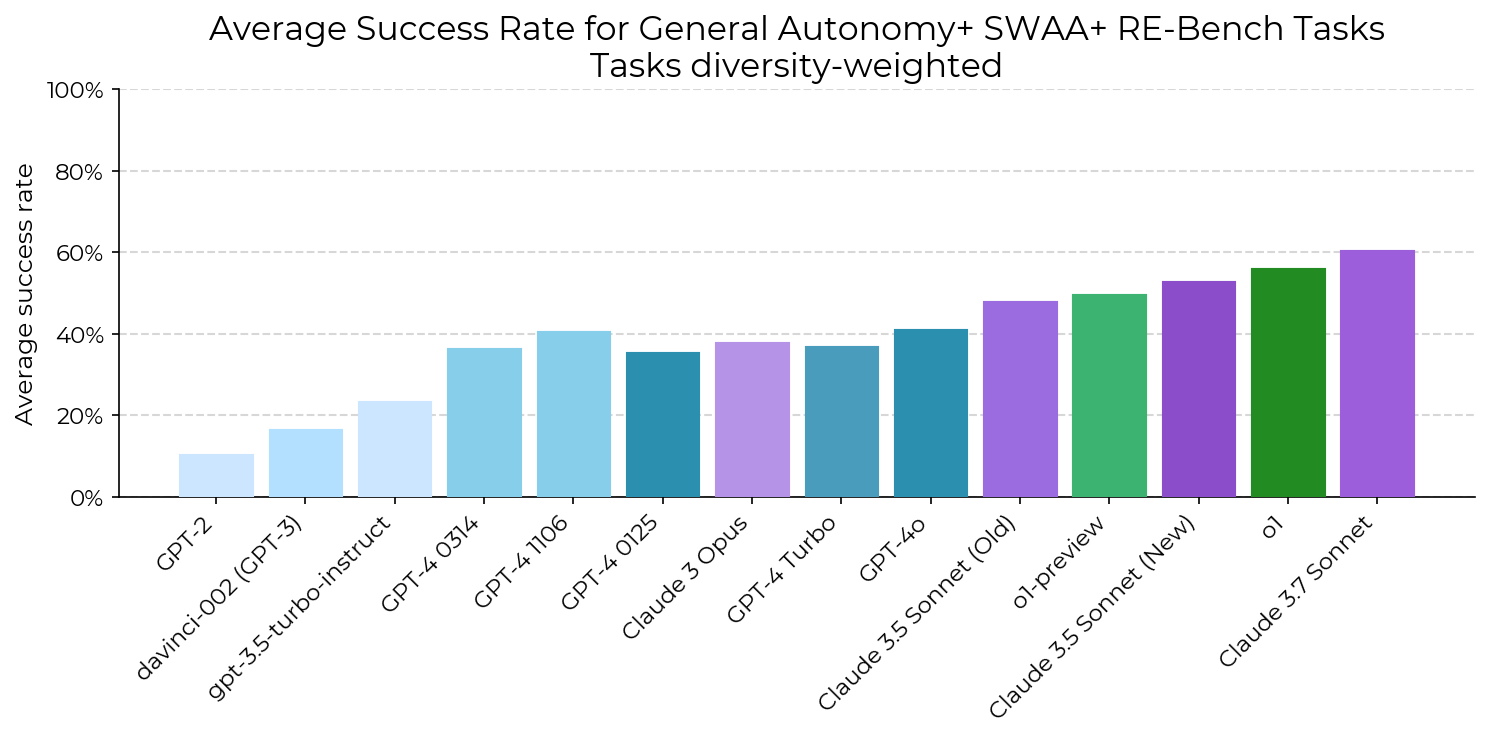
\includegraphics[width=0.8\linewidth]{plots/bar_chart_weighted_scores/headline.png}
    \caption{Average task success rate across our entire combined suite, for each model. As with all of the results reported in the main body of this work, to reduce the influence of large task families, we weight each task by the inverse square root of the number of tasks in the family it belongs to.}
    \label{fig:scores}

\end{figure}

\subsubsection{Results}
We performed 8 runs\footnote{This number is approximate, because a small number of runs failed due to internal infrastructure issues.} per agent/task pair and report the average results in Figure~\ref{fig:scores}. As with most benchmarks, we notice a strong upwards trend over time, with recent models completing approximately 50\% of all tasks, while earlier models perform substantially worse. We note that there is substantial correlation between the tasks that models can complete (Figure~\ref{fig:corr_matrix_observed_success_rates}), with average correlation of approximately 0.73. 


\subsubsection{Model success rate vs baseline time}

There is a negative correlation between the time it takes a human baseliner to complete a task and the average success rate (across all models) on the task. This decrease in success rate over length (Figure \ref{fig:success_vs_time}) is well-fit by an exponential model ($R^2 \approx 0.83$ when regressing model success rate against the logarithm of human time-to-complete). Notably, the correlation of model success with log human time (0.91) is higher than the average correlation between models (0.73, see Figure \ref{fig:corr_matrix_observed_success_rates}). 

We sanity check this fit by examining the human-time-to-complete of tasks that earlier versus later models can complete. As expected, pre-2023 models like GPT-2 or GPT-3 can complete tasks requiring only writing a few words, but fail all tasks above 1 minute. In contrast, recent frontier models such as Claude 3.5 Sonnet (new) and o1 can complete some tasks that take human baseliners more than 4 hours (Figure~\ref{fig:hist}). 



\section{Computing time horizon} \label{sec:converting-to-horizon}
To calculate a more intuitive metric for AI capabilities progress, we convert the performance of each model on our tasks to an estimate of their task completion time horizons. 

\subsection{From raw data to time horizon} \label{sec:model_horizon_length}

First, the agent performance on each task is converted to a binary value (success or failure).  Many tasks are naturally binary, including all SWAA tasks and the majority of \gabenchmark{} tasks. Some tasks are continuously scored; these are binarized via a task-specific threshold. For example, if the task is to minimize the loss of a model, runs are binarized based on whether they achieved a loss below some threshold. Note that binarization particularly affects more challenging tasks such as RE-Bench, since current frontier models' partial progress is usually binarized to 0 (as they are below human level on these tasks).

% For side by side plot use plots/success_rate_scatter_and_logistic/headline.png and set width to 0.8\linewidth
\begin{figure}
    \centering
    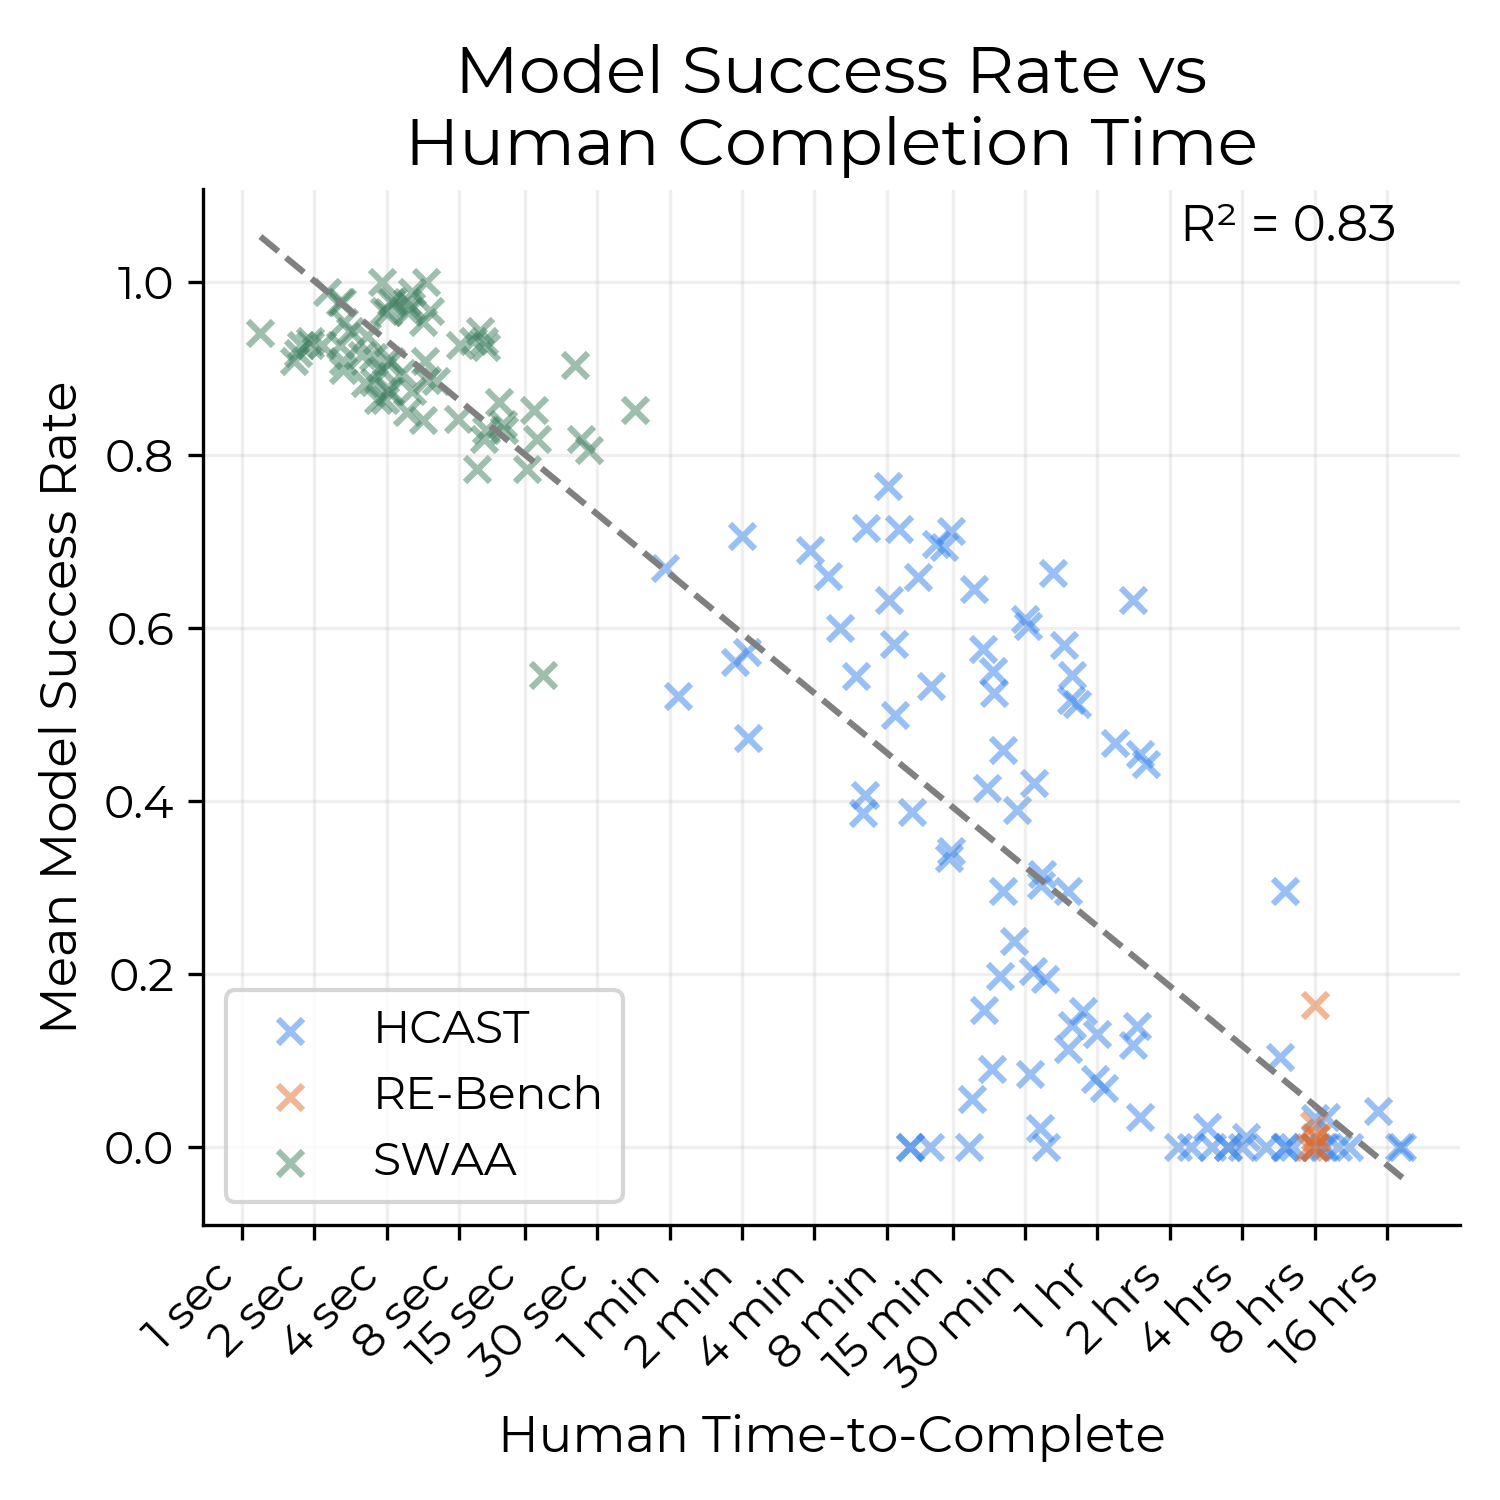
\includegraphics[width=0.5\linewidth]{plots/success_rates/model_success_rate_vs_human_completion_time.png}
    \caption{Model success rates are negatively correlated with how much time it takes a human to complete the task. ($y=-0.07x+0.66$, $R^2: 0.83$)}
    \label{fig:success_vs_time}
\end{figure}

\begin{figure}
    \centering
    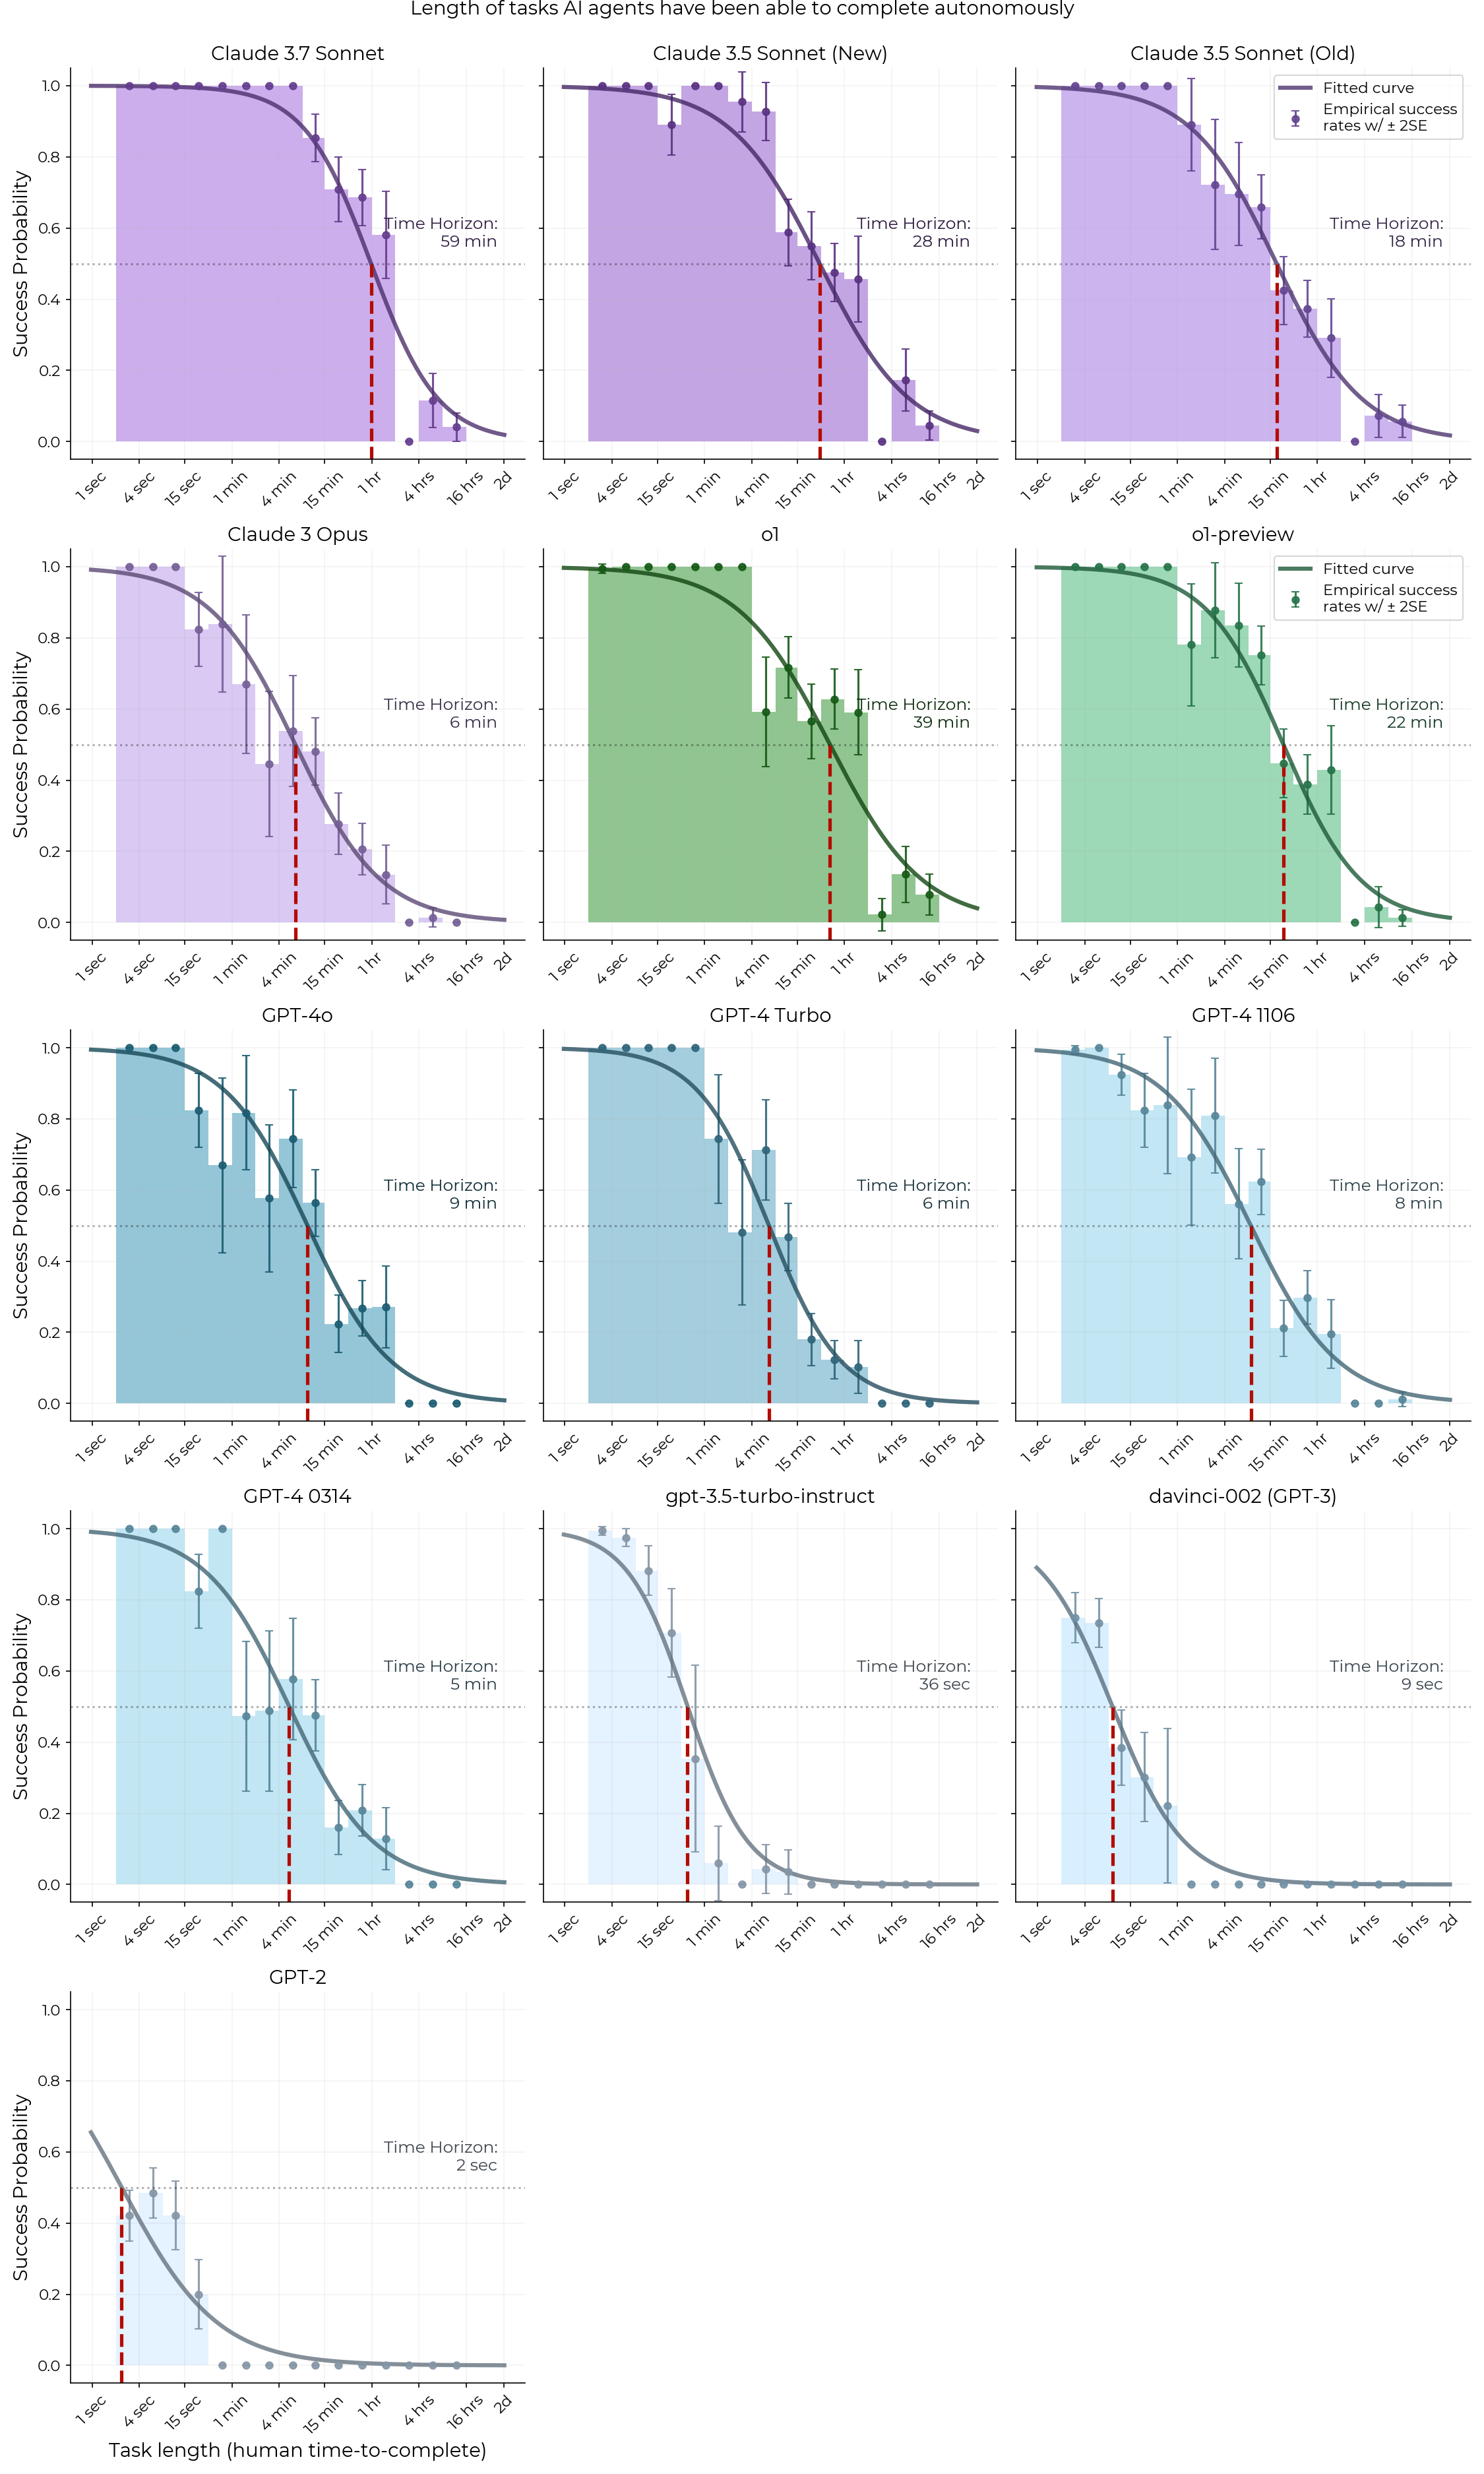
\includegraphics[width=0.9\linewidth]{plots/individual_histograms/default/histograms.png}
    \caption{Success rates of all models on our test suite, showing the computation of time horizon as predicted 50\% success rate time. The logistic fit is fairly good, though there is a jump in success rate between \textless 1 minute tasks and \textgreater 1 minute tasks, which corresponds to the boundary between SWAA and \gabenchmark{} tasks.}
    \label{fig:hist}
\end{figure}

The task-specific threshold is chosen to represent human performance. For \gabenchmark{}, the task-specific threshold is the same ``target score" the human baseliner tries to achieve, which we also use to filter for successful runs. RE-Bench tasks have a fixed time rating of 8 hours, so the task-specific threshold is the average score of 7-9--hour human runs.

Once we have agent success rates and time ratings for each task, our approach is inspired by item response theory (IRT) \cite{baker2001basics}. Like in IRT, we use logistic regression to find the task difficulty at which the agent has a 50\% chance of success, but unlike IRT, we exploit the fact that we have human baselines to use difficulty ratings based on human time rather than ratings learned from agent performance. Specifically, we perform logistic regression using:

\[
p_{\mathrm{success}}(\mathrm{model}, \mathrm{task}) = \sigma((\log h_{\mathrm{model}} - \log t_\mathrm{task}) \cdot \beta_\mathrm{model})
\]

where $t_\mathrm{task}$ is the geometric mean time of successful human baselines, and $h_\mathrm{model}$ and $\beta_\mathrm{model}$ are learned parameters, with $h_\mathrm{model}$ representing the 50\% horizon time. Further details and comparison to standard IRT methods are provided in Appendix \ref{app:irt}.

\paragraph{Excess success rates}
Excess success rates ($\frac{S_{observed}-S_{predicted}}{S_{predicted}}$)
are a metric for how much better (or worse) an AI agent performed compared to what we would expect, given a task's length and that model's ability (expected success can be seen in Figure \ref{fig:hist}). The average correlation between model excess success rates across all tasks is 0.40, indicating that AI agents still have moderately correlated performance when controlling for task length (See Figure \ref{fig:corr_matrix_fractional_success_rates} for the full correlation matrix).

\subsection{Model horizon length vs. release date}

In Figure~\ref{fig:headline}, we plot the time horizons of each model against their release date---the date at which the lab first publicly announced the frontier model.\footnote{In most cases, the release date is for each frontier AI model is the same model as the one we evaluated. However, GPT-3 (davinci) and GPT-3.5 (code-davinci-002 and text-davinci-002) are closed-source and no longer available through API access, but we use their release dates for the closest available models, which OpenAI advertises as having equivalent performance: GPT-3's release date for davinci-002, and GPT-3.5's date for gpt3.5-turbo-instruct.} In addition, we linearly regress\footnote{Specifically, we perform Ordinary Least Squares regression on $\log(\text{model\_horizon}) = \alpha + \beta \cdot  \text{release\_date}$. In Appendix \ref{app:robustness} we discuss other curve-fitting methods, and conclude that the fit is not sensitive to various hyperparameters such as regularization, weighting of tasks, or WLS vs. OLS.} $\log(\text{time horizon})$ against release date, finding that time horizon has doubled every 212 days with a 95\% bootstraped confidence interval 171--249 days (or $\pm 19\%$). Error bars are calculated via \nbootstrap{} samples from a three-level hierarchical bootstrap over task families, then tasks, then runs. 

While there are wide error bars on each individual models' horizon lengths, these errors are highly correlated between models. This is because tasks at the same human time rating vary widely in difficulty for models, and sampling easy (or hard) tasks will result in a higher (or lower) horizon estimate for all models. Therefore, we are more confident in the slope of the time horizon trend than in the time horizon of any particular model. The fit is not sensitive to various hyperparameters such as regularization, weighting of tasks, and WLS vs. OLS (see Figure \ref{fig:multiverse-boxplot}). 

Horizon length on our tasks increases substantially over the entire time period from 2019 to early 2025. Base models like GPT-3 can complete some tasks requiring only writing a few words, but fail all tasks above 1 minute. Chat models like GPT-4 and Claude 3 Opus are able to complete the easier \gabenchmark{} tasks with some frequency, leading to time horizons in the 5--30 minute range. However, the trend in 2024 and early 2025 may be faster, with o1 and Claude 3.7 Sonnet lying above the long-run trend. Though the gap is difficult to distinguish from noise, it is robust to methodological ablations like using continuous scoring (Appendix~\ref{app:robustness}).

\subsubsection{Time horizons at 50\% success rate vs 80\% success rate} \label{sec:p80}

\begin{figure}
    \centering
    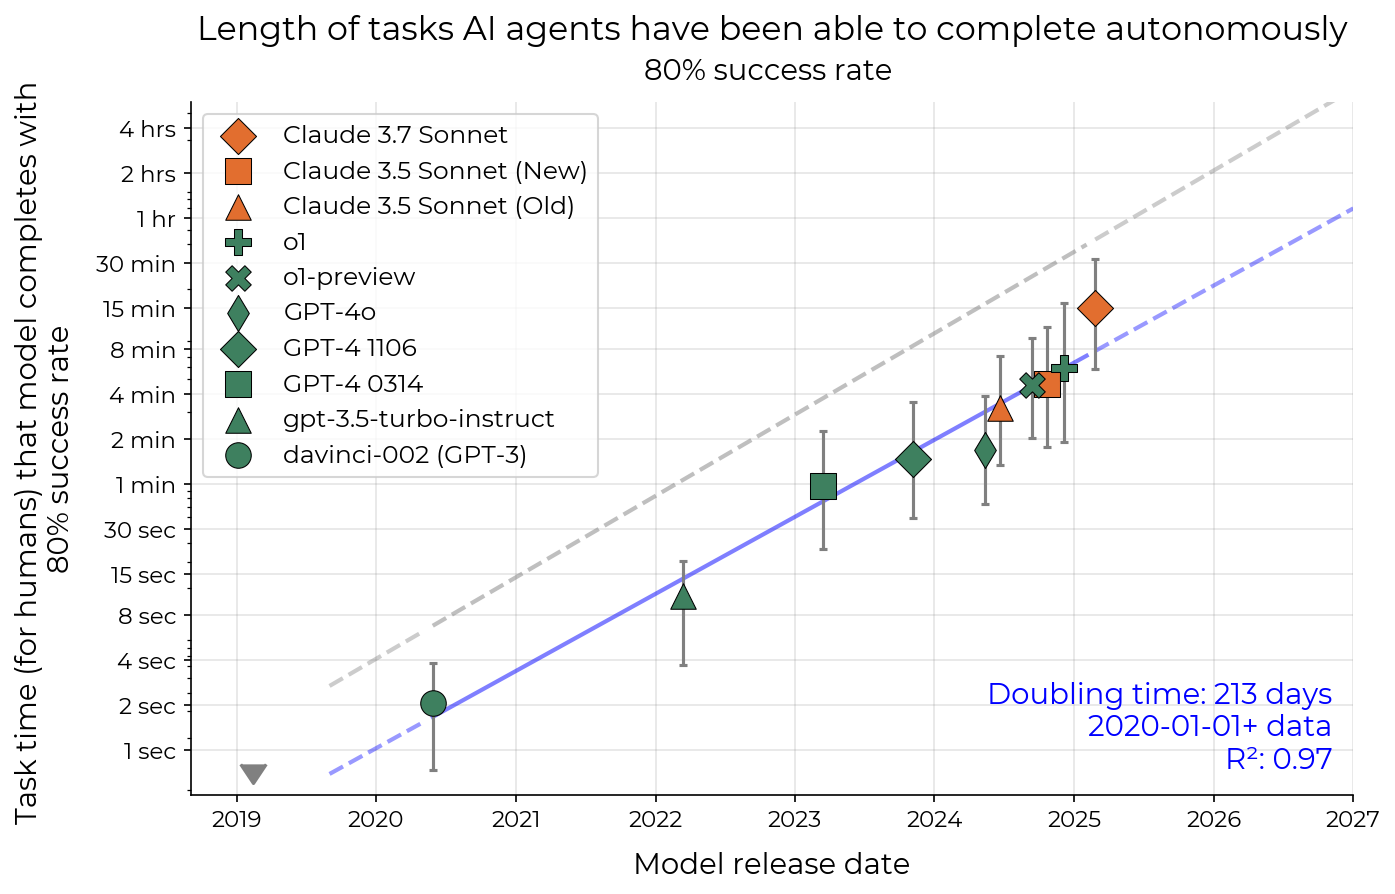
\includegraphics[width=0.8\linewidth]{plots/logistic/p80.png}
    \caption{Trend in 80\% success rate time horizon. The doubling time is similar to the 50\% plot, but horizons are substantially lower. 50\% horizon trend shown in grey.}
    \label{fig:p80}
\end{figure}

To check whether our choice of 50\% success rate affects the long-run trend, we also compute the time horizon at which AI agents succeed at tasks with 80\% success rate, shown in Figure~\ref{fig:p80}. The doubling time in 80\% time horizon (213 days) is similar to the doubling time of 50\% time horizon (212 days), within margin of error. However, there is a large gap between models' 50\% time horizon and 80\% time horizon---Claude 3.7 Sonnet has the longest 80\%-horizon among models we examined at around 15 minutes, in contrast to its 50\%-horizon of 59 minutes. This gap suggests that even models that sometimes succeed on difficult and diverse tasks cannot reliably perform tasks of moderate length. Due to our limited dataset, we cannot confidently measure time horizons at very high success rates (e.g. 95\%)-- see Section~\ref{sec:measuring-extreme-time-horizons}.


\section{Qualitative analysis} \label{sec:qualitative-analysis}

To better contextualize the observed trend of improved model performance, we examined the transcripts for the tasks where earlier models (e.g. GPT-4) do substantially worse than current models. 
Specifically, we categorized our task families based on the type of expertise required, and noticed that current models tend to outperform earlier models for tasks that involved ML training, reverse engineering compiled software binaries, and cybersecurity CTFs. 
In addition, we noticed that agents improved greatly on tasks requiring situational awareness of the AI agent's limitations or defeating an opposing strategy. 
This gave us five sets of task families to examine.

For each of these task family sets, we then used contractors to manually read through all runs from all models for all tasks in each of these five task families, and identified possible explanations for the improvement in AI agent performance on those tasks, as well as potential limitations. We find that models seem to have improved greatly in terms of tool use capabilities, demonstrate a markedly greater ability to adapt to mistakes (as opposed to repeating unsuccessful actions), and perform much better at parts of tasks requiring logical reasoning or code generation. However, we noticed that AI agents still seem to struggle in intuitively ``messier" environments---specifically, environments without clear feedback loops, or where the agent needs to proactively seek out relevant information. We provide examples of both the improvements and these limitations in Appendix~\ref{sec:more-qualitative-analysis}.

To better understand the differences between current and older AI agent failures, we separately sampled 31 unsuccessful agent runs from our GPT-4 1106 agent and 32 unsuccessful runs from our o1 agent, and manually labeled them for the following exclusive categories of failures:
\begin{itemize}
    \item \textbf{Poor planning and tool choice}: the agent generates a high level plan that seems unworkable on its own merits, or picks tools for the plan that would not accomplish the desired purpose. 
    \item \textbf{Incorrect mental math or reasoning}: the agent performs incorrect mental math or logical reasoning at a crucial step, causing the run to fail. 
    \item \textbf{Premature task abandonment}: The agent abandons the task in the middle of the attempt and either submits a nonsensical answer or submits a solution without checking for correctness. These failures often result from the agent submitting their answer before looking at all the pieces of code or information required to arrive at the correct solution. 
    \item \textbf{Repeating failed actions}: The agent repeats the same behavior that doesn’t make progress toward the problem, such as running a command that leads to an error over and over again, without trying other approaches.
\end{itemize}
We report the results in Table~\ref{tab:failure-comparison}. We find that over a third of the GPT-4 failures resulted from repeating failed actions, compared to 2 out of 32 for o1, which we see as quantitative evidence for our claim that models seem to have improved in their ability to adapt to mistakes. Interestingly, half of the o1 failures resulted from abandoning the task prematurely, while only a quarter of the GPT-4 failures resulted from the same---this may result from o1 failures occurring on qualitatively more difficult tasks, or may reflect idiosyncrasies of o1. 

% from: https://docs.google.com/spreadsheets/d/1b-LJ1nvPwgyzAzVLI-f2HH0UTIrYU0D8BrpOPUvP2Uk/edit?gid=505028176#gid=505028176
\begin{table}[t]
    \centering
    \begin{tabular}{lcc}
        \hline
        \textit{Failure type} & GPT-4 1106 & o1 \\
        \hline
        Poor planning/tool choice & 4 & 6 \\
        Incorrect mental math/reasoning & 6 & 7 \\
        Premature task abandonment& 8 & 16\\
        Repeating failed actions & 12 & 2\\
        Other & 1 & 1\\
        \hline
        Total & 31 & 32\\
        \hline \\
    \end{tabular}
    \caption{Number of different categories of failures for 31 failed runs by GPT-4 1106 and 32 failed runs by o1 (Section~\ref{sec:qualitative-analysis}). Note that as o1 succeeds at more tasks, its failures correspond to more challenging tasks compared to GPT-4's failures.}
    \label{tab:failure-comparison}
\end{table}

\section{External validity and robustness} \label{sec:externalvalidity}

To investigate the applicability of our results to other benchmarks, and to real task distributions, we performed four supplementary experiments. 
First, we check whether the 2023--2025 trend without the SWAA dataset retrodicts the trend since 2019, and find that the trends agree.
Second, we label each of our tasks on 16 ``messiness" factors---factors that we expect to (1) be representative of how real-world tasks may systematically differ from our tasks and (2) be relevant to AI agent performance.
Third, we calculate AI agent horizon lengths from SWE-bench Verified tasks. We find a similar exponential trend, although with a shorter doubling time. However, we believe this shorter doubling time to be a result of SWE-bench Verified time annotations differentially underestimating the difficulty easier SWE-bench tasks.
Finally, we collect and baseline a small set of uncontaminated issues from internal METR repositories. We find that our contracted human baseliners take much longer to complete these tasks than repository maintainers. We also find that AI agent performance is worse than would be predicted by maintainer time-to-complete but is consistent with contractor time-to-complete, given the AI agent success curves from \gabenchmark{} + SWAA + RE-Bench tasks shown in Figure \ref{fig:hist}. 

\begin{figure}
    \centering
    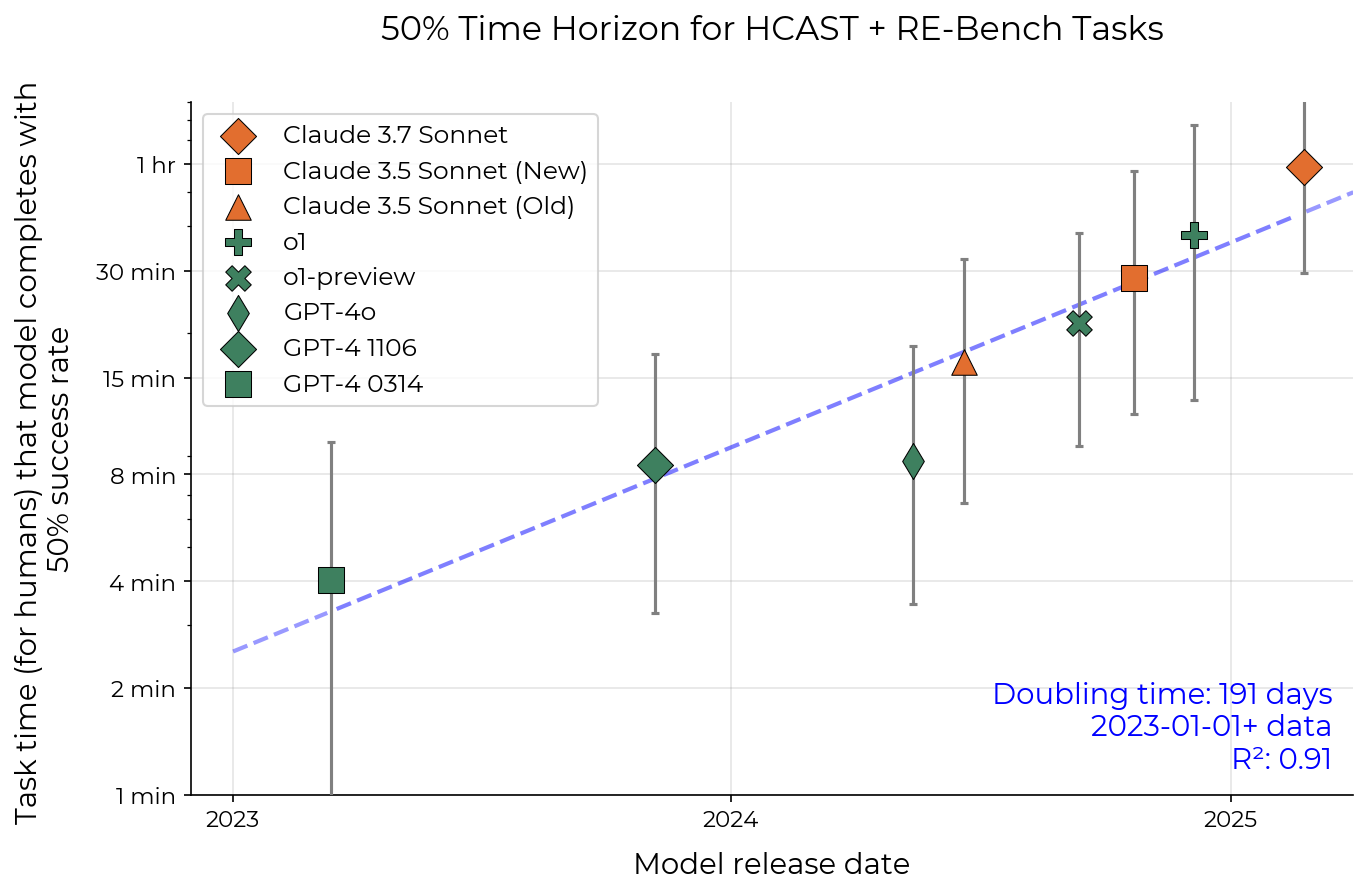
\includegraphics[width=0.8\linewidth]{plots/logistic/single_line_2023_ga_rebench.png}
    \caption{Time horizons on \gabenchmark{} + RE-bench, for models starting with GPT-4 0314.}
    \label{fig:2023}
\end{figure}

\subsection{Retrodiction from 2023--2025 data} \label{sec:retrodiction}


As part of exploratory work for this paper, we measured the time horizon of 9 frontier and near-frontier models released in 2023 and 2024, using only our \gabenchmark{} and RE-Bench suites. This trend (with Claude 3.7 Sonnet added) is shown in Figure~\ref{fig:2023}: time horizon doubles about every six months. Since we only had two 2023 models (GPT-4 0314 and GPT-4 1106) and a small data range (release date spanning 2 years and time horizon spanning 5 doublings), error bars were very wide. In addition, restricting our data further to 2024-only models produced a different trend with time horizon doubling about every three months, so any extrapolation into the future would not be robust.

To address these issues, we collected more data to extend the trendline into the past, developing the Software Atomic Actions (SWAA) suite to decrease the minimum human time of our task suite from 1 minute to under 2 seconds, and enabling us to measure GPT-2, davinci-002 (GPT-3) and GPT-3.5-turbo-instruct on the combined suite.

The 2023--2025 trend retrodicts the longer-term trend well (Figure~\ref{fig:retro}). The measured doubling time over the whole 6 year period 2019--2025 inclusive was 212 days, which closely matches the 191-day trend based on data from non-SWAA tasks and 2023--2025 models.

\begin{figure}
    \centering
    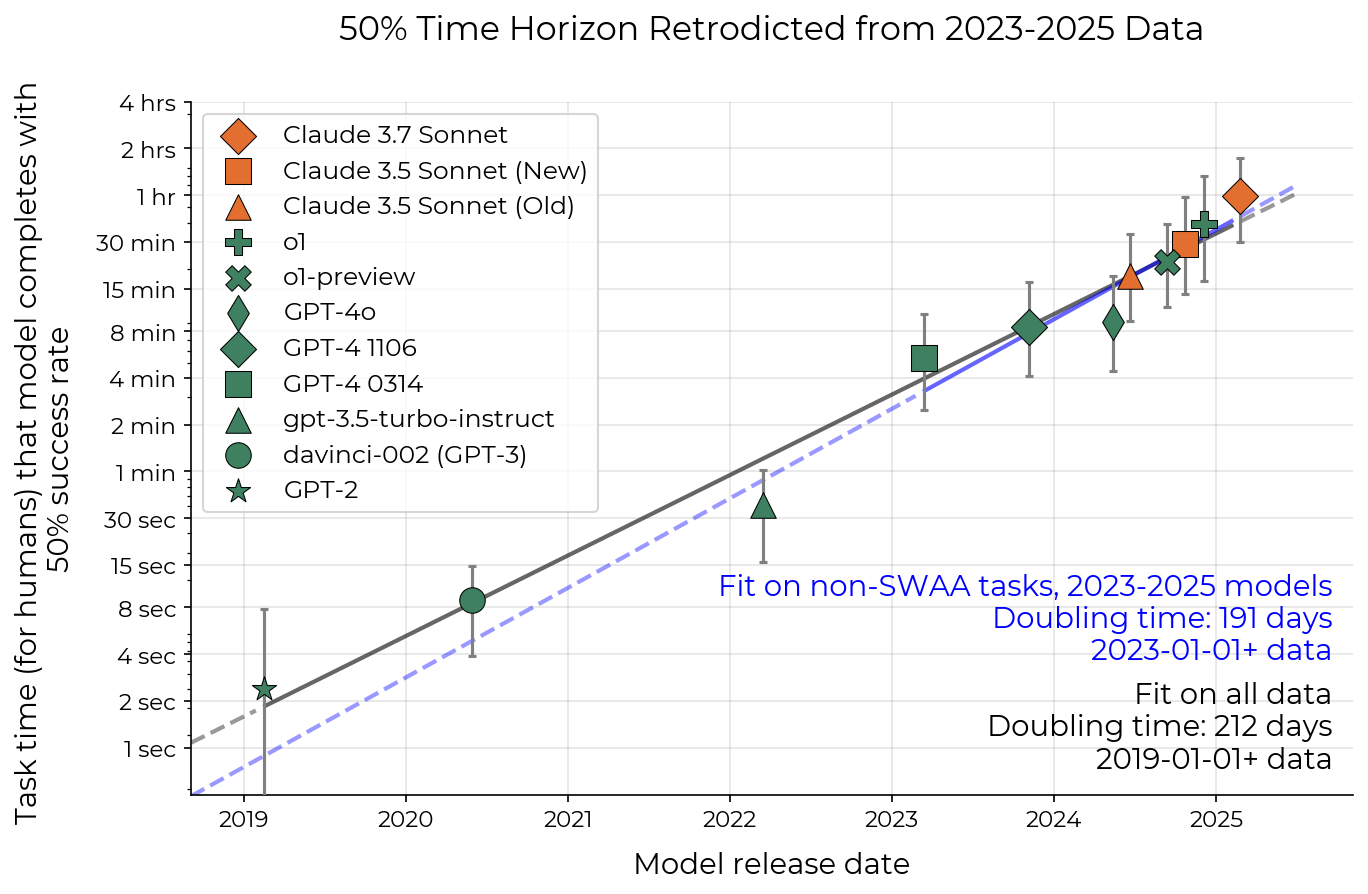
\includegraphics[width=0.8\linewidth]{plots/logistic/double_line_all_data_retrodict_excluding_swaa.png}
    \caption{The full time series for the time horizon of models, by release date. We plot in blue the regression from only 2023+ data on \gabenchmark{} + RE-Bench tasks, extended into the past, and in gray the regression with all tasks (including SWAA) on the whole 6 year period. Points on the graph are models' time horizons on all data including SWAA.}
    \label{fig:retro}
\end{figure}

\subsection{Messiness factors}\label{sec:messiness-split}

Real-world intellectual labor often involves messy details that benchmarks usually don't include, such as being under-specified or poorly scoped, having unclear feedback loops or success criteria, or requiring coordination between multiple streams of work in real-time. We generally observed that agents struggle more on tasks that have these ``messy" details (Section~\ref{sec:qualitative-analysis}). A natural question is therefore whether agents showed similar rates of improvement on ``less messy" and ``more messy'' tasks.

\begin{figure}
    \centering
    \vspace{-20pt}
    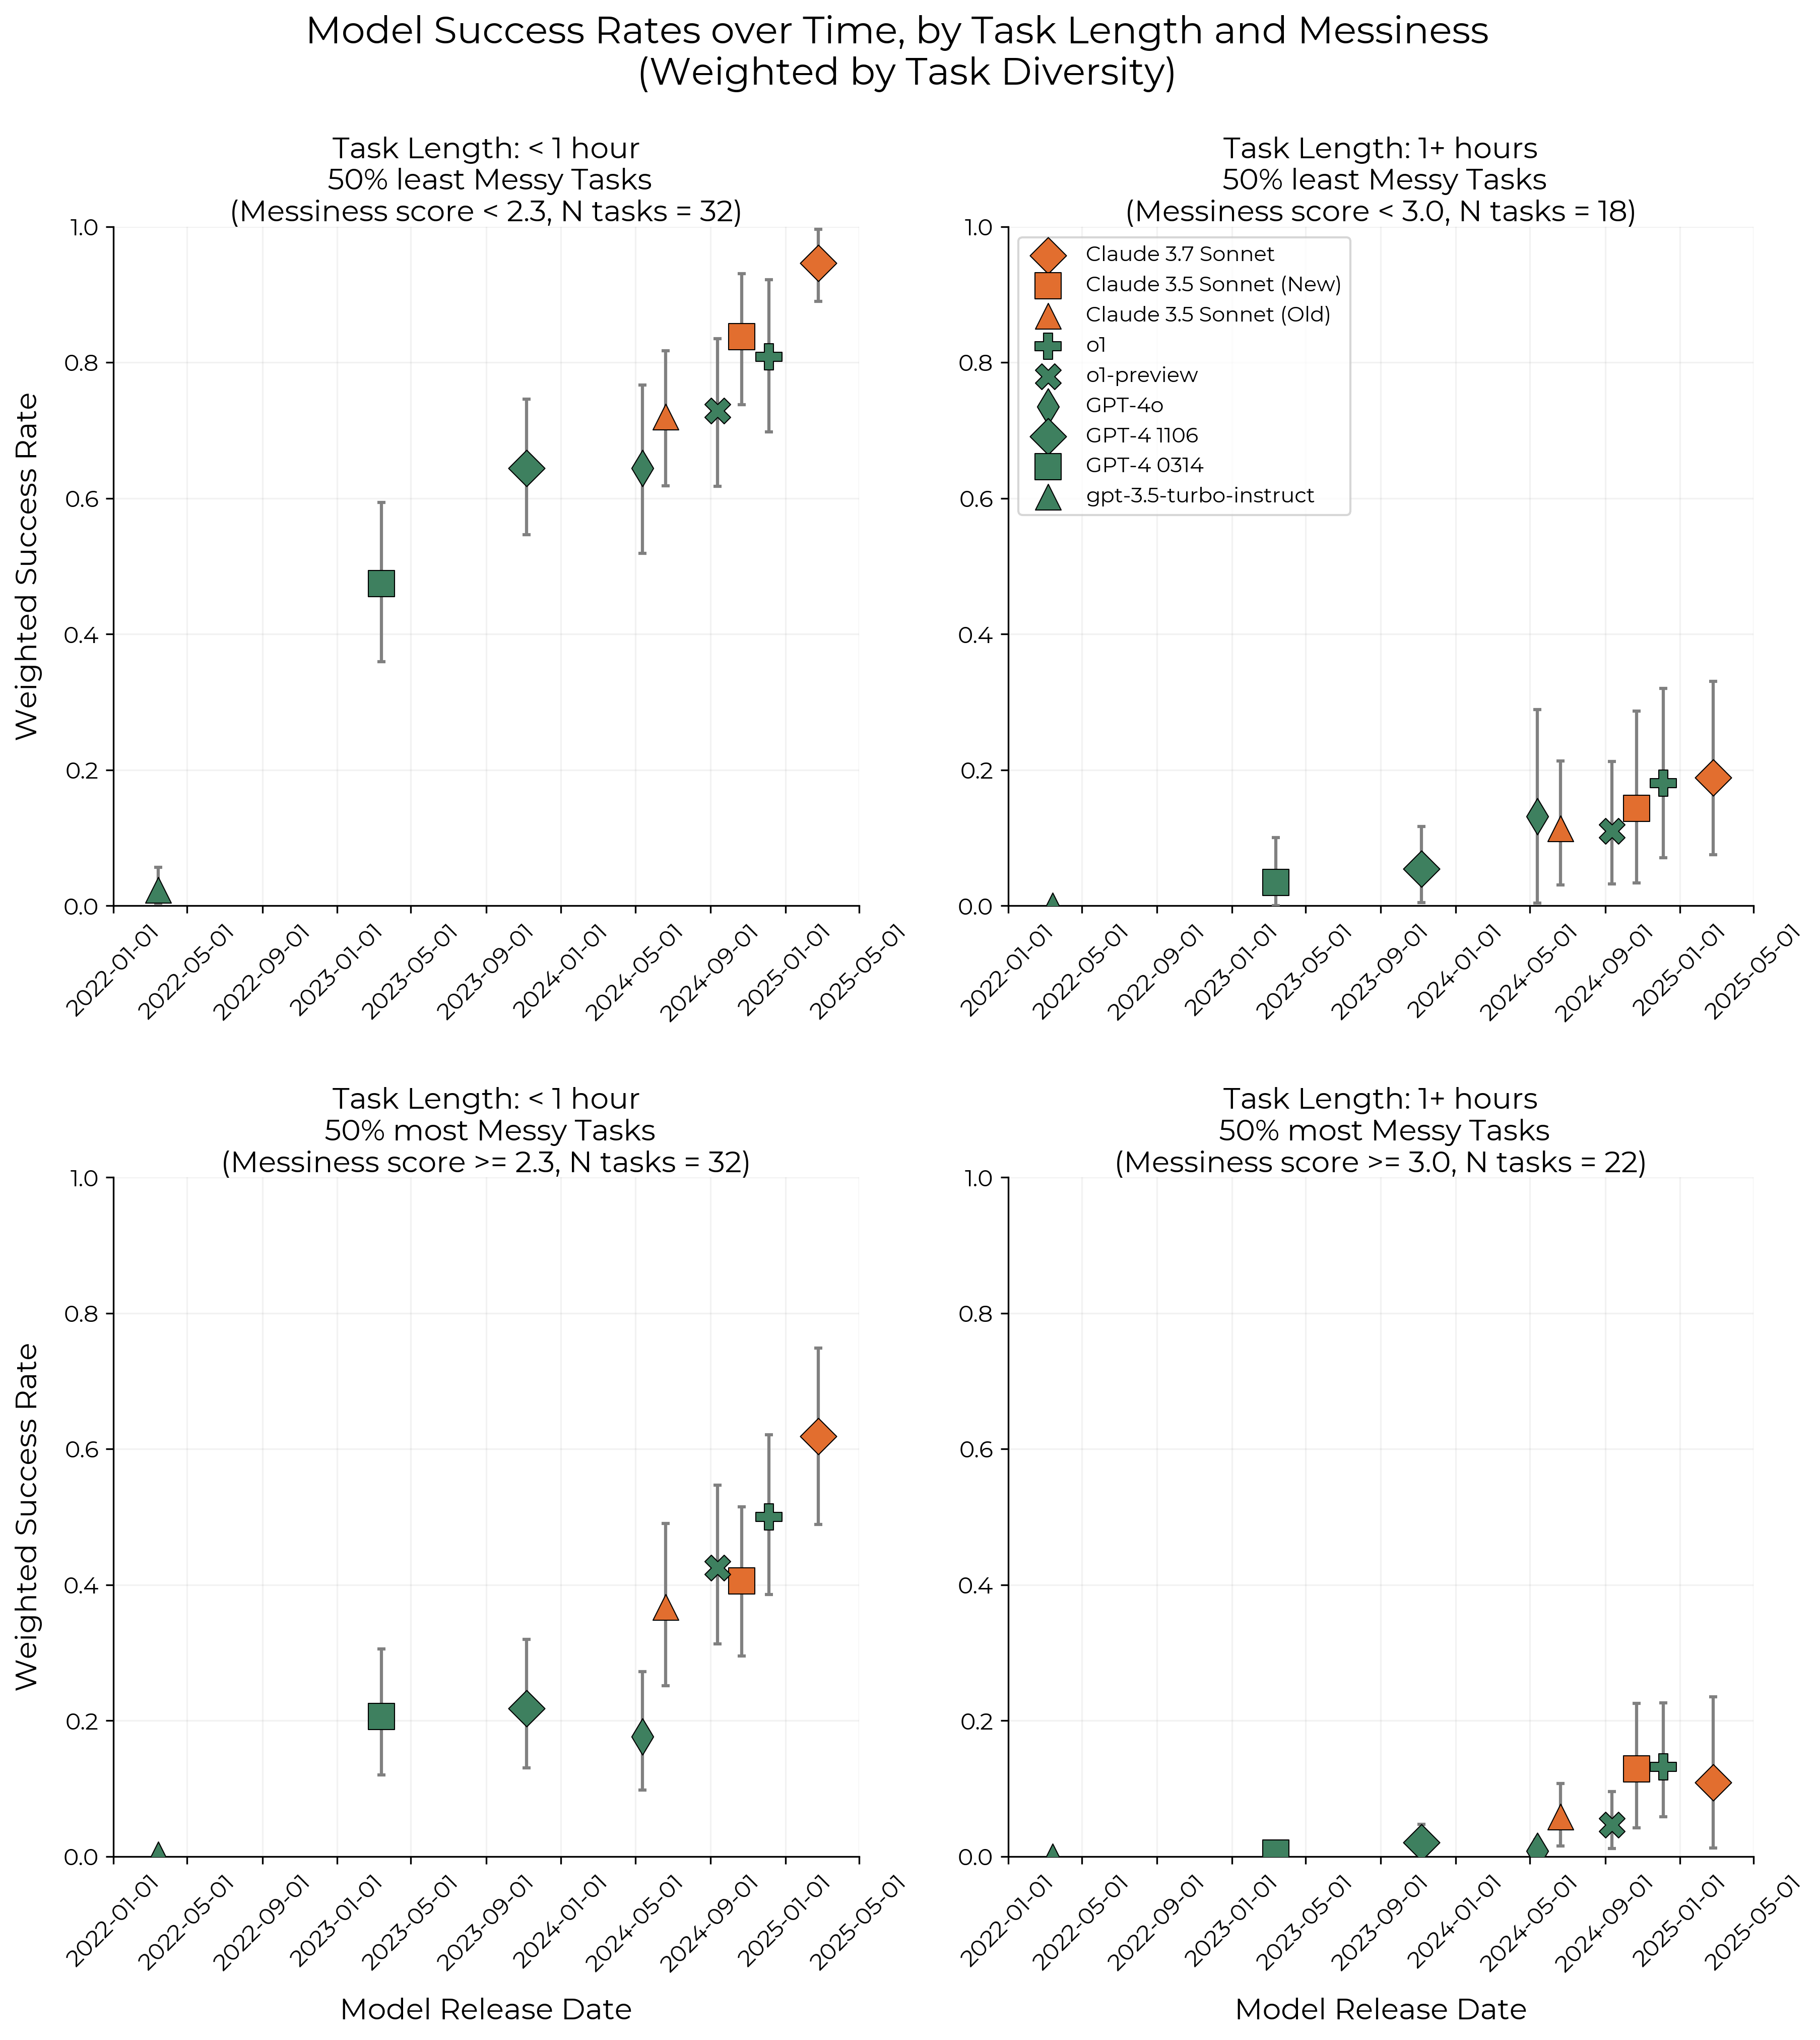
\includegraphics[width=0.9\linewidth]{plots/messiness/success_trend_by_messiness_and_length_with_boundary_0.5.png}
    \caption{Performance trends over time for \gabenchmark{} and RE-Bench tasks by length and messiness (Section~\ref{sec:messiness-split}). The data spans only 2023--2024 as pre-2023 models score 0 on non-SWAA tasks. Whilst our messier tasks have lower average success rates, trends in model performance improvements are not obviously slower on the high messiness split.}
    \label{fig:2x2}
\end{figure}

We rated \gabenchmark{} and RE-Bench tasks on 16 properties that we expected to be 1) \textbf{representative} of how real world tasks might be systematically harder than our tasks and 2) \textbf{relevant} to AI agent performance. Some example factors include whether the task involved a novel situation, was constrained by a finite resource, involved real-time coordination, or was sourced from a real-world context. We labeled RE-bench and \gabenchmark{} tasks on the presence or absence of these 16 messiness factors, then summed these to obtain a ``messiness score'' ranging from 0 to 16. Factor definitions can be found in Appendix~\ref{app:messiness}.

The mean messiness score amongst \gabenchmark{} and RE-Bench tasks is 3.2/16. None of these tasks have a messiness score above 8/16. For comparison, a task like 'write a good research paper' would score between 9/16 and 15/16, depending on the specifics of the task.

On \gabenchmark{} tasks, AI agents do perform worse on messier tasks than would be predicted from the task's length alone (b=-0.081, $R^2$ = 0.251), see Figure~\ref{fig:observed-predicted-messiness}. An increase in task messiness by 1 point reduces mean success rates by roughly 8.1\%\footnote{A linear approximation of this relationship is used for the purpose of roughly quantifying the size of this effect in an intuitive way.}.

However, trends in AI agent performance over time are similar for lower and higher messiness subsets of our tasks. For example, on sub hour tasks, success rates increased by 40 percentage points between Jan. 2023 and May 2025 in both high and low messiness splits (Figure~\ref{fig:2x2}). In particular, we find no evidence of either much slower performance trends, or a plateau, specific to our higher messiness subset. 

\begin{figure}
    \centering
    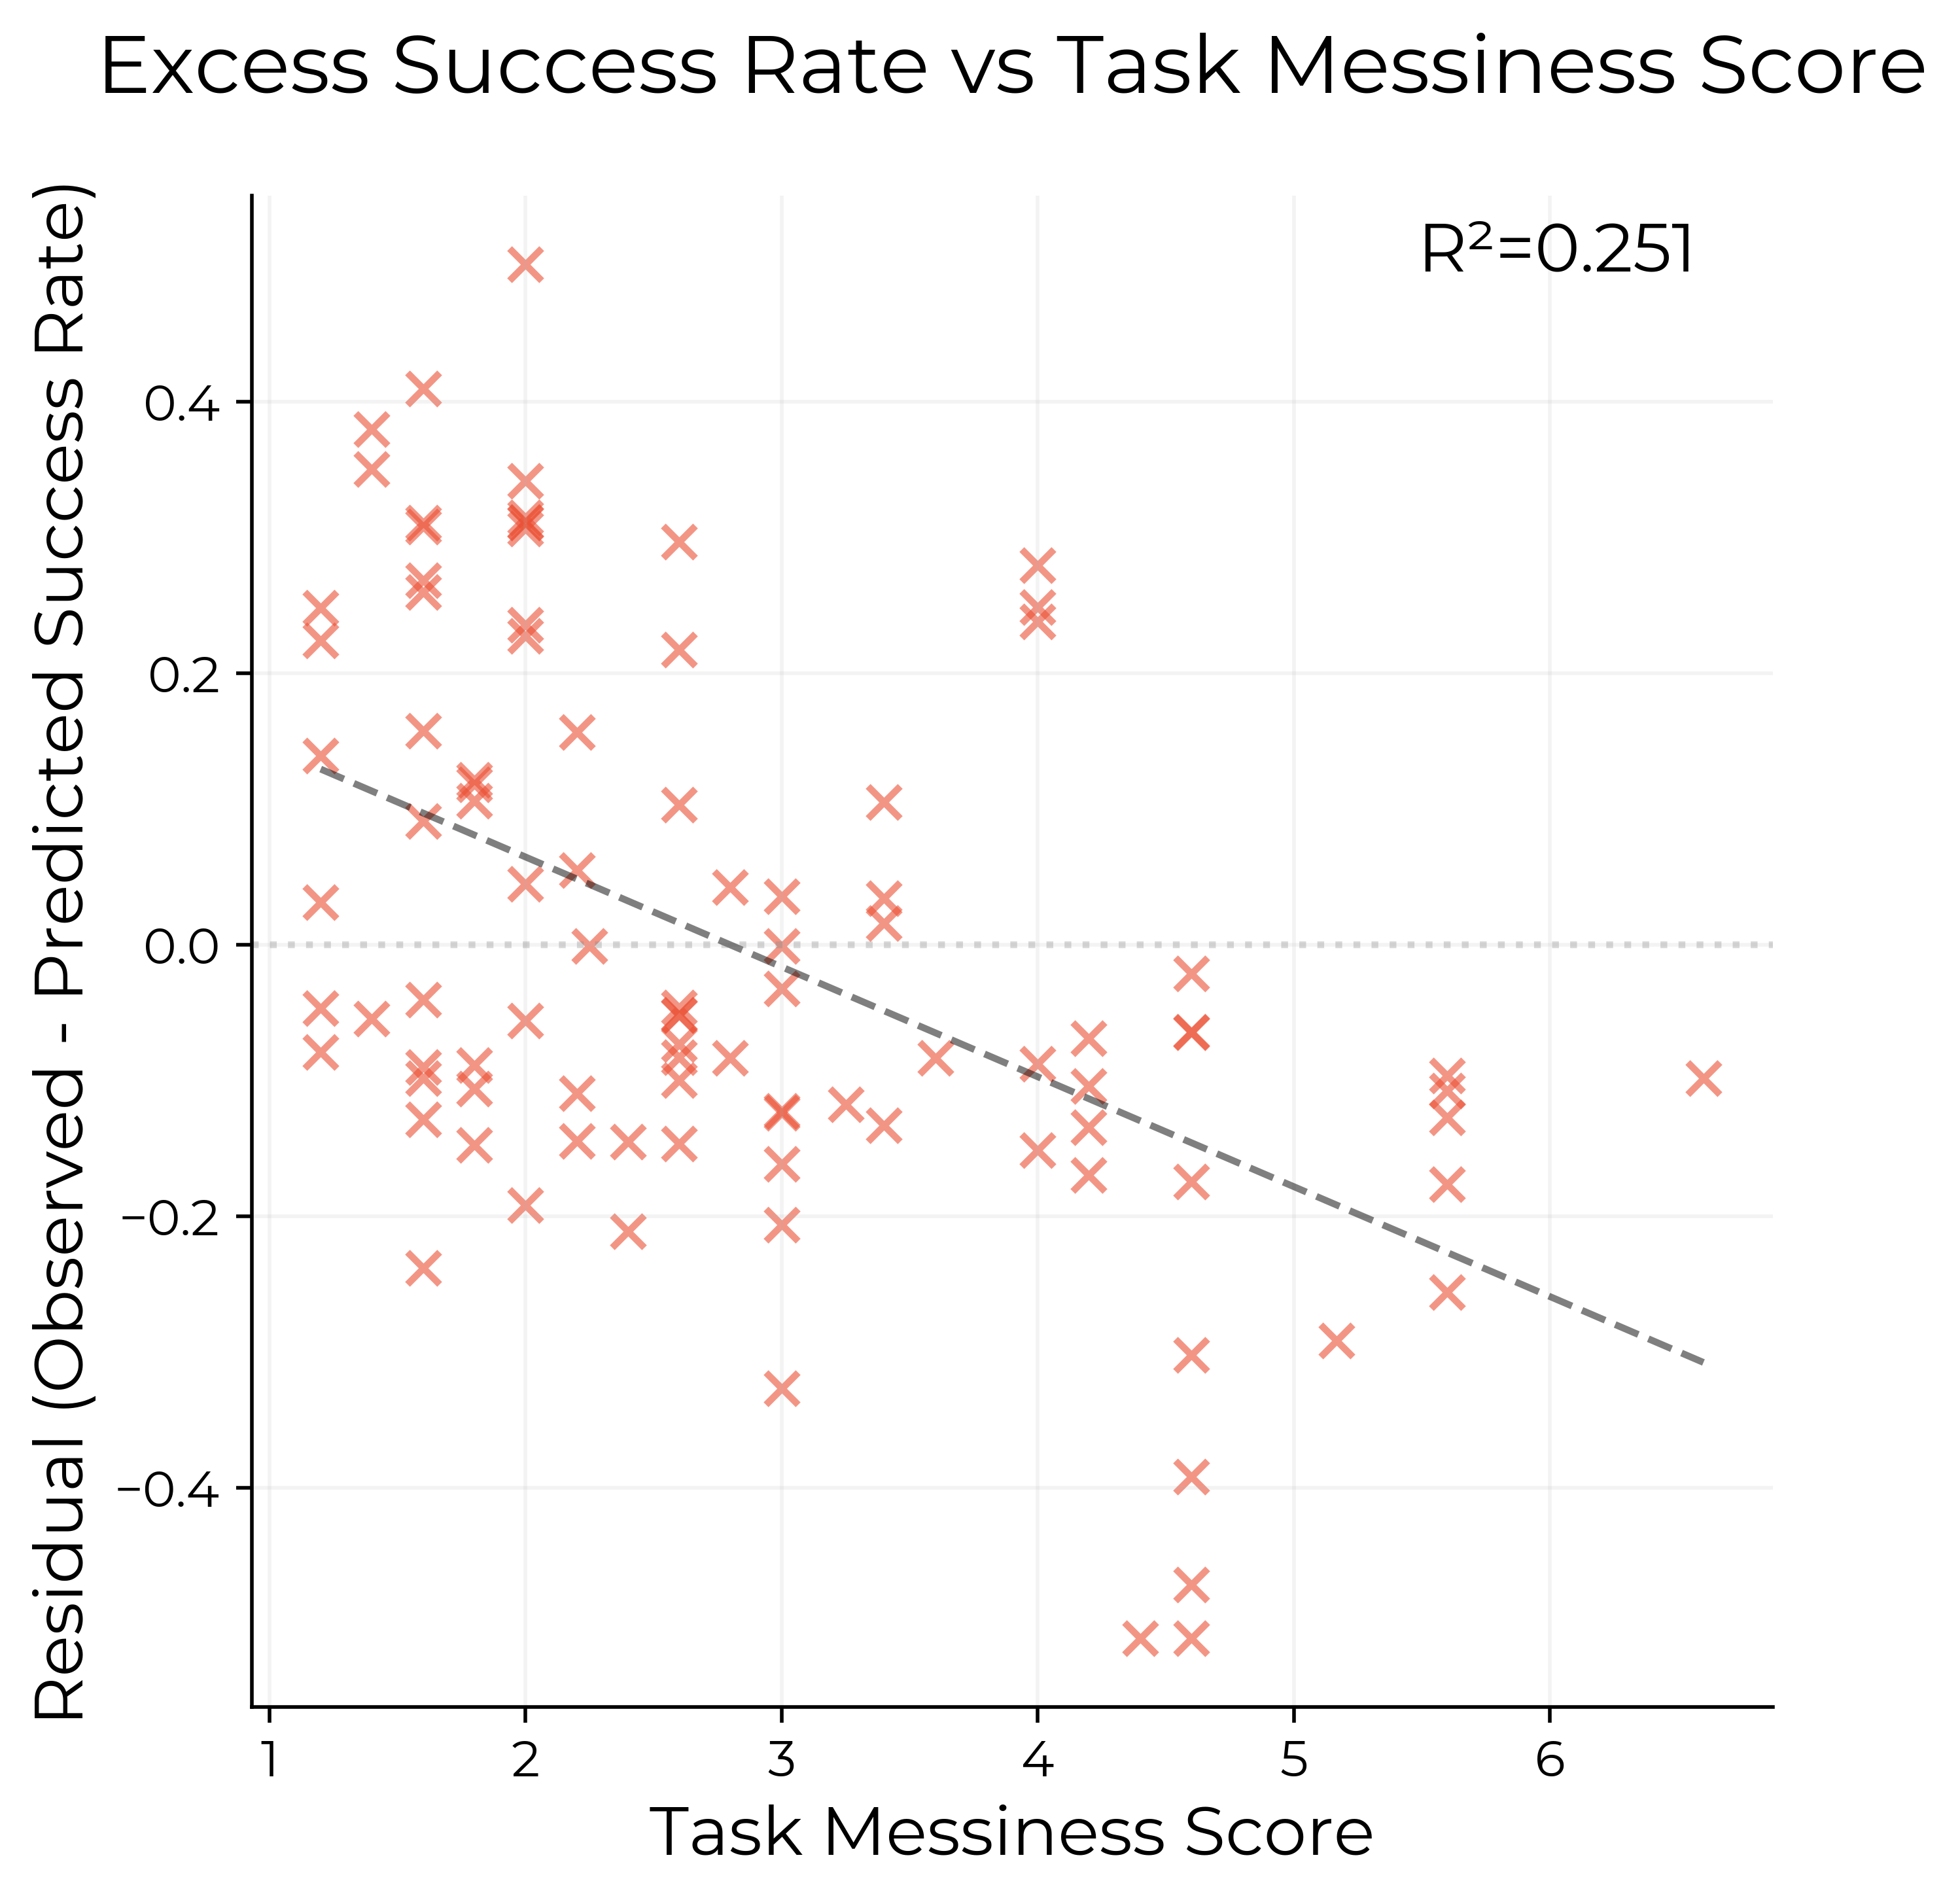
\includegraphics[width=0.5\linewidth]{plots/messiness/messiness_effect_expanded_combined_alpha_0.010.png}
    \caption{We plot the excess success rate (the observed empirical task success rate, minus success rate we would predict using the task's length, see Section~\ref{sec:model_horizon_length}) against messiness score for each task. As discussed in Section~\ref{sec:messiness-split}, there is a negative relationship between excess success rates and messiness.}
    \label{fig:observed-predicted-messiness}
\end{figure}

\subsection{SWE-bench Verified} \label{sec:swebench}

To check whether we observe similar performance trends in time horizon on other benchmarks, we apply our methodology to SWE-bench Verified. SWE-bench Verified is an industry standard benchmark for evaluating language model performance on software engineering tasks \cite{o3mini}. All tasks in the SWE-bench Verified dataset were harvested from large open source repositories, like matplotlib or django, and then filtered to ensure they are automatically checkable and well-specified \cite{jimenez2024swebench}.

\begin{figure}
    \centering
    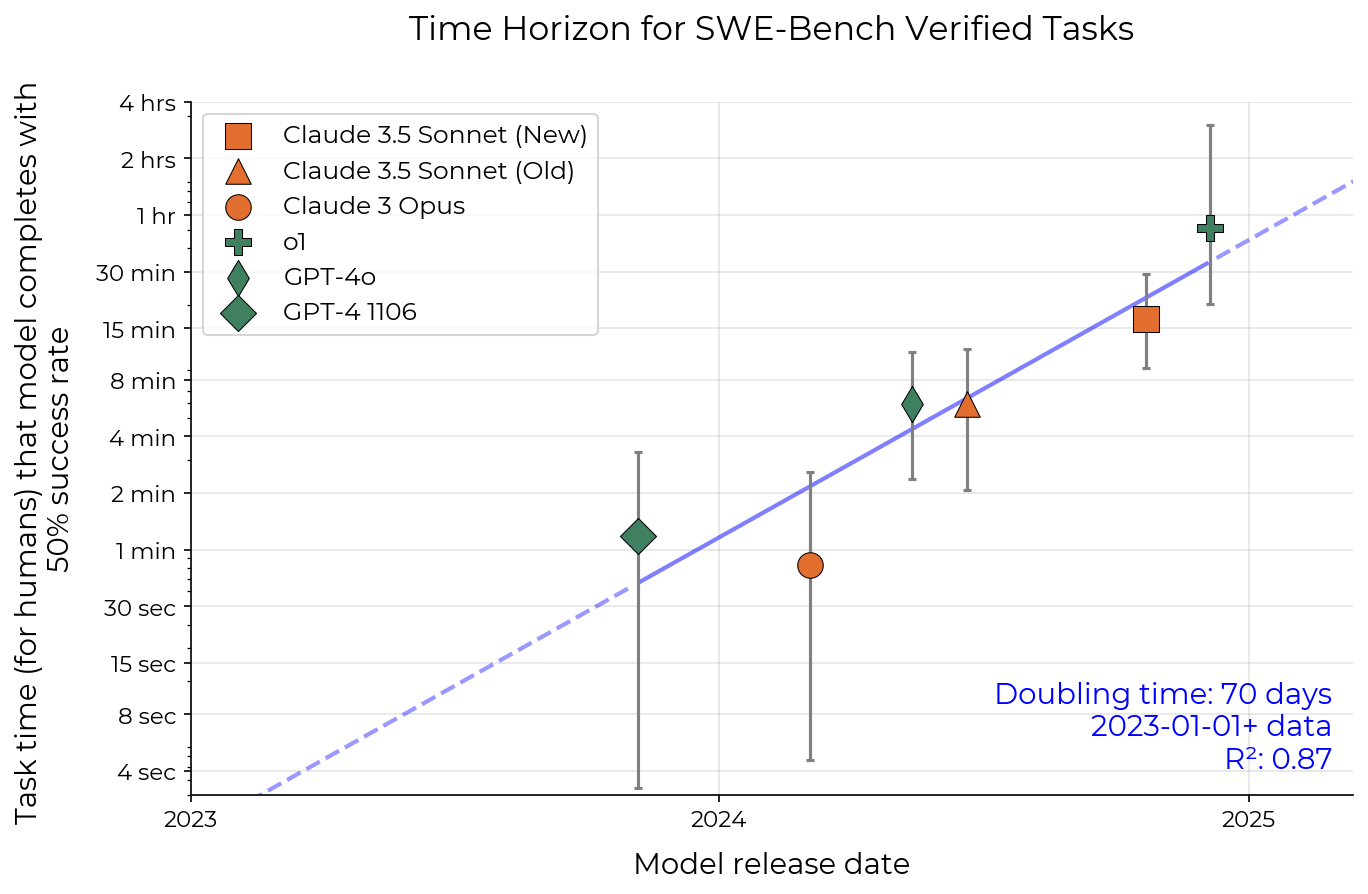
\includegraphics[width=0.8\linewidth]{plots/logistic/swe_bench.png}
    \caption{Performance of frontier AI models using reported SWE-bench Verified results (Section~\ref{sec:swebench}). We observe a similar exponential trend to Figure~\ref{fig:headline}, albeit with a steeper slope.}
    \label{fig:swebench}
\end{figure}

Model time horizon computed from SWE-bench Verified tasks seem to follow an exponential trend from late 2023 through 2024. However, while the doubling time predicted by \gabenchmark{} + SWAA + RE-bench using 2024 models is 104 days, the doubling time predicted by the SWE-bench Verified results is shorter---around 70 days. 

SWE-bench Verified time annotations were based on the expected time it would take an ``engineer who has had a few hours to familiarize themselves with the codebase" to solve the issue \cite{jimenez2024swebench}. We found that annotator time estimates differentially underestimate how long our contract baseliners take to complete the easiest SWE-bench verified tasks. As a result, our time horizon estimates for SWE-bench Verified (which use annotator times) are likely to underestimate the time horizon of less capable models relative to contractor times, in turn shortening doubling times. For more details see Appendix \ref{app:swe-bench}. 


\subsection{Internal PR experiments}\label{internal-prs}
We also  ran GPT-4o, Claude 3.5 Sonnet (New), and o1 on five uncontaminated issues from an internal METR repository. Resolving these issues was real work performed by METR staff, so we might expect results on these tasks to better represent performance on real economically valuable tasks than a typical benchmark task.

We find that our contract baseliners take 5x-18x longer to resolve issues than repository maintainers. Additionally, AI agent performance on these issues is not inconsistent with AI agent success rate curves derived from \gabenchmark{}, SWAA, and RE-Bench performance if \textit{contractor} time-to-complete is used to measure the tasks length. However, it takes much longer for our contract baseliners to complete these tasks than repository maintainers. This suggests that time horizons may have better correspondence to the labor of a low-context human, rather than a high-context human. See Appendix \ref{internalprtasksdetails} for methodological details and more results.

\section{Extrapolation} \label{sec:extrapolation}

\subsection{Extrapolating towards one-month-horizon AI} \label{trend_sensitivity} 

When forecasting when AI systems will be capable of autonomously generating large economic value and when they will be capable of catastrophic actions, it is necessary to choose a concrete threshold for horizon length. We chose one month (approximately 167 working hours for a fair comparison with humans, since humans cannot work 24/7) for two reasons. First, \citet{ngo2023tagi} writes that a 1-month AGI (defined as an AI that outperforms most knowledgeable humans who are given 1 month of work hours, i.e. 167 hours, to perform the task) would necessarily exceed human performance both at tasks including writing large software applications or founding startups (clearly economically valuable), and including novel scientific discoveries.\footnote{Note that our forecasts concern AI with a 1-month horizon on software tasks, not 1-month AGI, because we evaluate models only on software and research tasks. Nevertheless, given past correlations in different areas of AI performance, 1-month (167 hours) time horizon AI may be significantly generally capable.} Second, one month is around the period when new hires at a company begin to complete onboarding and generate economic value,\footnote{Onboarding ``can last from a few weeks to more than a year'' \citep{zielinski_optimize_onboarding}, and employees often start generating economic value midway through the onboarding process.} and so an AI with a horizon of 1 month could be capable of acquiring context like a human employee, allowing it to complete high-context as well as low-context tasks.

In this section, we attempt to forecast when AIs will reach a 50\%-time horizon of 1 month, because it intuitively seems that a system capable of this length of task, even at 50\% reliability, would be transformative for our society, including potentially being proficient in capabilities that could threaten society with catastrophic harm.

\begin{figure}
    \centering
    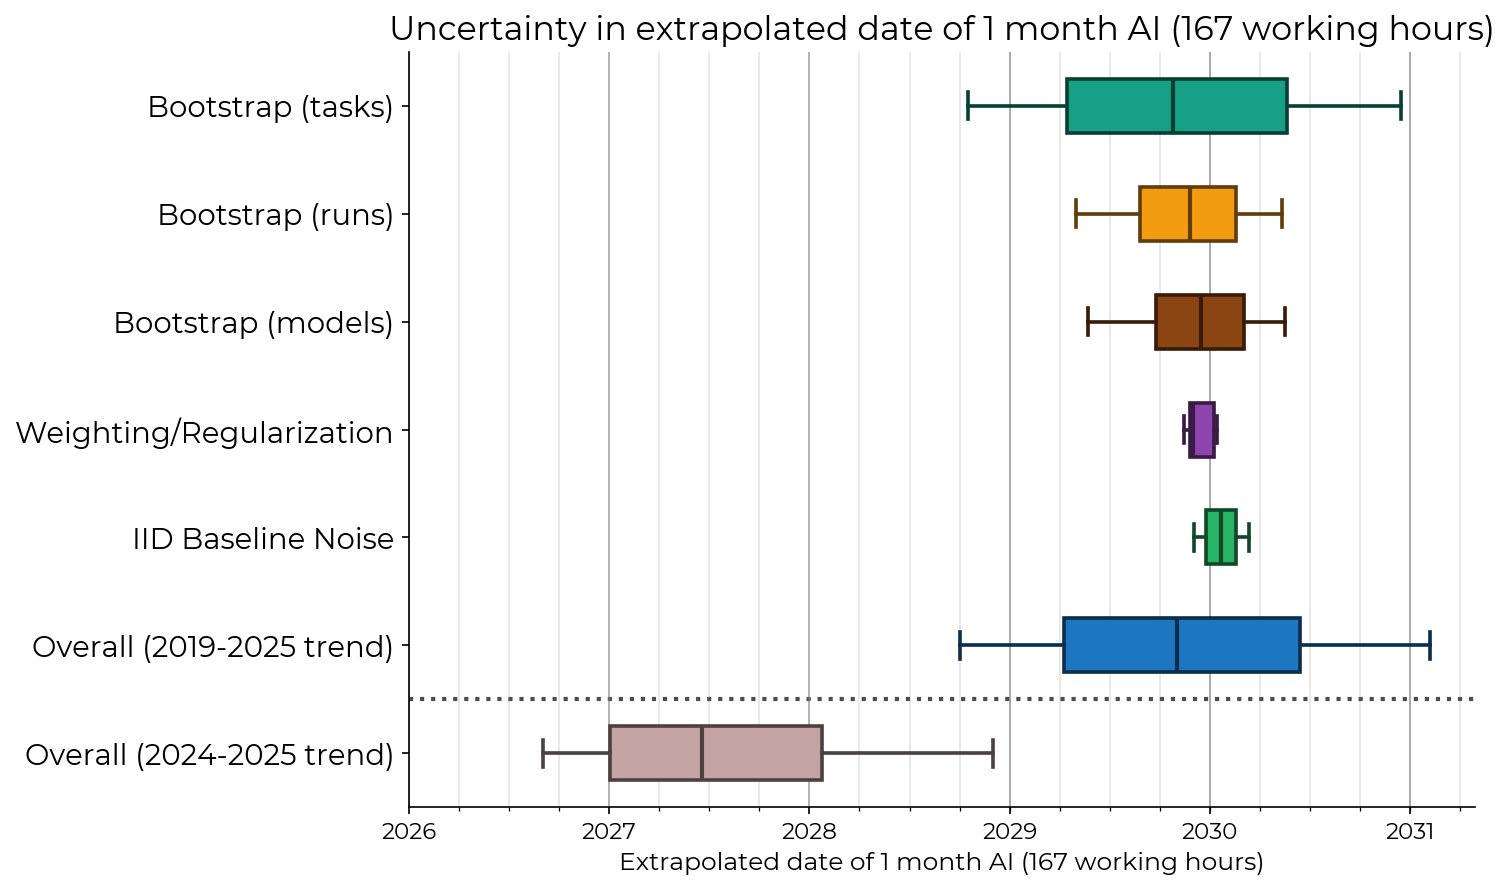
\includegraphics[width=0.8\linewidth]{plots/multiverse/boxplot.png}
    \caption{A sensitivity analysis of the extrapolated date at which frontier AI systems will have a horizon of 1 month. In each row, we apply 10,000 random perturbations to our data and find the distribution over the date of 1-month AI implied by the perturbed data.
    Box endpoints represent the 25th and 75th percentiles, and whiskers the 10th and 90th percentiles, with outliers not displayed. Note that this plot does not account for future changes in the trend or external validity concerns, which are responsible for the majority of our uncertainty.}
    \label{fig:multiverse-boxplot}
\end{figure}

\paragraph{Sensitivity analysis} Although extrapolation is always imperfect, forecasting AI horizon lengths far into the future is much more sensitive to changes in doubling rate than to constant factors in horizon length. For example, a naive extrapolation based on o1's time horizon of 39 minutes and a past doubling time of 218 days (3.2x/year) predicts that AIs will reach a 1-month 50\% time horizon (roughly 8 doublings over o1) about 4.8 years after the release date of o1. A 2x increase in doubling time would delay the 1 month point by a further 4.8 years, but a 2x constant factor decrease in horizon length would only delay it by 0.6 years.

Figure~\ref{fig:multiverse-boxplot} shows a sensitivity analysis of our results over various sources of noise. ``Bootstrap (tasks)" reflects our limited number of tasks and the fact that tasks of the same human duration vary in difficulty for models, while ``Bootstap (runs)'' derives from our limited number of runs; the combination of these two is shown as the confidence region in Figure~\ref{fig:headline}. ``Bootstrap (models)" represents the limited number of models in our dataset. ``Weighting/regularization" represents methodological choices; this perturbation includes 10 hyperparameter combinations with and without task diversity weighting, and with a logistic regression regularization parameter between 0.01 and 0.2. ``IID Baseline Noise'' multiplies every task duration by a random factor based on the empirical distribution of baseline times. We combine these into an overall estimate of uncertainty in the past trend, and do the same for the 2024--2025 only trend (note that our confidence in this trend is much lower because there are only six models in this time span).

Because our analysis puts low probability on the growth rate of time horizon on our tasks being much slower than one doubling every 8 months, the uncertainty in the extrapolated date of 1-month AI is fairly small (80\% CI width about 2 years, central estimate late 2029). Bootstrapping over our task distribution and runs contributes most of the uncertainty, representing our limited task dataset and the variance in difficulty (for models) between tasks of the same human length, as well as run-to-run variance. If future progress instead follows the 2024--2025 trend, 1-month AI would arrive sooner, with half the probability in 2027 and early 2028. 

It is possible that systematic biases and alternate methodologies have a greater impact on forecasts, and we discuss these in Appendix~\ref{app:robustness}. In addition, due to the inherent difficulty of predicting the future, real forecasts will have larger error than this naive extrapolation, which we discuss below.

\subsection{Difficulties in extrapolation} \label{sec:predicting-future-trends}

Most of our uncertainty about the future comes from (a) applicability to real tasks, partly discussed in Section~\ref{sec:externalvalidity}, and (b) future changes in the time horizon growth rate. 

\subsubsection{Systematic differences between our tasks and real tasks}

The tasks we use to benchmark AI capabilities are systematically different from real tasks. These differences could result in the trends we observe on our tasks not generalizing to real world tasks. For instance, all SWAA, \gabenchmark{}, and RE-Bench differ from real-world tasks in the following ways:
\begin{itemize}
    \item \textbf{Automatic scoring} All tasks we use are automatically scorable, meaning a piece of code running in the task environment determines the final score. This imposes constraints on e.g. the format of solutions, that tend to reduce task open-endedness, and the need for sensible value judgments. 
    \item \textbf{No interaction with other agents} None of our tasks involve interacting with other autonomous agents. Coordinating with, or competing with, other agents seems likely to increase task difficulty. For instance, by increasing the importance of strategic decision-making, real-time coordination, and predicting the actions of other complex agents.
    \item \textbf{Lax resource constraints} None of our SWAA tasks, and few of our \gabenchmark{} tasks saliently involve making efficient use of a limited resource---a common constraint in real-world tasks.
    \item \textbf{Unpunishing} Similarly, very few of our tasks are punishing of single mistakes.\footnote{With the exception of submitting an answer too early on \gabenchmark{} tasks.} This is in part to reduce the expected cost of collecting human baselines. Real world tasks can often be more punishing, for instance, when they involve competing against other agents. For instance, a single blunder in a chess game can greatly reduce the chance of winning the game. 
    \item \textbf{Static environments} Our tasks typically use environments that do not significantly change unless directly acted upon by the agent. In contrast, real tasks often occur in the context of a changing environment.
\end{itemize}

We attempted to measure how these systematic differences might affect AI agent performance in Section \ref{sec:messiness-split}, by including the above properties as ``messiness" factors. We found that though the absolute performance on ``messier" tasks was lower, the trends in performance were similar to less messy tasks. Even so, these systematic differences cast doubt on whether the rapid performance improvements seen on our tasks (and other benchmarks like SWE-Bench Verified) will generalize to real world tasks. 

Regardless of whether or not this trend generalizes to real world tasks, we believe our results to be significant. If our results do not generalize to real tasks, then benchmarks like \gabenchmark{} and SWE-Bench Verified may be insufficient for forecasting AI capabilities on real tasks, and we may need more realistic benchmarks. On the other hand, if our results do generalize to real tasks, then extrapolating our trend predicts that AIs capable of automating a month of human software development will be made before 2032.

\subsubsection{Future changes in time horizon trends}

Here, we discuss three additional possible factors that could significantly change the time horizon growth rate: agency training, compute scaling, and automation of AI research and development. 

\paragraph{Agency training} Horizon growth since 2024, which may be faster than the long-term trend, could be explained by researchers post-training models to be more agentic (that is, capable of taking many sequential actions towards completing a task) using outcome-based RL. Research into making models capable and agentic is likely to continue. Future agency training could be faster than the long-run trend (since post-training may be more compute-efficient than pretraining at increasing horizon length). But 2024--2025 agency training could also be a one-time boost from picking low-hanging fruit, in which case horizon growth will slow once these gains are exhausted. Overall, we think agency training is more likely to increase the time horizon growth rate compared to the 2019--2024 trend.

\paragraph{Compute scaling} Between the release of GPT-2 and today, the compute used to train the most impressive frontier language models has increased by at least a factor of 10,000x \cite{EpochNotableModels2024}, with training compute usage doubling every 6--10 months \cite{sevilla2022compute}. More recently, models like o1 and o3 have began to use more compute at inference time. It is unclear whether there is sufficient capacity to expand either training or inference compute by many more orders of magnitude in the next 5 years. However, algorithmic improvements, which have historically decreased the compute requirements for a fixed performance level \citep{erdil2023algorithmicprogresscomputervision} \citep{ho2024algorithmicprogresslanguagemodels}, can substitute for compute limitations. We think that limits to compute scaling will slow the growth of AI agent time horizons somewhat, but be partially compensated by more investment into algorithmic improvement.

\paragraph{Automation of AI R\&D} The main inputs to AI research and development are compute and researcher time. If future AI systems are capable of substituting for human research engineers and/or increasing the compute-efficiency of training, the rate of AI progress will increase. We think it is likely that there will be substantial AI R\&D automation once frontier AI time horizon reaches tens of hours, shortening the time from then until one-month-horizon AI.

\section{Discussion} \label{sec:discussion}


\subsection{Measuring and interpreting time horizon} \label{sec:interpretation_horizon}

Although time horizon is an intuitive measure of AI agent capability, measuring it requires a large dataset annotated with human time, and time horizon is always measured relative to a task distribution and baseliners' levels of context and skill.

\paragraph{Context and skill effects}

At real companies, junior software engineer hires often take weeks of onboarding to begin contributing economic value. The human baseliners that determine the length of our tasks have much less context than average employees, potentially \textit{increasing} measured task length. Our tasks are designed to require minimal context, which somewhat mitigates this problem; our internal PRs (Section \ref{internal-prs}) were not designed this way, and so baseliners took many times longer than employees. However, highly skilled baseliners can also complete tasks far faster than average employees. Our expert baseliners are likely much more skilled than the average software engineer, potentially \textit{decreasing} our measured task length.

\paragraph{Task distribution effects} Figure~\ref{fig:success_vs_time} shows that AI agent success rate is imperfectly predicted by human time-to-complete, meaning that other factors also substantially influence the difficulty of tasks. When models are measured in different domains of intellectual labor like research mathematics, computational biology, or law, we expect their time horizons to differ.

\paragraph{Measuring extreme time horizons} \label{sec:measuring-extreme-time-horizons} Accurately measuring that the X\%--time horizon of an AI agent is about $t$ minutes requires many tasks of human length $t$ that the AI agent completes with a success rate of about X\%. This has two implications. First, accurately measuring very long time horizons requires a dataset of difficult tasks with long human baseline runs, which can be impractical to construct, especially because success criteria for realistic difficult tasks are often complex enough to require manual grading. Second, measuring time horizons at extremely high success levels-- 95\%, 98\%, or higher-- requires very large task datasets with near-zero label noise that cover the population of tasks they are meant to represent.

\paragraph{AGI will have ``infinite" horizon length} An infinite time horizon does not mean an arbitrarily capable AI, merely the ability to complete tasks that take humans an arbitrarily long length of time. If an artificial general intelligence (AGI) is capable of completing \textit{all} tasks expert humans can with a success rate of at least X\%, its X\% time horizon will necessarily be infinite. Therefore, if such systems are ever developed, the long-term trend in time horizon will be faster than exponential, with an asymptote at the date of AGI deployment.

\paragraph{Human time horizon measurements} In theory, one could also measure the time horizon of a human or population of humans. However, there are both theoretical and practical difficulties to doing so. We discuss this more in Appendix~\ref{app:baseline-success-rate}.

\subsection{Limitations and future work}
We believe that there are several ways in which our work could be improved.

\paragraph{More models with better elicitation}\label{sec:more_elicitation}
In general, we find that properly eliciting models can make a very large difference in their performance.\footnote{This is a common obervation; see e.g. the improvements to software development capabilities from AIDE \cite{jiang2025aide}
or METR's recent work on KernelBench: \url{https://metr.org/blog/2025-02-14-measuring-automated-kernel-engineering/}.}
We have put a limited amount of effort into eliciting models to get good performance on our tasks, so while our results are a reasonable lower bound, some models may have somewhat greater capabilities than we demonstrate. 
The most work was done to elicit o1 and the original Claude 3.5 Sonnet, each of which had around 2-3 engineer weeks of iterative development. All other models use the same scaffolding with at most minor changes. 
Future work could replicate our results with more effort spent on eliciting the full capabilities of frontier models. 

\paragraph{More rigorous human baselining}
Our per-task human time estimates are likely noisy due to relatively small sample size, and potentially also systematically skewed in various ways. 
Most notably, we select only successful completions of a task, and encourage baseliners to give up on tasks they may not complete in a reasonable amount of time. 
Our baseliners' skills also vary significantly, and a wide variety of skills are relevant to our tasks. 
Though we attempt to match baseliners with appropriate tasks, this process is unlikely to be perfect. 
From manual reviews of baseline attempts, we also observe that humans sometimes simply give up even when the task seems within their capabilities, and it is unclear what selection effects are produced on the distribution of success times as a result.
% Overall, we have significant uncertainty about baseline times, but these times will not significantly affect the long-run trend (\ref{trend_sensitivity}) unless there is a systematic bias correlated with task length (as may be true in SWE-bench Verified \ref{sec:swebench}) or a large constant factor.
See See Appendix~\ref{app:baseline-success-rate} for further discussion of how bias in human baseline times could affect our results. Future work could replicate our results with more rigorous human baseliner selection or explore how sensitive the results are to methodological choices around human baselining. 

\paragraph{More natural, varied tasks}
There are reasons to believe that our task distribution is systematically different from the distribution of economically valuable work (and perhaps systematically different than the distribution of risk-model relevant tasks). 
We explored some of these reasons in Sections~\ref{sec:externalvalidity}, but there remain many differences that we did not explore.
For example, the modality of interaction in our tasks is also relatively narrow---for example, none of our tasks require the use of a mouse. 
None of our tasks require cooperating or competing with humans or other agents,\footnote{See \citet{xu2024theagentcompany} for an example of a recent benchmark that requires multi-agent interaction in a relatively realistic setting.} while real software engineering or ML research involves communicating and coordinating with managers and other engineers or researchers. Many real-world tasks require very high reliability, and these are underrepresented in our dataset due to the difficulty of measuring models on these tasks.
Most importantly, the tasks we study are heavily skewed toward software engineering and ML research. 
Future work could explore how the capabilities of AI agents are progressing in other domains. 

\paragraph{More use of inference compute} Our scaffolds made relatively limited use of inference-time compute. When assuming that the human expert is compensated at \$143.61/hour (average L4 Engineer salary at Google divided by 2,000 hours), more than 80\% of successful runs cost less than 10\% of what it would cost for a human to perform the same task. (Figure \ref{fig:cost-ratio}). This implies that if inference-time computation could be used to improve performance, there is substantial room to do so while still remaining economically competitive with human experts. Previous research has found that techniques such as best-of-k can substantially improve performance on a subset of these tasks,\cite{wijk2024re} and better use of inference-time compute may lead to substantially different scores. 

\paragraph{Data analysis} The 2024--2025 trend appears faster than the 2019--2025 trend, but due to the small number of models it is unclear if this is noise. Future work should include hypothesis testing to detect a possible 2024 slope change, and more sophisticated statistical methods to create credible intervals for an overall forecast. We also lose some information in the multiple stages of estimation---conversion of baseline data to task difficulty ratings, time horizon computation, and linear regression to find the trend---and end-to-end methods could be more data-efficient.

\begin{figure}
    \centering
    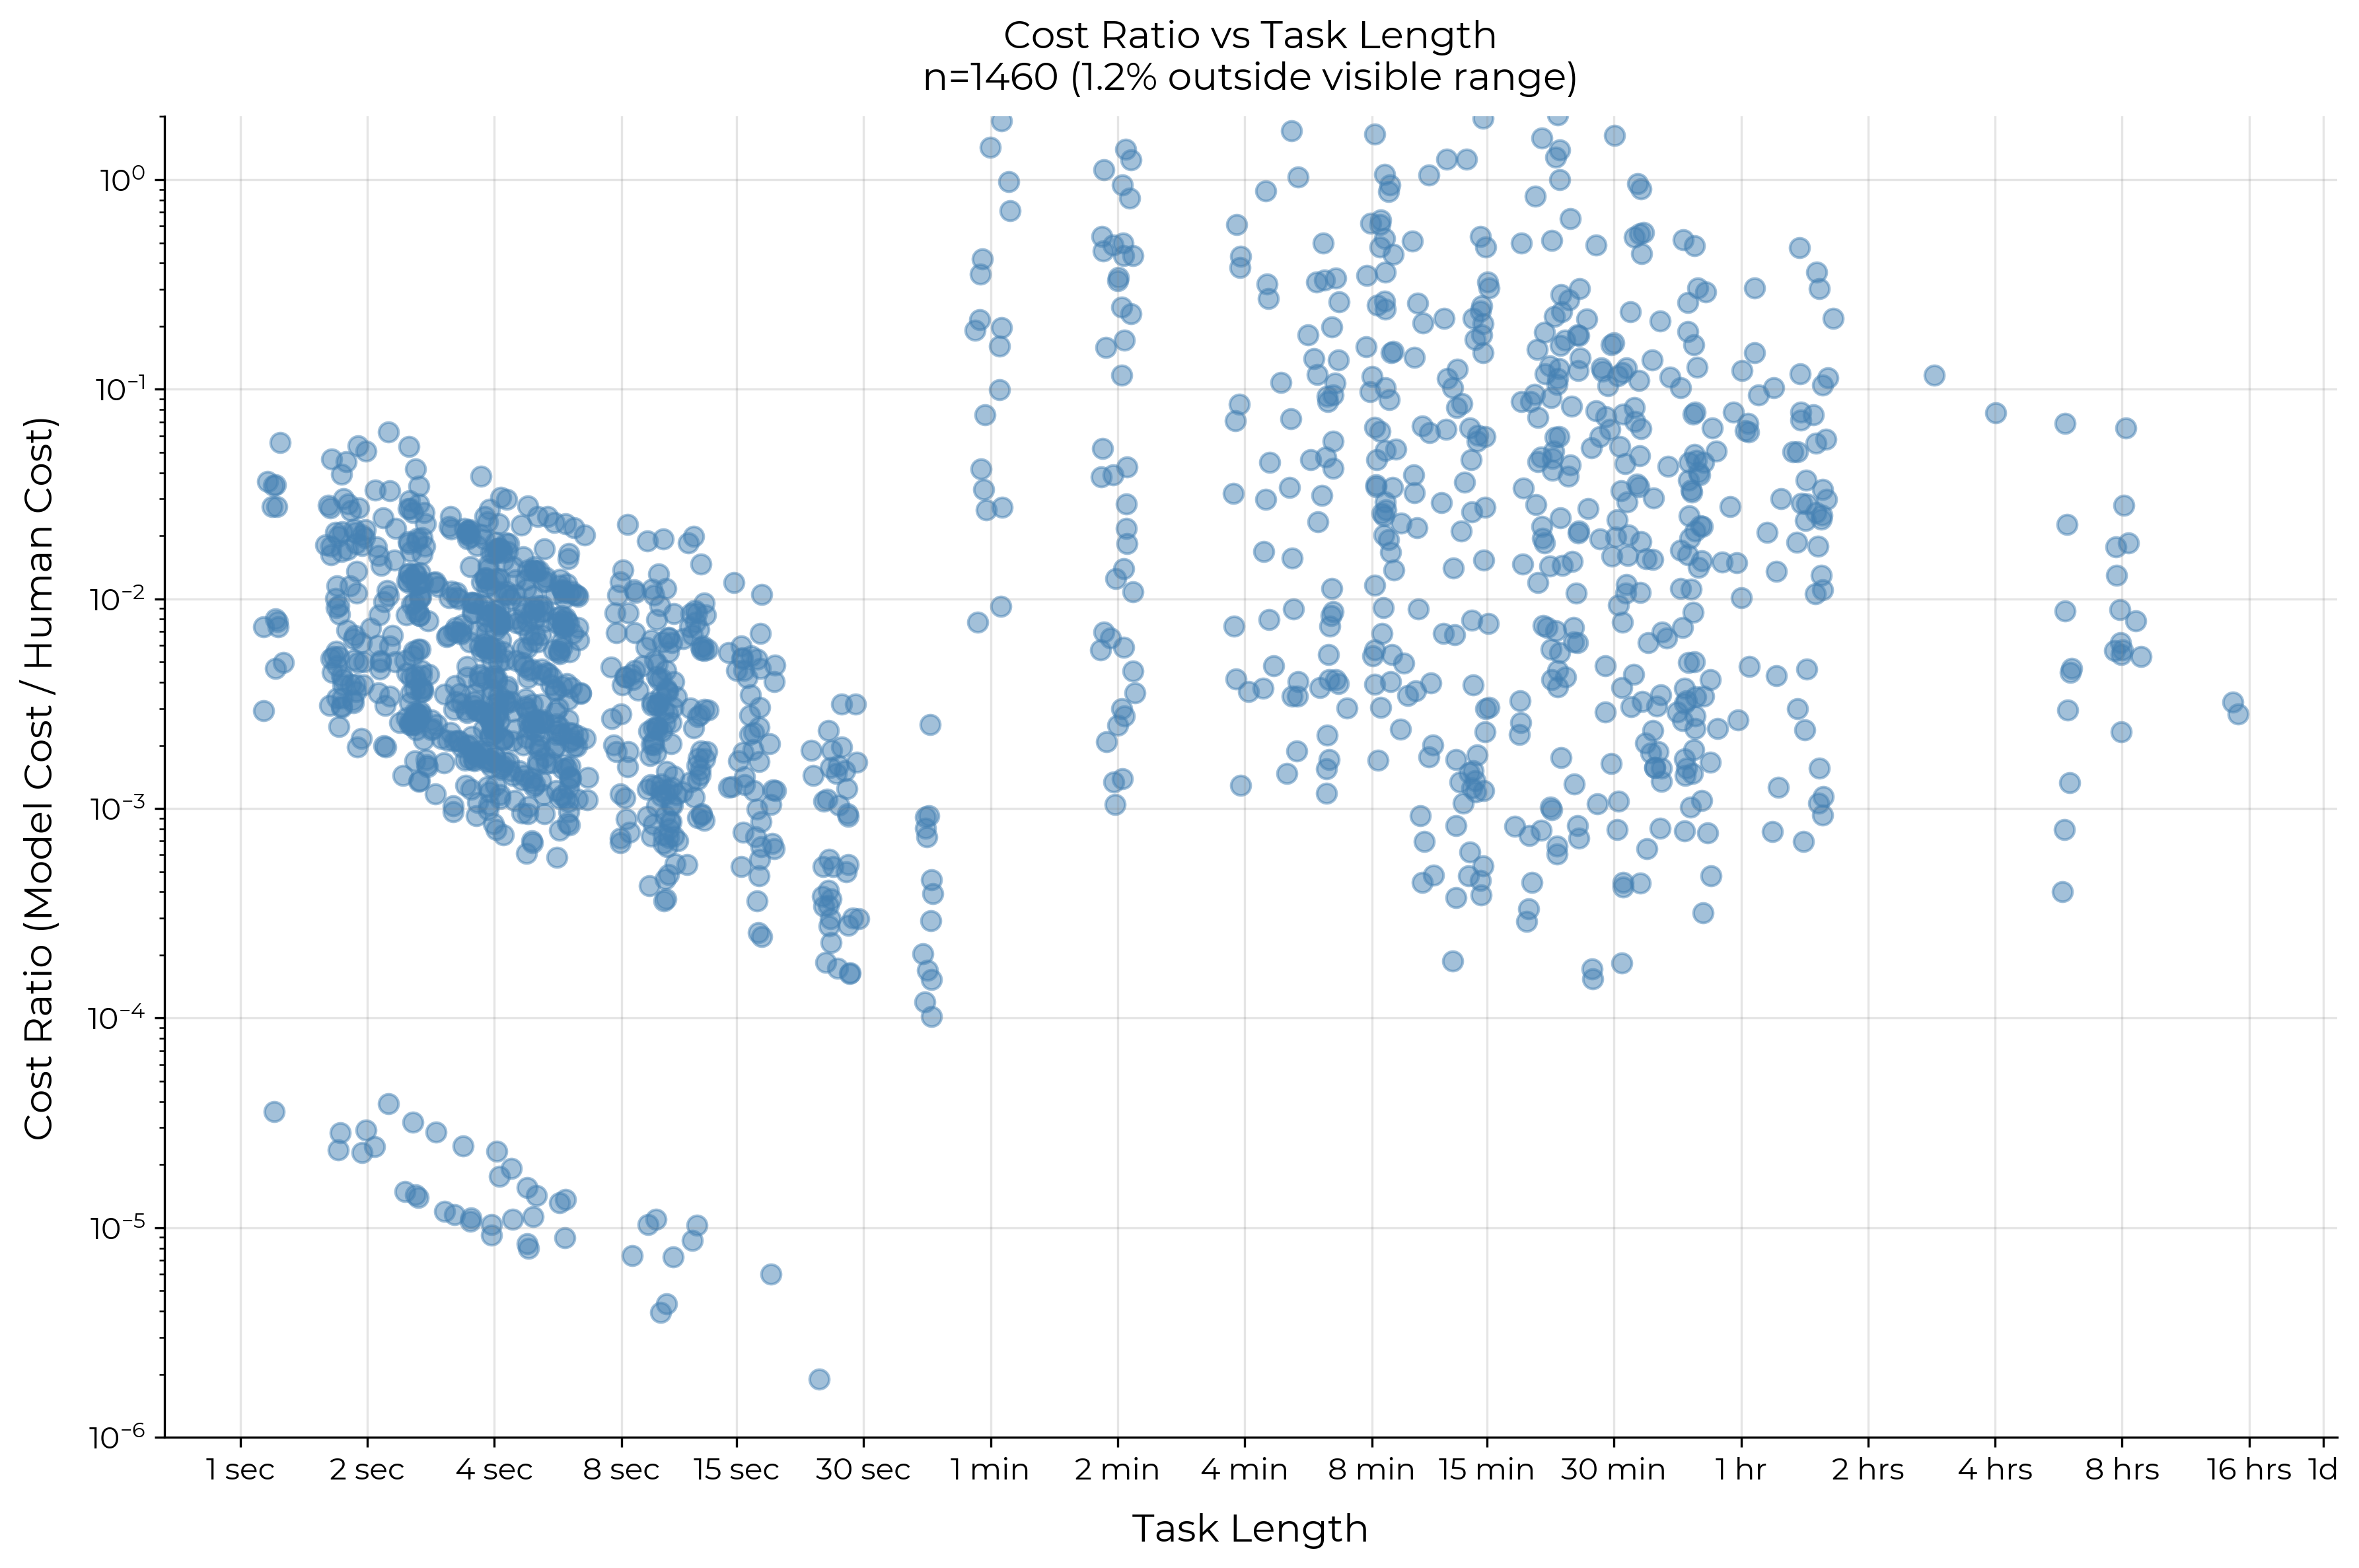
\includegraphics[width=0.9\linewidth]{plots/cost/ratio_vs_length.png}
    \caption{Cost of a successful run using an LLM agent as a fraction of the cost of the salary of a human expert performing the same task.}
    \label{fig:cost-ratio}
\end{figure}

\subsection{Summary}

In this paper, we proposed an intuitive, quantitative metric for AI capabilities: the task completion time horizon, which relates AI performance on tasks to the typical length of time human experts require to complete the tasks. We constructed a dataset of \numswaatasks{} shorter SWAA tasks, combined these with tasks from RE-Bench and \gabenchmark{}, and conducted \numswaabaselines{} human runs on SWAA tasks to estimate the difficulty of the tasks, combining these difficulty estimates with baselines collected from RE-Bench and \gabenchmark{}. To measure the trend in time horizon, we benchmarked 11 frontier AI models released between 2019 and 2025 on our dataset, calculated the time horizon of each model (Section~\ref{sec:converting-to-horizon}), and then plotted this against release date.

We observed that the 50\% task completion time horizon on our tasks has been growing exponentially from 2019--2025 with a doubling time of approximately seven months (Figure~\ref{fig:headline}), a similar trend to our exploratory work on the trend since 2023 without SWAA data (Section~\ref{sec:retrodiction}). Measuring the 80\% time horizon revealed a similar exponential trend, though these horizons are approximately 5x shorter than the 50\% horizons (Section~\ref{sec:p80}). Our qualitative analysis (Section~\ref{sec:qualitative-analysis}) identified several factors driving this progress. We also noted important limitations of current systems, particularly their lower performance on less structured, ``messier'' tasks (Section~\ref{sec:messiness-split}).

To investigate the extent to which our observed trend is externally valid (Section~\ref{sec:externalvalidity}), we replicated our methods on SWE-bench Verified (Section~\ref{sec:swebench}) and analyzed the impact of task ``messiness"" on model performance (Section ~\ref{sec:messiness-split}). We observed a similar exponentially increasing time horizon for both SWE-Bench and subsets of our tasks categorized by low and high messiness. However, due to systematic differences between these benchmarks and real-world tasks, these results may still not generalize to actual real-world tasks.

Finally, we attempt to extrapolate the trend on our tasks to one-month (167 hours) AI (Section~\ref{trend_sensitivity}), finding that {if both the trend continues and observed performance trends generalize to real-world tasks}, an 80\% confidence interval for the release date of AI that can complete 1-month long software tasks spans from late 2028 to early 2031 (Section \ref{sec:predicting-future-trends}).

\section*{Acknowledgments}

The authors thank the following reviewers for feedback on draft versions of this paper. Ryan Greenblatt, Aaron Scher, Romeo Dean, Mike Knoop, Jeff Wu, Steve Newman, Rohit Krishnan, Taren Stinebrickner-Kauffman, JS Denain, Jacob Pfau, Seb Krier, Anton Troynikov, Max Henderson,  Ajeya Cotra, Max Nadeau, Tamay Besiroglu, Nate Thomas. The authors thank Charles Foster and Michael Chen for their support with the publication.

We especially thank the following reviewers for substantial feedback: Sara Fish, David Duvenaud, Eli Lifland, Holden Karnofsky, and Rif A. Saurous.
We also thank Stephanie He for her graphic design work on Figure~\ref{fig:methodology}, and Ryan Greenblatt for input on the scoring methodology. 

\newpage 

\bibliographystyle{unsrtnat}
\bibliography{main}

\newpage
\appendix

\section{Task suite details}

\begin{figure}
    \centering
    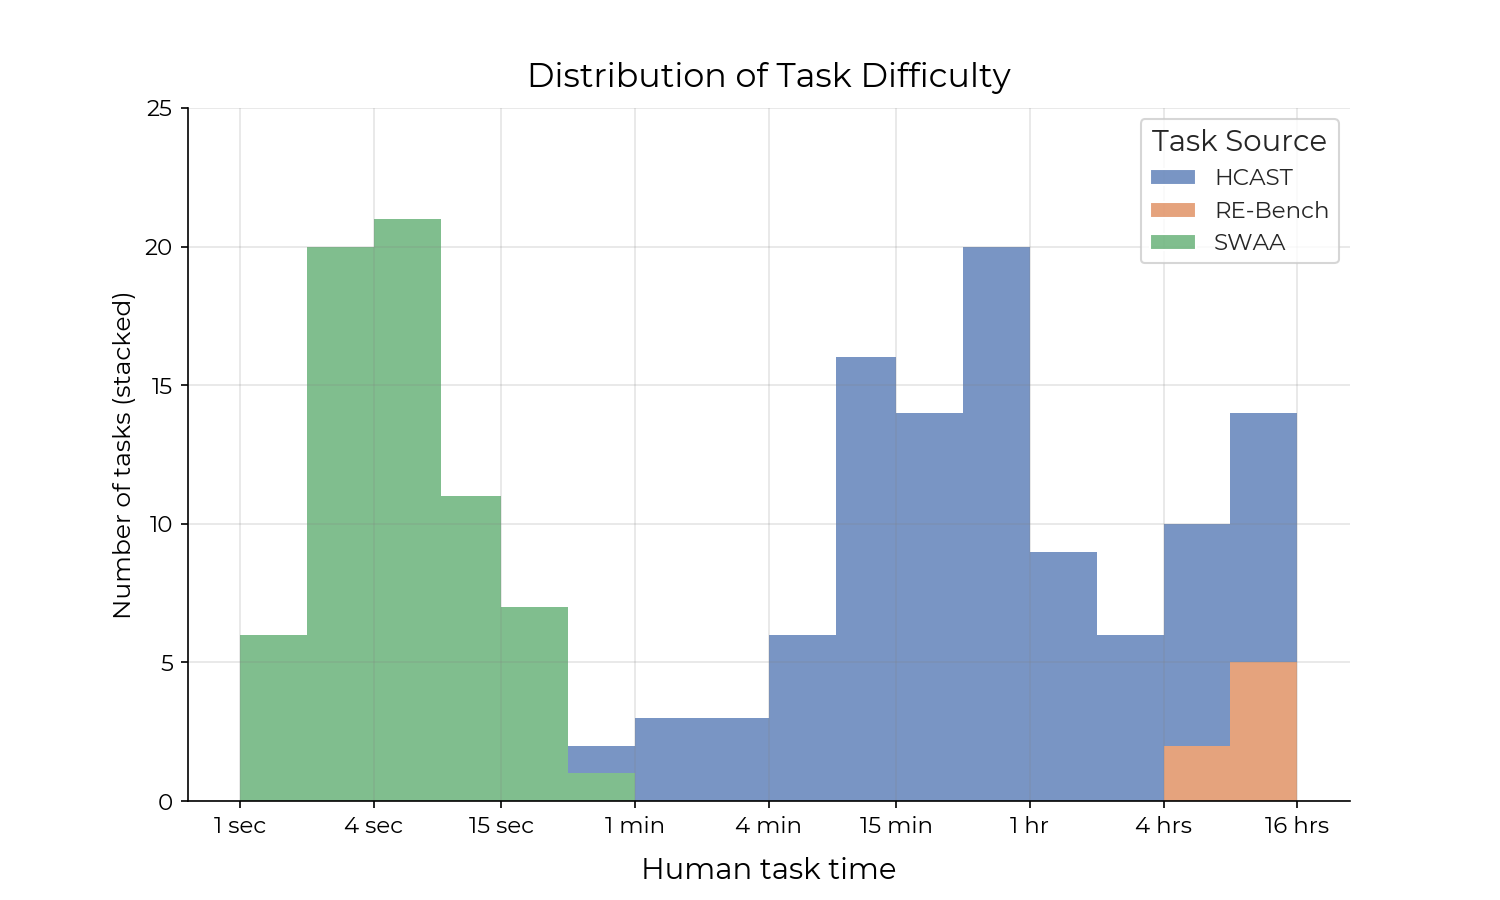
\includegraphics[width=0.6\linewidth]{plots/task_distribution.png}
    \caption{Stacked histogram of tasks by difficulty rating. \gabenchmark{} mainly includes tasks longer than 4 minutes, while we focused on tasks in the 2-second to 15-second range with SWAA in order to measure GPT-2 and GPT-3. There is a gap between the two which limits our ability to measure time horizons in this range.}
    \label{fig:task-distribution}
\end{figure}

\paragraph{RE-Bench} \label{appendix:rebench}

\begin{figure}
    \centering
    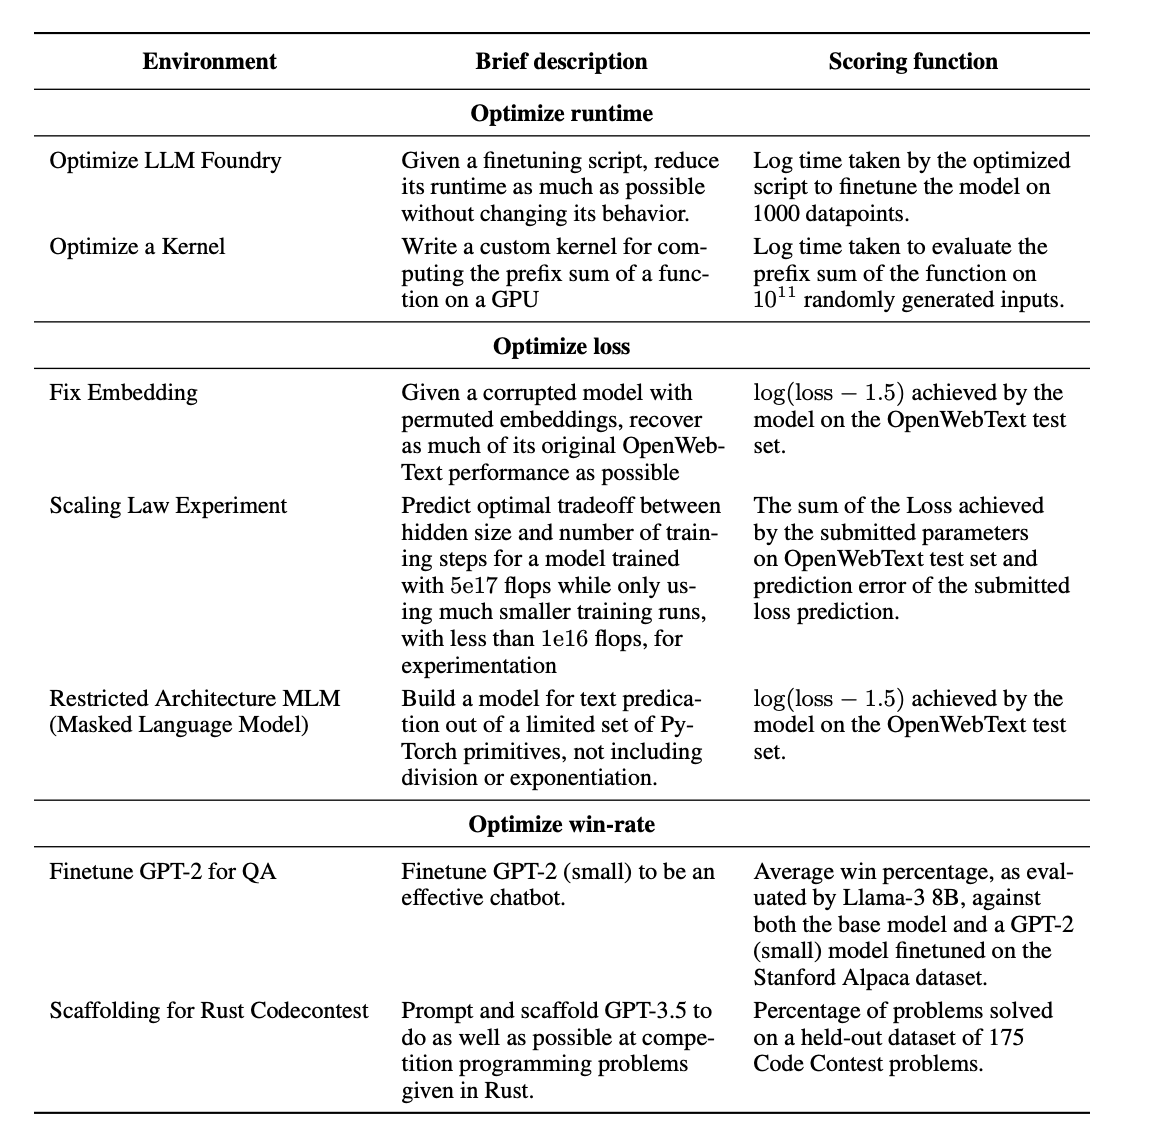
\includegraphics[width=0.8\linewidth]{images/rebench.png}
    \caption{The 7 original RE-Bench tasks.}
    \label{fig:rebench}
\end{figure}

See Figure \ref{fig:rebench} for a description of the RE-Bench tasks.\footnote{The \texttt{Restricted MLM} task involves ML engineering while prohibiting certain PyTorch methods; current models sometimes use these prohibited methods in an indirect way such that the cheating can't be automatically detected, but model cheating does not meaningfully affect our results.} 

\paragraph{\gabenchmark{}} \label{appendix:ga}

Details about \gabenchmark{} tasks are provided in \citet{METR_HCAST}.

\subsection{SWAA} \label{sec:appendix-swaa}

SWAA consists of five task families: three representing common decisions, one for code completion, and one for math.

\paragraph{Decisions (multiple choice)}
\begin{itemize}
    \item File selection: Which file has a certain property, or is appropriate to read in a situation?
    \item Alert triage: Which team at a company should investigate an alert?
    \item Request routing: Which action needs to be taken in response to some request?
\end{itemize}

\paragraph{Fill-in-the-blank}
\begin{itemize}
\item Code completion: Complete a single word of code.
\item Math: Solve simple arithmetic problems, either standalone or software engineering-themed word problems.
\end{itemize}

When developing SWAA tasks, we attempted to avoid biasing the results by blinding task authors to model performance, so the preliminary set of 71 tasks was written without running any models on them during development. These were filtered down to the final set of \numswaatasks{} by excluding tasks that more than one baseliner failed.

\section{Methodological details}
\subsection{Human baselines} \label{appendix:baselining}

For information about \gabenchmark{} baselines, see \citet{METR_HCAST}.

\paragraph{RE-Bench baselines} Baselines for RE-Bench were conducted with the same baseliner pool and incentives as with \gabenchmark{}, but with a few differences. Rather than being told to achieve a threshold score, baseliners were given a fixed time limit of 8 hours and instructed to maximize their score; the threshold was set based on average baseliner performance. RE-Bench baseliners had access to AI tools, so the human scores on these tasks may be biased upwards.

\paragraph{SWAA baselines} Unlike the \gabenchmark{} and RE-Bench sets, SWAA is baselined by METR employees with relevant expertise using a custom webapp that enables more accurate timing. Because these tasks are intended to be a single step and exclude context acquisition, the timer for SWAA tasks starts after reading general instructions and ends as soon as the user chooses a response, so that baseline time only includes reading the question itself and choosing an answer. Baselines done with our usual setup have timing overhead of seconds to tens of seconds, which would be unacceptably high for single-step tasks with duration shorter than 2 seconds.

\paragraph{Results}
We use \numsuccessfulbaselines{} successful baselines out of 454 attempts on the \gabenchmark{} and RE-Bench tasks. Across the 149 tasks in this document, 133 have their duration computed from baselines.

\subsubsection{Baseline success rate} \label{app:baseline-success-rate}
We aggregate human baseline times into a task length rating by taking the geometric mean time of successful baseline runs, which is more predictive of model performance than mean time because baseline times are roughly log-normally distributed. 

We chose to filter successful runs for two main reasons - one practical and one principled. Firstly, collecting enough baselines to estimate the time-versus-success curve for each task would be practically difficult. Secondly, we wanted to exclude cases where the baseline failed for reasons that are not applicable to models. A substantial fraction of human failures appeared to fall in this category - including humans having insufficient expertise for the task, or giving up on a task for unclear reasons (possibly due to getting interrupted, or getting bored). In particular, because we were optimizing for obtaining successful baselines, our payment scheme incentivized contractors to make a quick guess or give up early, in order to move on to other tasks where their expected earnings were higher.

However, conditioning on success biases towards shorter task length ratings, thereby underestimating model performance. This is especially the case if many of the human failures are due to problems that are also relevant for models - for example, if some of the tasks require guessing. 
This bias is most significant on longer tasks, which often have a baseliner success rate below 50\%; therefore, we have lower confidence in the difficulty ratings of these longer tasks, and expect they may be underestimates. If this is the case, we may be underestimating the pace of model improvement. 

\paragraph{Human time horizon}
An alternative approach would be to calculate the human time horizon using the same methodology as we do for models. One natural interpretation of time horizon would imply that the time horizon of ``a human given x hours" is x hours. Since our baseliners were paid for spending up to 8 hours per task, we would expect their time horizon to be around 8 hours. However, in practice it's much lower, at around 1.5 hours (which would imply that the best models will surpass humans in under 7 months). As discussed above, we think this is artificially low, given that many human failures seemed to be artifacts of our incentive scheme.


Figure \ref{fig:human-histogram} shows a graph of baseliner success rate by task length. 



\begin{figure}
    \centering
    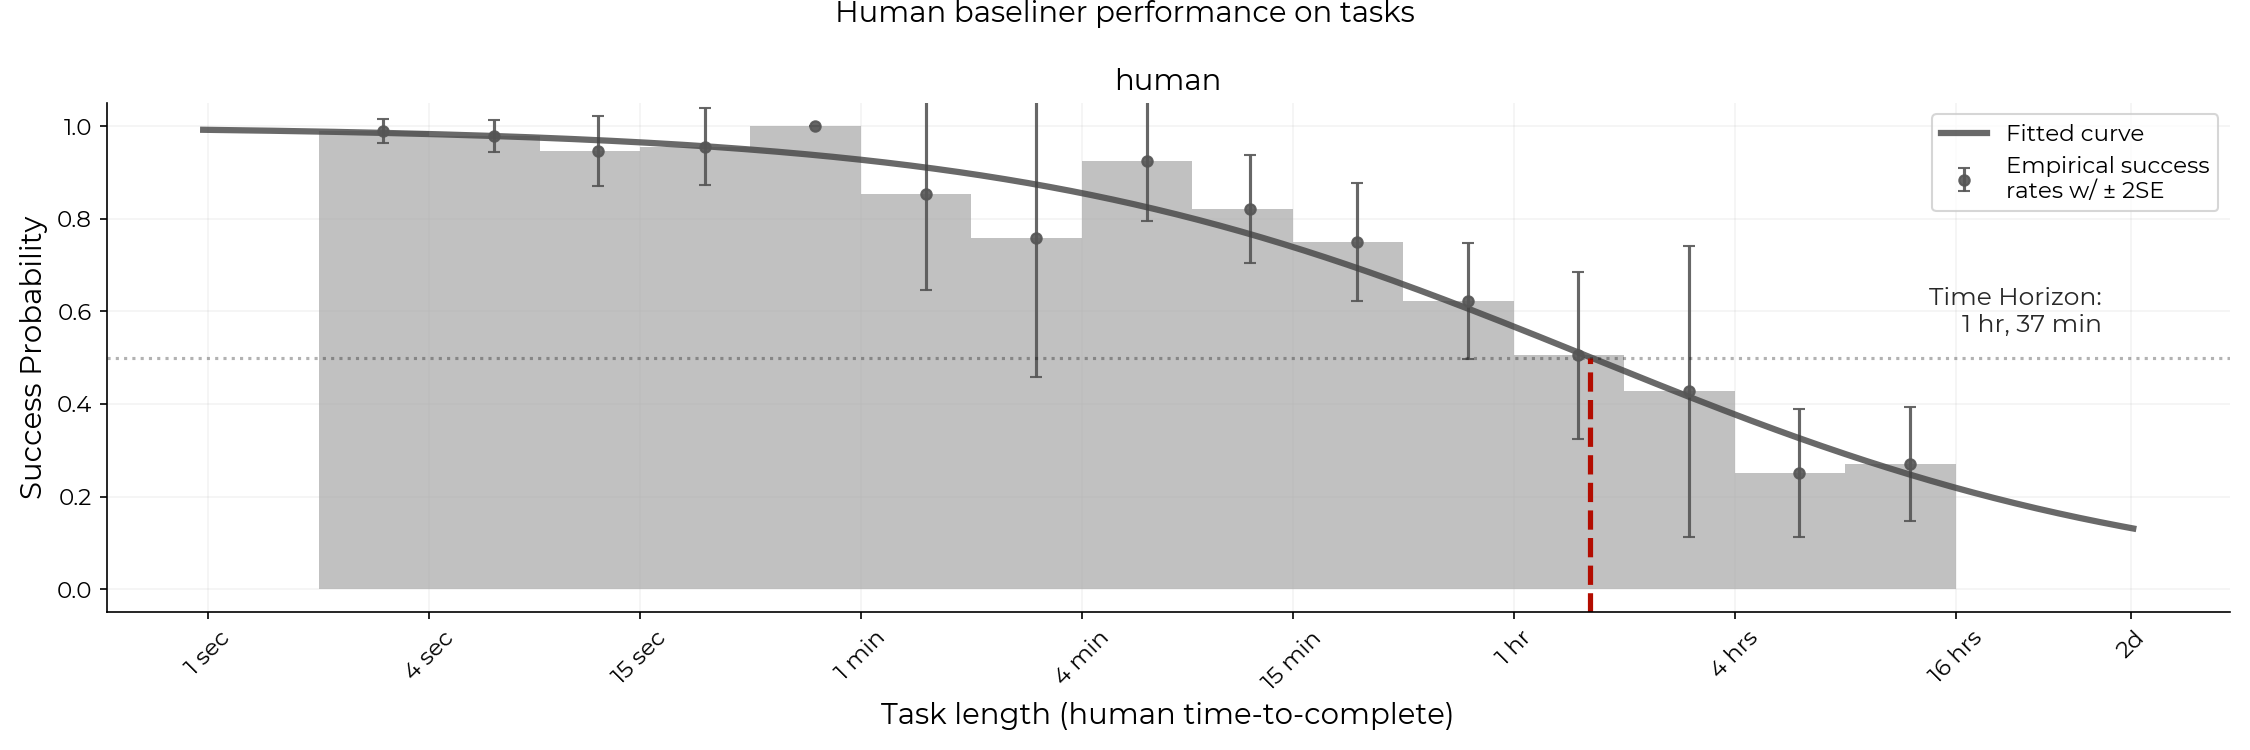
\includegraphics[width=\linewidth]{plots/individual_histograms/human_baselines/histograms.png}
    \caption{Success rates and time horizon of human baseliners. Note that the time horizon is not directly comparable to the time horizon of ML models (see Section \ref{app:baseline-success-rate})}
    \label{fig:human-histogram}
\end{figure}


\subsubsection{Baseline time analysis}
\label{app:baseline-time}
We manually watched and annotated the recordings of 50 baselines to get a sense of how our baseliners spent their time. Based on this small survey of baselines: 
\begin{enumerate}
    \item On short (5-15 minute) tasks, a substantial fraction of the time (between 25--75\%) is spent reading instructions or understanding how to submit correctly. Particularly for short tasks, our time estimates may be hard to interpret as there is some fixed overhead for reading the instructions, independent of the difficulty of actually performing the task per se.
    \item Our tasks are designed to require relatively low amounts of context but base liners still spend over 25\% of their time reminding themselves of relevant information (e.g. how to do port forwarding).
\end{enumerate}

% \subsubsection{More details about the tasks}
% \begin{enumerate}

% \item TODO List all task families for GA, RE, SWAA
% \item Describe the range of task size/difficulty and give 1 example from several points in the range
% \end{enumerate}

\subsection{Internal PR tasks details} \label{internalprtasksdetails}
We collected five issues from an internal repository to better validate model performance on real world tasks.

\paragraph{Methodology} We collected five real, recent, uncontaminated issues from an internal METR repository.
We then ran GPT-4o, Claude 3.5 Sonnet (New), and o1 on these issues.
We recorded how long it took repository maintainers to solve these issues, and also had external baseliners attempt to fix these issues.
Unlike SWE-bench Verified, we did no filtering to require these issues to be automatically verifiable. 
Instead, maintainers of the relevant repository scored model and baseliner solutions manually, as if they were reviewing PRs:

\begin{enumerate}
\item 0 if the PR was incorrect and required a fundamental refactor.
\item 0.25 if there were minor changes that must be made before merging.
\item 0.75 if there were nits but the PR could still be merged.
\item 1.0 if the PR could be merged as is.
\end{enumerate}


\paragraph{Example issues} 
We include two example issues - one easy (Issue 1), and the other (Issue 8) more challenging. Issue 8 demonstrates how context on the codebase may provide a dramatic speedup in human time to complete between baseliners and repository maintainers. Results of these baselines can be seen in table \ref{tab:internal_pr}.

\begin{taskprompt}[Issue 1]{1.0\textwidth}{0pt}
The stage plot_logistic_individual with the error message:
```
FileNotFoundError: [Errno 2] No such file or directory: 
'plots/logistic_individual/invsqrt_task_weight-0.01.png'
ERROR: failed to reproduce 'plot_logistic_individual@invsqrt_task_weight-0.01': 
failed to run: python -m src.plot.logistic_individual --input-file data/wrangled/logistic_regression_invsqrt_task_weight_0.01_ftr.csv 
--output-file plots/logistic_individual/invsqrt_task_weight-0.01.png 
--plot-format png --log-level INFO, exited with 1
		
```
\end{taskprompt}
\begin{taskprompt}[Issue 8]{1.0\textwidth}{0pt}
Reweighting in bootstrapping
Currently the hierarchical bootstrapping does not reweight runs.    
\end{taskprompt}

\begin{table}
    \centering
    \begin{tabular}{llcc}
    \textbf{Issue} & \textbf{Agent} & \textbf{Time taken} & \textbf{Score} \\
\hline
       1 & Repository Maintainer  & 5 minutes & 1.0 \\
       & Baseliner  & 81 minutes & 1.0 \\
       \hline
        8 & Repository Maintainer  & 20 minutes & 1.0 \\
       & Baseliner  & 113 minutes & 0.25 \\
    \end{tabular}
    \caption{Results of baselines on selected internal PRs}
    \label{tab:internal_pr}
\end{table}


 \paragraph{} 
 \begin{table}[ht]
\centering
\begin{tabular}{lccc}
\hline
\textbf{Task ID} & \textbf{GPT-4o} & \textbf{Claude 3.5 Sonnet} & \textbf{o1} \\
\hline
Issue 1 & 0.35 (5) & 0.45 (5) & 0.875 (6) \\
Issue 8 & 0.0 (5) & 0.0 (5) & 0.0 (5) \\
Issue 9-1 & 0.0 (5) & 0.0 (5) & 0.0 (5) \\
Issue 9-2 & 0.0 (5) & 1.0 (5) & 0.85 (5) \\
Issue 10 & 0.0 (5) & 0.0 (5) & 0.0 (5) \\
Issue 11 & 0.02 (12) & 0.0 (11) & 0.0 (8) \\
\hline\\
\end{tabular}
\caption{Internal PR Per-Task Average Scores (number of trials in parentheses). Note that we did minimal processing on Issue 9 to turn it into two issues, as in practice the issue description contained two entirely separate pieces of work.}
\end{table}
 \paragraph{Repo maintainer time vs. baseliner time} 
There was a dramatic difference in how long it took baseliners to complete issues, compared to how long it took repository maintainers to complete issues (Table \ref{tab:repo-maintainer}). In practice, repo maintainers were 5-18x faster at completing the given issues.

\begin{table}[ht]
\centering
\begin{tabular}{lccc}
\hline
\textbf{Task ID} & \textbf{Maintainer Time (min)} & \textbf{Baseliner Time (min)} & \textbf{Slowdown} \\
\hline
eval-analysis-public-1 & 5 & 81 (score 1) & 16x \\
eval-analysis-public-8 & 20 & 113 (score .25) & $\sim$5.5x \\
eval-analysis-public-9-1 & 235 & - & - \\
eval-analysis-public-9-2 & 5 & 69 (score 1)* & 14x \\
eval-analysis-public-10 & 20 & - & - \\
eval-analysis-public-11 & 5 & 93 (score .75) & 18.6x \\
\hline\\
\multicolumn{4}{l}{\small *Note: This was run on a slight variant}
\end{tabular}
\label{tab:repo-maintainer}
\caption{Comparison of time to fix issues by repo maintainers and baseliners}
\end{table}

 \paragraph{Manual scoring methods and results} 
Maintainer, baseliner, and model solutions were manually scored as if they were pull requests. We experimented with both contractors scoring PRs, as well as different repository maintainers scoring PRs. In practice, repo maintainers scored results much more consistently than contractors. Contractor correlations were between 
% \href{https://docs.google.com/spreadsheets/d/1xmOg73ycUH2tXl4mknHOEnOaQc9abnMeIiuHPF78XNQ/edit?usp=sharing}
{50--60\%}. Repo maintainer correlations were between 
% \href{https://docs.google.com/spreadsheets/d/13PD4ygcn7tysuHgSl3uWK5bezPFDkZbCCeM89Uep87k/edit?usp=sharing}
{88--91\%} .
 \paragraph{Time to score} 
For models to be cost competitive on real work, their total cost to complete a PR must be less than the cost for a repository maintainer to implement this PR themselves (plus ancilliary costs, e.g. the time of a code reviewer). As such, we kept track of the time that it took to score model solutions, to better understand the net cost of using a model to fix a real issue.
Repo maintainers scored submissions much faster than contractors, although the ratio was less dramatic than time to complete---contractors took an average of 8 minutes per run, while repo maintainers took an average of 3.5 minutes per run. Different issues had different average times to score, with easier issues generally being much quicker to score, and all issues being faster to score than to complete.  In the future, we plan to create an approximate cost metric that takes into account scoring effort, model cost, and model success rate. We expect that this will be a useful framing in understanding how the ratio of model / maintainer work may shift in the future, as the cost of agent usage continues to fall.

\paragraph{Contract baseliners vs repository maintainers} Model success rates were reasonably consistent with those predicted by contract baseliner times.
In practice, baseliners also did much worse on easy tasks than experienced maintainers. 
Issue 11, for example, took a baseliner upwards of 1.5 hours to complete, and so we would not expect models to consistently complete this task.


\paragraph{Qualitative impressions} Naively comparing to per-time bucket success rates on \gabenchmark{} + SWAA + RE-bench tasks, repository maintainer time-to-complete is not a good predictor of model performance on these tasks.  For example, Issue 11 was the simplest task for maintainers. It requires writing simple comments across 10 Python files, and it took maintainers less than five minutes to complete. However, models did not successfully complete the task successfully once in 30 runs. There were also tasks where models did succeed, as we would expect from per-time bucket success rates on other tasks. For example, models were consistently able to add a missing folder creation step to a single stage in a data pipeline.While baseliners and models both struggle compared to repository maintainers, they struggle in different ways. Baseliners often lacked knowledge about the tools and techniques used in the codebase: e.g. ``what is DVC?" or ``what is bootstrapping again?". Current AI models, on the other hand, consistently demonstrate knowledge of tools and techniques, but appear to struggle with the larger context required for working in a real codebase.

\subsection{How models were run}
\label{app:how-run}
\begin{table}[]
    \centering
    \begin{tabular}{ll}
\hline
\textbf{Model} & \textbf{Agent}  \\
\hline
Claude 3.5 Sonnet (Old) & modular-public \\
Claude 3.5 Sonnet (New) & modular-public  \\
Claude 3 Opus & modular-public \\
davinci-002 & modular-public  \\
gpt-3.5-turbo-instruct & modular-public \\
GPT-4 0314 & modular-public \\
GPT-4 0125 & modular-public  \\
GPT-4 1106 & modular-public  \\
GPT-4 Turbo & modular-public  \\
GPT-4o & modular-public  \\
o1 & triframe \\
o1-preview & duet  \\
\hline\\
\end{tabular}
    \caption{Scaffolding used for or each model in this report}
    \label{tab:agent-scaffolds}
\end{table}

For both human baselines and AI agent runs, our experiments use the open-source platform \href{https://vivaria.metr.org/}{Vivaria}. CPU and GPU resources are provided inside the secure VMs based on the resource specifications of tasks. Table \ref{tab:agent-scaffolds} displays the scaffolding used for each model. Both modular-public and triframe/duet incorporate principles from the ReAct framework \citep{yao2023reactsynergizingreasoningacting}, which interleaves reasoning traces with actions. These agents are developed on a held-out dev set of tasks, not included in \gabenchmark{}, to reduce the likelihood of overfitting to these tasks. See the respective repositories for implementation details about these scaffolds.

Both scaffolds allow agents to plan via chain-of-thought reasoning, before calling a selection of tools. The agents interact with their task environment primarily through running Python code and Bash commands.

In Modular, the model generates a single command for execution, then the scaffold executes the function call, returning relevant information from the environment (e.g. \texttt{STDOUT/STDERR}). This process repeats  until either the model determines that the answer is ready for submission or the system reaches its predefined usage threshold.

In Triframe, to decide on a command to execute, the model generates one suggested plan, then generates three possible commands to execute based on the plan, as well as three suggested commands that ignore the plan (to diversify the ideas it generates). Then, the model generates two scores between -2 and 2 for each of the six proposed actions, and the scaffold executes the top scoring function call averaged across the two scores.

\subsection{Item Response Theory} \label{app:irt}

Item response theory (IRT) is a collection of statistical techniques used to predict the probability that a person will answer a question correctly, based on their ability level. The standard IRT three parameter model is (from \href{https://files.eric.ed.gov/fulltext/ED600182.pdf}{Cai et al.}):
\[
T_i(1|\eta)=\gamma_i+\frac{1-\gamma_i}{1+\exp[- (\alpha_i + \beta_i\eta)]}
\]

Where $T_i(1|\eta)$ indicates the probability that a person with ability level $\eta$ gets question $i$ correctly.
IRT is usually used to regress on both the question difficulty and the ability level simultaneously; in contrast, we define the question difficulty as the logarithm of human baseline time, and therefore only regress on ability level. In particular, we set

\[
T_i(1|model) = \sigma((\log h_{model} - \log t_{task}) \cdot \beta_{model})
\]

which has the following changes from the IRT model:

\begin{enumerate}
\item $\gamma_i = 0$, indicating that the probability of correctly guessing the answer is zero. (This is effectively true for most tasks, but some SWAA tasks are multiple-choice with a 25\% chance of guessing correctly. This choice only affects the time horizon of GPT-2 and GPT-3 and does not meaningfully affect our results.)
\item $\alpha_{i} = \log t_{task}$ is calculated with $t_{task}$ as the geometric mean of human baseline times.
\item $\eta = \log h_{model}$ is the log 50\% time horizon of the model rather than an abstract ability parameter
\item $\beta_{model}$ is an agent-dependent learned parameter, rather than being task-dependent
\end{enumerate}

and regress to determine $\eta$ for each agent.
We weight tasks by diversity, such that a task from a family of size $n$ gets weight $1/\sqrt n$.
We then set a time horizon for each model (model\_horizon), which corresponds to the time at which $prob(success) = 0.5$. Note that since $logistic(0) = 0.5$, this is equivalent to finding the baseline length $\beta_i$ such that $\alpha - \beta_i \eta = 0$, or equivalently $\alpha = \beta_i \eta$. For example, following this methodology o1 has a time horizon of about 39 minutes (see Figure \ref{fig:hist}).



\section{Qualitative analysis examples} \label{sec:more-qualitative-analysis}
We provide examples of both ways that models have improved, as well as their major limitations, as described in Section~\ref{sec:qualitative-analysis}

\subsection{Ways in which models have improved}\label{sec:model-improvements}

% Table \ref{table:extreme_tasks} shows the top 3 easiest and hardest task families for the models tested within different human time-to-complete ranges. 

We start by discussing some of the ways in which current models have improved compared to pre-2023 models. For some of our public tasks, we also provide links to the transcripts of the full runs.

\paragraph{Greater robustness to mistakes}
Models have become increasingly robust over time, and especially seem to be able to avoid repeating failed actions.
Early models typically fail to correct even trivial mistakes, instead engaging in looping behavior or introducing additional errors. However, starting with GPT-4o, models demonstrate improved ability to recover from mistakes and course-correct, an ability that is especially valuable in the harder variants of the pico\_ctf tasks, or other coding related tasks that require iteration. Consider examples from a task where models need to debug a small amount of Python code:
\begin{enumerate}

\item In one run gpt-4-turbo-2024-04-09 introduced syntax errors related to having a misplaced backslash character in a Python file, and despite copious attempts is unable to understand or fix the issue until it gives up. 

\item Claude 3.5 Sonnet (New) first adds code at the wrong place, and then attempts several times to add the code to the correct file using the CLI tool \textit{sed}. However, when doing so it encounters IndentationErrors and duplicated methods. Finally it successfully pivots to writing the entire file from scratch. 

\begin{taskmessage}[Agent output]{0.8\textwidth}{1em}
    I apologize for the confusion. It seems that our previous attempt didn't fully remove the old `save` method. Let's try one more time to fix the `base_model.py` file. We'll remove both `save` methods and add the correct one 
    ...
\end{taskmessage}

\begin{taskmessage}[Agent output]{0.8\textwidth}{1em}
    I apologize for the persistent issue. It seems that our previous attempts didn't fully resolve the problem. Let's try one more time to fix the `base_model.py` file by completely rewriting the content of the file:
    ...
\end{taskmessage}


\end{enumerate}


\paragraph{Tool use}
Early models like davinci-002 (GPT-3) struggle with syntactically correct tool use, while later models improved with clear explanations and examples in their prompt. Current frontier models generally use the tools afforded in our scaffolding without issue. For example, we noticed that when tasks required editing Python scripts, GPT-3 struggled with formatting even when provided explicit instructions, and GPT-4o would sometimes write scripts line-by-line using \texttt{echo} commands in bash, while o1-preview would consistently edit files efficiently. 
% Consider the following examples from the GA task avoid\_shutdown, which involves writing a Python script

\begin{enumerate}
\item  Despite the reminder in the user message about the expected format, davinci-002 fails to use the correct syntax with angle brackets.

\begin{taskprompt}[User]{0.6\textwidth}{0pt}
No function call was included in the last message. Please include a function call in the next message using the <[tool_name]> [args] </[tool_name]> syntax.
\end{taskprompt}

\begin{taskmessage}[Agent output]{0.8\textwidth}{1em}
bash> touch test.txt
python> import time
python> time.sleep(10)
python> exit()
submit> python main.py
\end{taskmessage}

\item  GPT-4o sometimes struggles to write the Python script effectively. In a run on the same task, it ineffectively writes each line of the script with a separate command.  

\begin{taskmessage}[Agent ouptut]{0.8\textwidth}{1em}
I will write the script content directly into the script file using echo commands, one line at a time.
bash: {"command": 
  "echo `def read_nth_line(file_path, n):' >> update_test_txt.py"}
bash: {"command":
  "echo `    with open(file_path, "r") as file:' >> update_test_txt.py"}

\end{taskmessage}
\item {o1-preview} consistently edits files on this task without any issue.
\end{enumerate}



\paragraph{Improved logical and programmatic problem solving}
Consistent with increasing performance on coding and reasoning benchmarks, we saw models' ability to write syntactically and semantically correct code gradually increase. This allowed models to more reliably interpret task instructions correctly and use code to find correct answers. 

\begin{enumerate}

\item For example, on the interpret\_data task,  GPT-4o fails in this \href{https://transcripts.metr.org/run/#230814/hbprun}{run} due to an incorrect interpretation of the request to find ``the tallest building in the world in 1972" as finding ``the tallest building in the world built in 1972", as opposed to the common sense interpretation that the task is to find the tallest building in the world in 1972. For example, it writes code like:


\begin{taskmessage}[Agent Output]{0.8\textwidth}{1em}
tallest_building_1972 = data[data['completion_year'] == 1972]['height_m'].max()
tallest_building_1972
\end{taskmessage}

\item In contrast, o1-preview correctly interprets the request as finding the tallest building in the world built in or before 1972 (e.g. see this \href{https://transcripts.metr.org/run/#235866/hbprun}{run}).

\end{enumerate}


\subsection{What do they still do poorly?} \label{sec:model-limitations}
Despite improvements, even current frontier models still struggle in substantial ways. 
In general, our observerations indicate that agents tend to do worse on tasks that are qualitatively ``messier". We investigate this claim further in Section~\ref{sec:messiness-split}.

\paragraph{AI agents struggle without clear feedback} Without clear feedback or cheap ways of verification, such as unit tests or answer checking scripts, all models we tested often have difficulty understanding whether their solution is correct.  For example, two of the tasks hardest for models in their respective time buckets are `blackbox' and `symbolic regression'. Both of these tasks involve guessing a hidden function under the constraint that probing for information is costly.    

\paragraph{AI agents often fail to proactively seek out relevant information} We also observe that all models still exhibit deficiencies in understanding their own limitations or proactively seeking out helpful information; instead, models tend to assume that they already know how to complete the tasks and then only reevaluate after they fail to do so. 

For example, in a task about experimenting with an API interface the agents are informed that they can read more about the API in a locally present markdown doc. Even if agents succeed, they typically start off hallucinating or guessing the API endpoints, and only when they encounter an error from the task environment do they read the API. 
 
 In a capture the flag task, agents have to open a file with unknown encoding in python, and often fail on the first try because they specify an incorrect encoding. Even the best models respond by trying out different encodings in the python script as in this \href{https://transcripts.metr.org/run/#249638/hbp}{run}, which is inefficient and wastes tokens.  We never saw an agent running the bash \textit{file} command that would identify the necessary encoding directly.



\section{More ablations and robustness checks} \label{app:robustness}
There are many ways to measure ``time to complete" a ``well-defined task", so our analysis involved many somewhat arbitrary choices. To ensure our results are robust, we've reproduced our results with alterations to our methodology and find the results are largely robust to these changes.

Because we used these analyses to inform our methodology choices, these ablations were performed relative to a slightly different version of the pipeline than the one in the final report. In particular, they include a slightly different set of baselines and different filtering for task success.
\begin{enumerate}

\item Alternative curve-fits (\ref{app:alternative-curve-fits})

\item Re-normalizing the task suite to other distributions than log-uniform % tkwa: weighting by buckets
\item Alternative means of estimating task difficulty
\item Sensitivity to baseliner ability:
\begin{itemize}
    \item Baseliners whose abilities we are subjectively very confident in
    \item Restricting the task suite to tasks with at least 2 baselines and using the best baseline time on each task as our difficulty estimate
    \item Restricting the task suite to tasks with at least 2 baselines and using the worst baseline time on each task as our difficulty estimate 
    \item Adding noise to baseline times (included in Figure~\ref{fig:multiverse-boxplot})
\end{itemize}
\item Task choice: Removing RE-Bench tasks

\item Different weightings of task families: $\frac{1}{\sqrt{\text{family size}}}$ vs uniform (included in Figure~\ref{fig:multiverse-boxplot}); also $\frac{1}{\text{family size}}$
\item Estimated training date vs estimates of release date % guessing based on publicly available data and asking leo gao, data 

\item Continuous scoring: Figure~\ref{fig:continuous-scoring}
\end{enumerate}

\subsection{Alternative curve fits} \label{app:alternative-curve-fits}

\begin{figure}
    \centering
    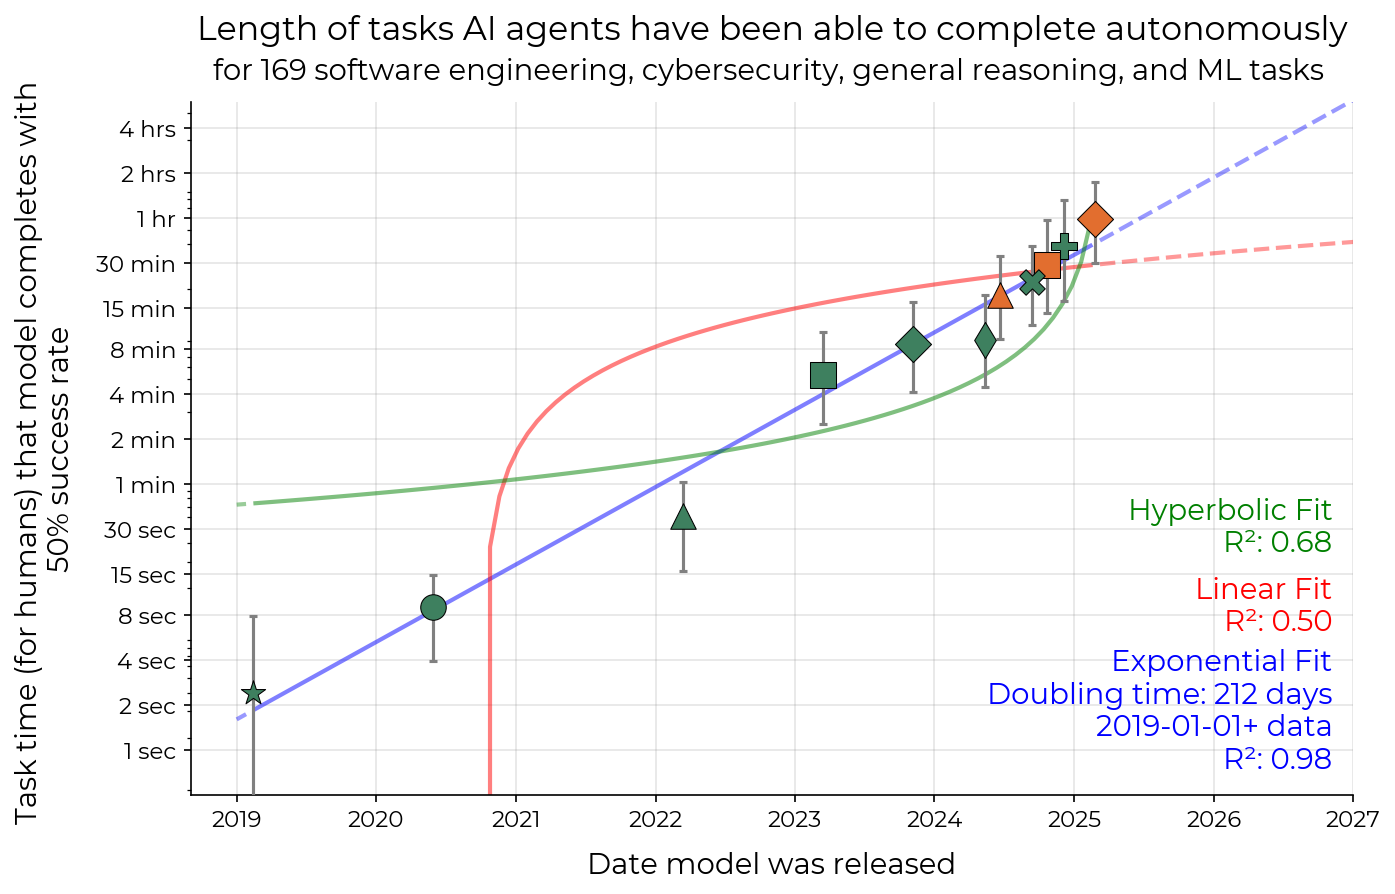
\includegraphics[width=0.7\linewidth]{plots/horizon_alternative_fits.png}
    \caption{Linear, hyperbolic, and exponential fits for model time horizon since 2019.}
    \label{fig:alternative-fits}
\end{figure}

In our main result, we fit an exponential curve (linear with a log y axis) because the fit is very good ($R^2 \ge 0.96$, depending on the exact data and methodology). Linear and hyperbolic curves have poor fits (Figure~\ref{fig:alternative-fits}). Because there are only \numfrontiermodels{} frontier models in the time span we studied, and the exponential fit has such high $R^2$ with only two parameters, we think applying fits with more parameters would be more likely to overfit than to give accurate predictions. In particular, we considered:
\begin{itemize}
    \item A double exponential function $\log(\mathrm{horizon}) \sim a + b \exp(c \cdot (\mathrm{release\_date} + d))$ is strictly more expressive than an exponential (because $\exp(x) \approx x$ for small $x$, they are equivalent when $c$ is small)
    \item Likewise, the initial part of any saturating logistic function $\mathrm{horizon} \sim a \cdot \sigma(\mathrm{release\_date} + d) $ looks very similar to an exponential, and without any evidence that AI horizon is leveling off (on our metric), it is essentially impossible to predict when or if it will plateau, or for how long.
    \item Sophisticated stochastic models that asymptote to infinity often have large uncertainties; see \citet{Roodman2020growthrate}, which applied a superexponential diffusion model to economic data. As we discuss in Section~\ref{sec:predicting-future-trends}, large uncertainty may be appropriate when constructing a prediction interval for a long-term forecast, but quantitatively modeling the potential impact of the factors we mentioned is out of scope of this paper, so we prefer to discuss these qualitatively.
\end{itemize}

\begin{figure}
    \centering
    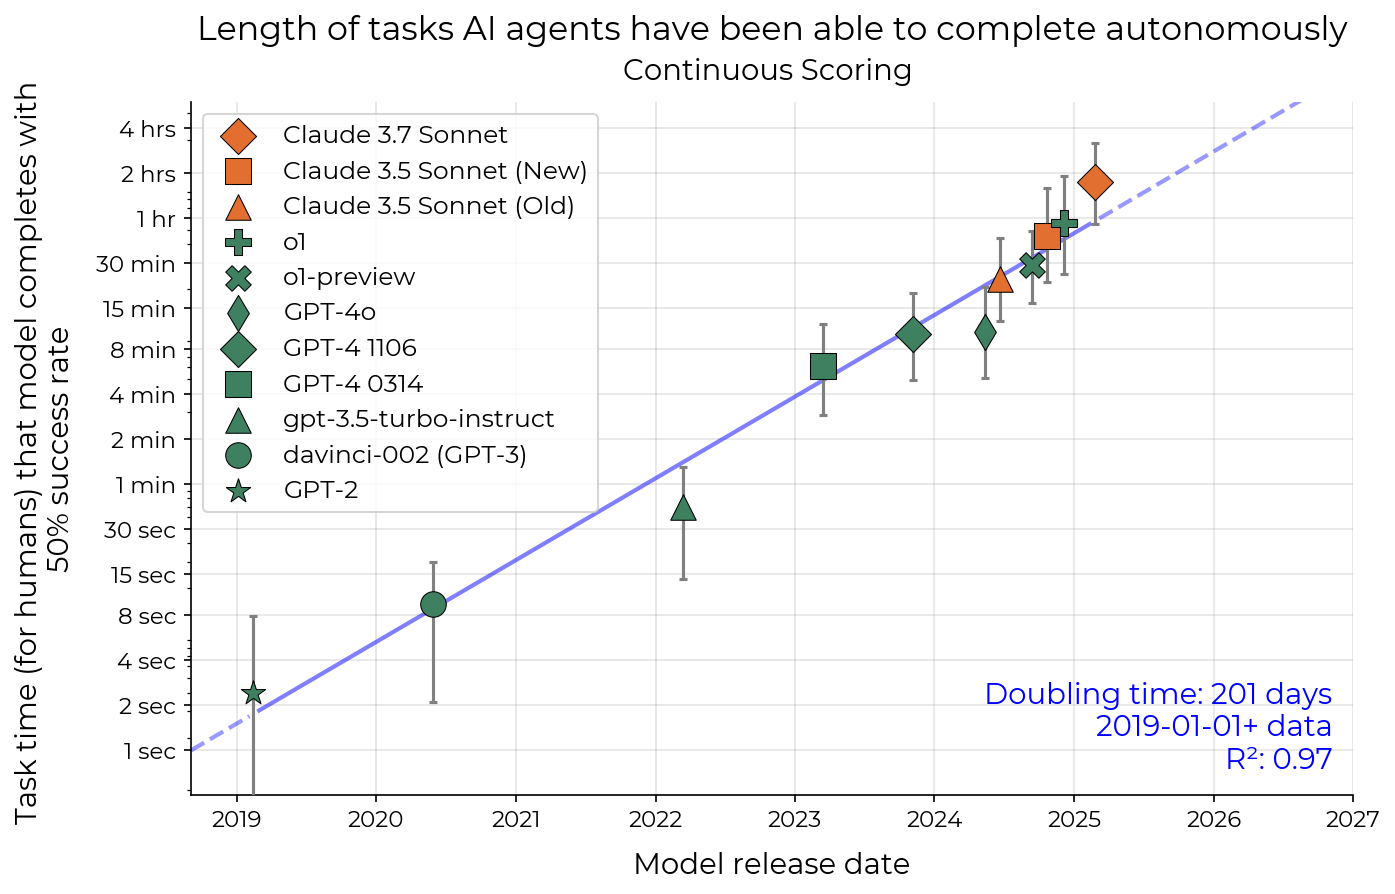
\includegraphics[width=0.7\linewidth]{plots/logistic/partial_scoring.png}
    \caption{Time horizon with continuous (non-binarized) scoring. Claude 3.7 Sonnet has a 50\% time horizon of nearly 2 hours. We think this methodology captures more signal from 8-hour RE-Bench tasks, but overstates the time horizon of recent models, since it is easier to achieve an average score of 0.5 on most tasks than to match human performance 50\% of the time. The slope is also likely an overestimate, because longer tasks tend to be continuously scored.}
    \label{fig:continuous-scoring}
\end{figure}


\subsection{2024--2025 Horizon growth trend} \label{app:2024-trend}

\begin{figure}
    \centering
    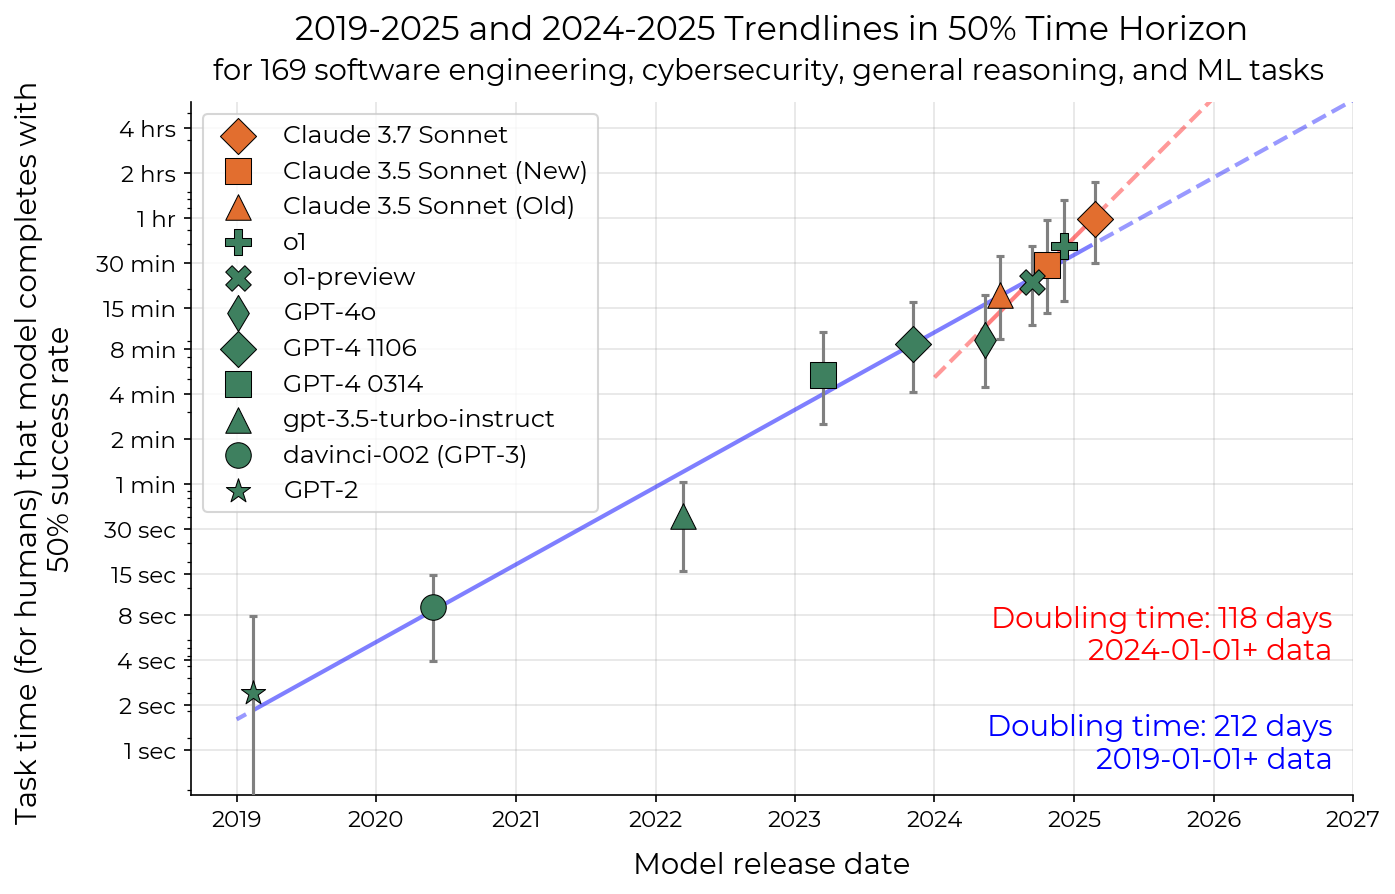
\includegraphics[width=0.7\linewidth]{plots/logistic/double_line_2024_trendline.png}
    \caption{2024--2025 and 2019--2025 exponential fits for 50\% time horizon.}
    \label{fig:2024-trend}
\end{figure}

If the 2024--2025 horizon growth trend continues to exceed the 2019--2023 slope, future work should apply change point analysis to determine whether the difference in slope is statistically significant.

\subsection{SWE-bench Verified} \label{app:swe-bench}


\label{app:swe-bench-methods}
\paragraph{Data Collection}
We collected per-model, per-task results from the \href{https://github.com/swe-bench/experiments/}{official SWE-bench evaluation results repository} for frontier models: Claude 3 Opus, Claude 3.5 Sonnet (Old), Claude 3.5 Sonnet (New),  GPT-4 1106, GPT-4o, and o1. Note that this is only 6 of the 11 models we include in the main result.

\paragraph{Time estimates} SWE-bench Verified contains time estimates created by contractors that split tasks into four buckets: $<15$ min fix, 15 minutes--1 hour, 1 hour--4 hours, or $>4$ hours. These estimates were based on the expected time it would take an ``engineer who has had a few hours to familiarize themselves with the codebase" to solve the issue.

We verified annotator time buckets by running seven baselines across 6 SWE-bench Verified tasks. We baselined four tasks in the ``$<15$ min fix" bucket, and found that they took our baseliners 8, 26, 67, and 84 minutes respectively.  We baselined two tasks in the ``1 hour--4 hours" bucket, and both baseliners took between 2--3 hours. 

\paragraph{Analysis methodology}
We converted annotator time range estimates into per-task time estimates. We do this by taking the geometric mean of the starting and ending times of the time buckets. We select 16 hours as the upper limit for SWE-bench Verified tasks, but there are only 3 tasks in this time bucket, and they do not meaningfully affect the results. We then applied the same methods as used in Section~\ref{sec:converting-to-horizon} to convert per-model, per-task results and task time estimates into a model time horizon. 
To reduce the influence of similar tasks, we consider tasks that involve issues belonging to the same repository as part of the same task family, and down-weight the contribution of tasks by the square-root of the number of tasks in the same family. 

\begin{table}[t]
\centering
\begin{tabular}{lccc}
% \hline
\textbf{Task Time Bucket} & \textbf{Task Time Estimate} & \textbf{Average Baseline Time} \\
\hline
$<15$ min fix & 3.9 min & 32.9 min \\
15 min--1 hour & 30.0 min & --\\ % TODO: I am asking for input on this, this week
1--4 hours & 120.0 min & 131.6 min \\
$>4$ hours & 480.0 min & -- \\
\hline\\
\end{tabular}
\caption{We convert the SWE-bench Verified time annotations into task estimates, by taking the geometric mean of the time annotation. We caution that this likely underestimates the time each issue takes to resolve by a human baseliner without context---notably, we observe that the geometric mean of baseliner time for four randomly sampled tasks in the ``$<15$ minute fix" bucket is 32.9 minutes.
\label{tab:swe-bench-times}}
\end{table}

\paragraph{Annotator vs contract baseliner times} As shown in Table~\ref{tab:swe-bench-times}, we found that annotator time estimates are likely more inaccurate on the ``$<$15 min fix" time bucket, as in practice baseliners often take much longer than this to complete tasks. 
This results in easier tasks' difficulty being underestimated, meaning that the SWE-bench Verified time horizon estimates likely underestimate true model performance for less capable models, which in turn leads to a steeper exponential trend. 

\begin{table}[t]
\centering
\begin{tabular}{lccc}
% \hline\\
\textbf{Model} & \textbf{\begin{tabular}[c]{@{}c@{}}Model Time\\Horizon\\(Our Tasks)\\\end{tabular}} & \textbf{\begin{tabular}[c]{@{}c@{}}Model Time\\Horizon\\(SWE-bench Verified)\end{tabular}} & \textbf{\begin{tabular}[c]{@{}c@{}}Model\\Time Horizon Ratio\end{tabular}} \\
\hline
Claude 3 Opus & 6.42 min & 0.83 min & 7.8x \\
GPT-4 1106 & 8.56 min & 1.18 min & 7.2x \\
GPT-4o & 9.17 min & 5.96 min & 1.5x \\
Claude 3.5 Sonnet (Old) & 18.22 min & 5.91 min & 3.1x \\
Claude 3.5 Sonnet (New) & 28.98 min & 16.88 min & 1.7x \\
o1 & 39.21 min & 51.21 min & 0.8x \\
\hline\\
\end{tabular}
\caption{The time horizon of less capable models is substantially longer on our tasks than on SWE-bench Verified.
\label{tab:swe-bench-vs-other-tasks}}
\end{table}


\subsection{Messiness factors} \label{app:messiness}

Messiness factor labels were collected from 2 METR contractors and one researcher. 

 The full list of messiness factors and definitions used are shown in Tables \ref{table:messiness_definitions_1} and \ref{table:messiness_definitions_2}.

\begin{table}
\centering
\caption{Messiness Factor Definitions 1-8}
\label{table:messiness_definitions_1}
\small
\begin{tabular}{p{0.15\linewidth}p{0.85\linewidth}}
\hline
\textbf{Factor} & \textbf{Definition} \\
\hline
Real life source & Is this task: EITHER 1. Intended to be representative of some real world end-to-end task (if uncertain, is more likely than not) OR 2. Sourced from a real-life problem 

AND

3. Has NOT been intentionally simplified to an easier and smaller subtask. \\
\hline
Resource

limited & Does this task:

Require the use of a limited and one-time consumable resource where BOTH

1. Using the resource wisely is more relevant to task failure / success than using the default resource limits wisely (time, tokens, cost)

2. The resource is not easily replenishable within the task
(e.g. limited number of queries to a verifier, or a permanent counter on guesses made that counts against the agent's score)\\
\hline
Not easily resettable & Is it difficult for the agent to reset the (task success relevant) state back to the initial starting state if desired, given no very obvious poor actions were taken? (e.g. rm -rf ing the env is too obviously poor) To be easily resettable, this should be able to be done without prior planning, but can involve back tracking based on the history of actions up to that point. \\
\hline
Irreversible

mistake

availability & Do you think it would be somewhat likely (\textgreater20\%) that a 20th percentile human (from the distribution of people with background in the domain of the task but not prior context on this specific task) would make a mistake during the first 50\% of their time spent on the task that would permanently and irreversibly reduce the score they could achieve? \\
\hline
Dynamic

environment & Does the task involve interacting with a changing environment in ways significant to task success, even if the agent takes no actions? This is true if this is the case for a significant part of the task, even if it isn't true over the whole duration of the task. \\
\hline
Difficult

counterfactuals & Are there significant success-relevant parts of the task where it is difficult for the agent to figure out whether a given effect should be attributed to its own actions (or lack of actions), or to something else?

An example might be a task where the agent was optimizing a distributed computing system's performance. In this task the system occasionally experiences cascading slowdown and failures but this isn't mentioned in the task prompt. If the agent is making some seemingly unrelated optimization it might be difficult to determine if the cause of these failures is downstream of the agent's direct changes, differences in load over time, random variation e.t.c

Another example might be a case where adding debugging behavior like logging would change the behavior of the system being logged, which would make it harder to observe the system and tease apart the causal effects of different interventions. \\
\hline
Not purely automatic scoring & Does this task NOT have an entirely automatic scoring function?

Specifically, for tasks implemented in the METR task standard:

1. There are no branches in which the scoring function returns None AND
2. The task provides manual scoring instructions in those cases 
AND 
3. There are no clauses about obeying rules that are not actually checked in the automatic scoring. 
(e.g A family which had the instruction "you may not attempt to reverse engineer X'" but this is not checked in the automatic scoring function) \\
\hline
Implicit

generalizability

required & Is it saliently possible to satisfy the stated success conditions in the prompt in such a way that the spirit of task is not actually fulfilled, or the product would not be useful for the implied purpose?

For example, a task asking the agent to train a good small model may have various explicitly stated conditions for scoring well, like loss achieved, or accuracy. But meeting the word of these requirements may not actually be enough for a solution to be useful for the implied purpose (in this case, something like 'make a good model). For example, a model that takes a minute to produce a single token doesn't seem very useful. This could be thought of as an implicit requirement that the solution generalizes to the implied use case.

The spirit of this column is basically 'does the agent have to make sensible judgement calls on soft constraints that are not necessarily explicitly stated by the task prompt in order to produce an output that would be useful for the implied purpose of the task'?

For toy tasks where there is not a strong reason to think that there is an implied purpose, this is false.

AND

Are these implicit generalizability requirements checked during scoring, either by the scoring function or by manual judgement / review?

(For example, some tasks have an additional manual review stage to check for exploit solutions, this counts. Other tasks use manual scorer judgement to check that the output is useful.)\\
\hline
\end{tabular}
\end{table}

\begin{table}
\centering
\caption{Messiness Factor Definitions 9-16}
\label{table:messiness_definitions_2}
\small
\begin{tabular}{p{0.15\linewidth}p{0.85\linewidth}}
\hline
\textbf{Factor} & \textbf{Definition} \\
\hline
Non explicit

scoring

description & Both must be true:

Firstly:
a. The constraints on which the agent is scored are NOT all explicitly stated
OR
b. the scoring is described in a way such that there remains significant hidden information in the scoring)

AND secondly:

This lack of information about scoring produces task-relevant uncertainty about the best course of action within the task. (For example, managing tradeoffs between two different factors being optimize, but whose exact weightings in scoring are uncertain)

For example, a task that just says to return the number of days there were in March 2022 would not count as having non explicit scoring. This is because there is no task-relevant uncertainty introduced by this lack of information. \\
\hline
Is suboptimal behavior

exploited & Does this task involve competing against other agents or programs that will actively exploit weakness or suboptimal behavior of the agent (or outputs of the agent)? Tasks which have some adversary type program or behavior are typical examples. \\
\hline
No provided verification mechanisms & The task does not provide a way for the agent to check its answer or score midrun. Requires the agent to do some non-trivial amount of work to check its answer. \\
\hline
Real-time

coordination & Does this task require real-time coordination with other agents, or services, or require competently orchestrating multiple real-time processes in parallel? For this, monitoring an ongoing training run would NOT count unless it was expected / required by the task that the agent perform multiple training runs (or similar) in parallel. \\
\hline
Self

modification

required & Does this task require the agent to modify a portion of itself, or the code that is being used to interact with the environment, or to create a new tool for itself, or to create data that could be used to do this? \\
\hline
Self

improvement

required & Does this task require the agent to improve itself in some that permanently increase its performance on a wide distribution of tasks? For example, for AI agents, this could be creating finetuning data that works to improve the agents own general agency performance would satisfy this. However, creating finetuning data that improves performance on some narrow task would not satisfy this (and would instead satisfy self modification). \\
\hline
Information seeking required & The task requires gathering information that the agent would not be expected to know ahead of time. For example, probing the behavior of a novel system. \\
\hline
Novel situation & The task has some kind of unusual constraint, or unusual property, without which the task would be significantly easier or more rote, and which is a significant source of the tasks difficulty. \\
\hline
\end{tabular}
\end{table}

In Figure~\ref{fig:messiness}, we plot the messiness scores of \gabenchmark{} tasks against log human time-to-complete.
We find that messiness is correlated with task length, and that we have very few short tasks with a high messiness score. We also color each point by the performance of the model.
Tasks with high messiness and which take humans a long time to complete tend to have low success rates, and vice versa for shorter, lower messiness tasks.

\begin{figure}
    \centering
    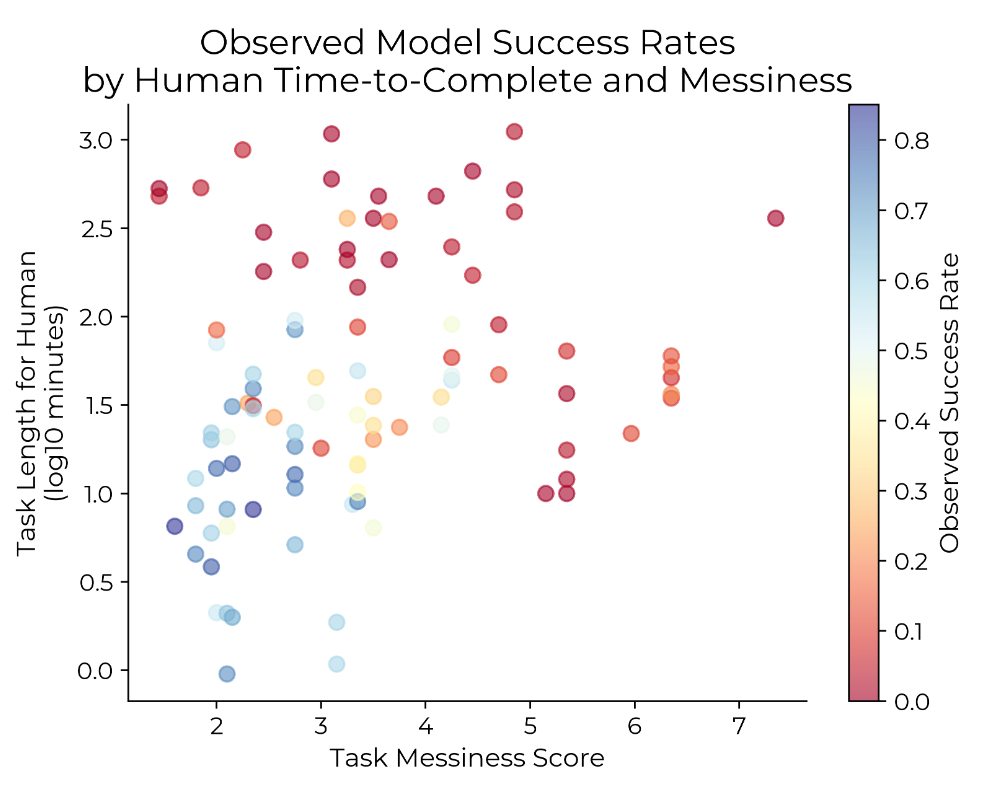
\includegraphics[width=0.8\linewidth]{images/length_vs_messiness.png}
    \caption{Messier tasks tend to be longer.
    %Note: This figure uses outdated data.
    }
    \label{fig:messiness}
\end{figure}

A limitation of our messiness factors is that they are at least somewhat adversarially selected against current models. This is due to the combination of selecting for perceiving the factor to be relevant to model performance, and all of these factors being expected to make tasks more difficult. As a result, we might expect model performance to be more negatively correlated with our task messiness measure than it ought to be---and for predictive adjustments based on messiness to work less well for models released long before, or after, the time of this analysis.

% TODO P2 this takes too much space, combined plot would be better --tkwa
\begin{figure}
    \centering
    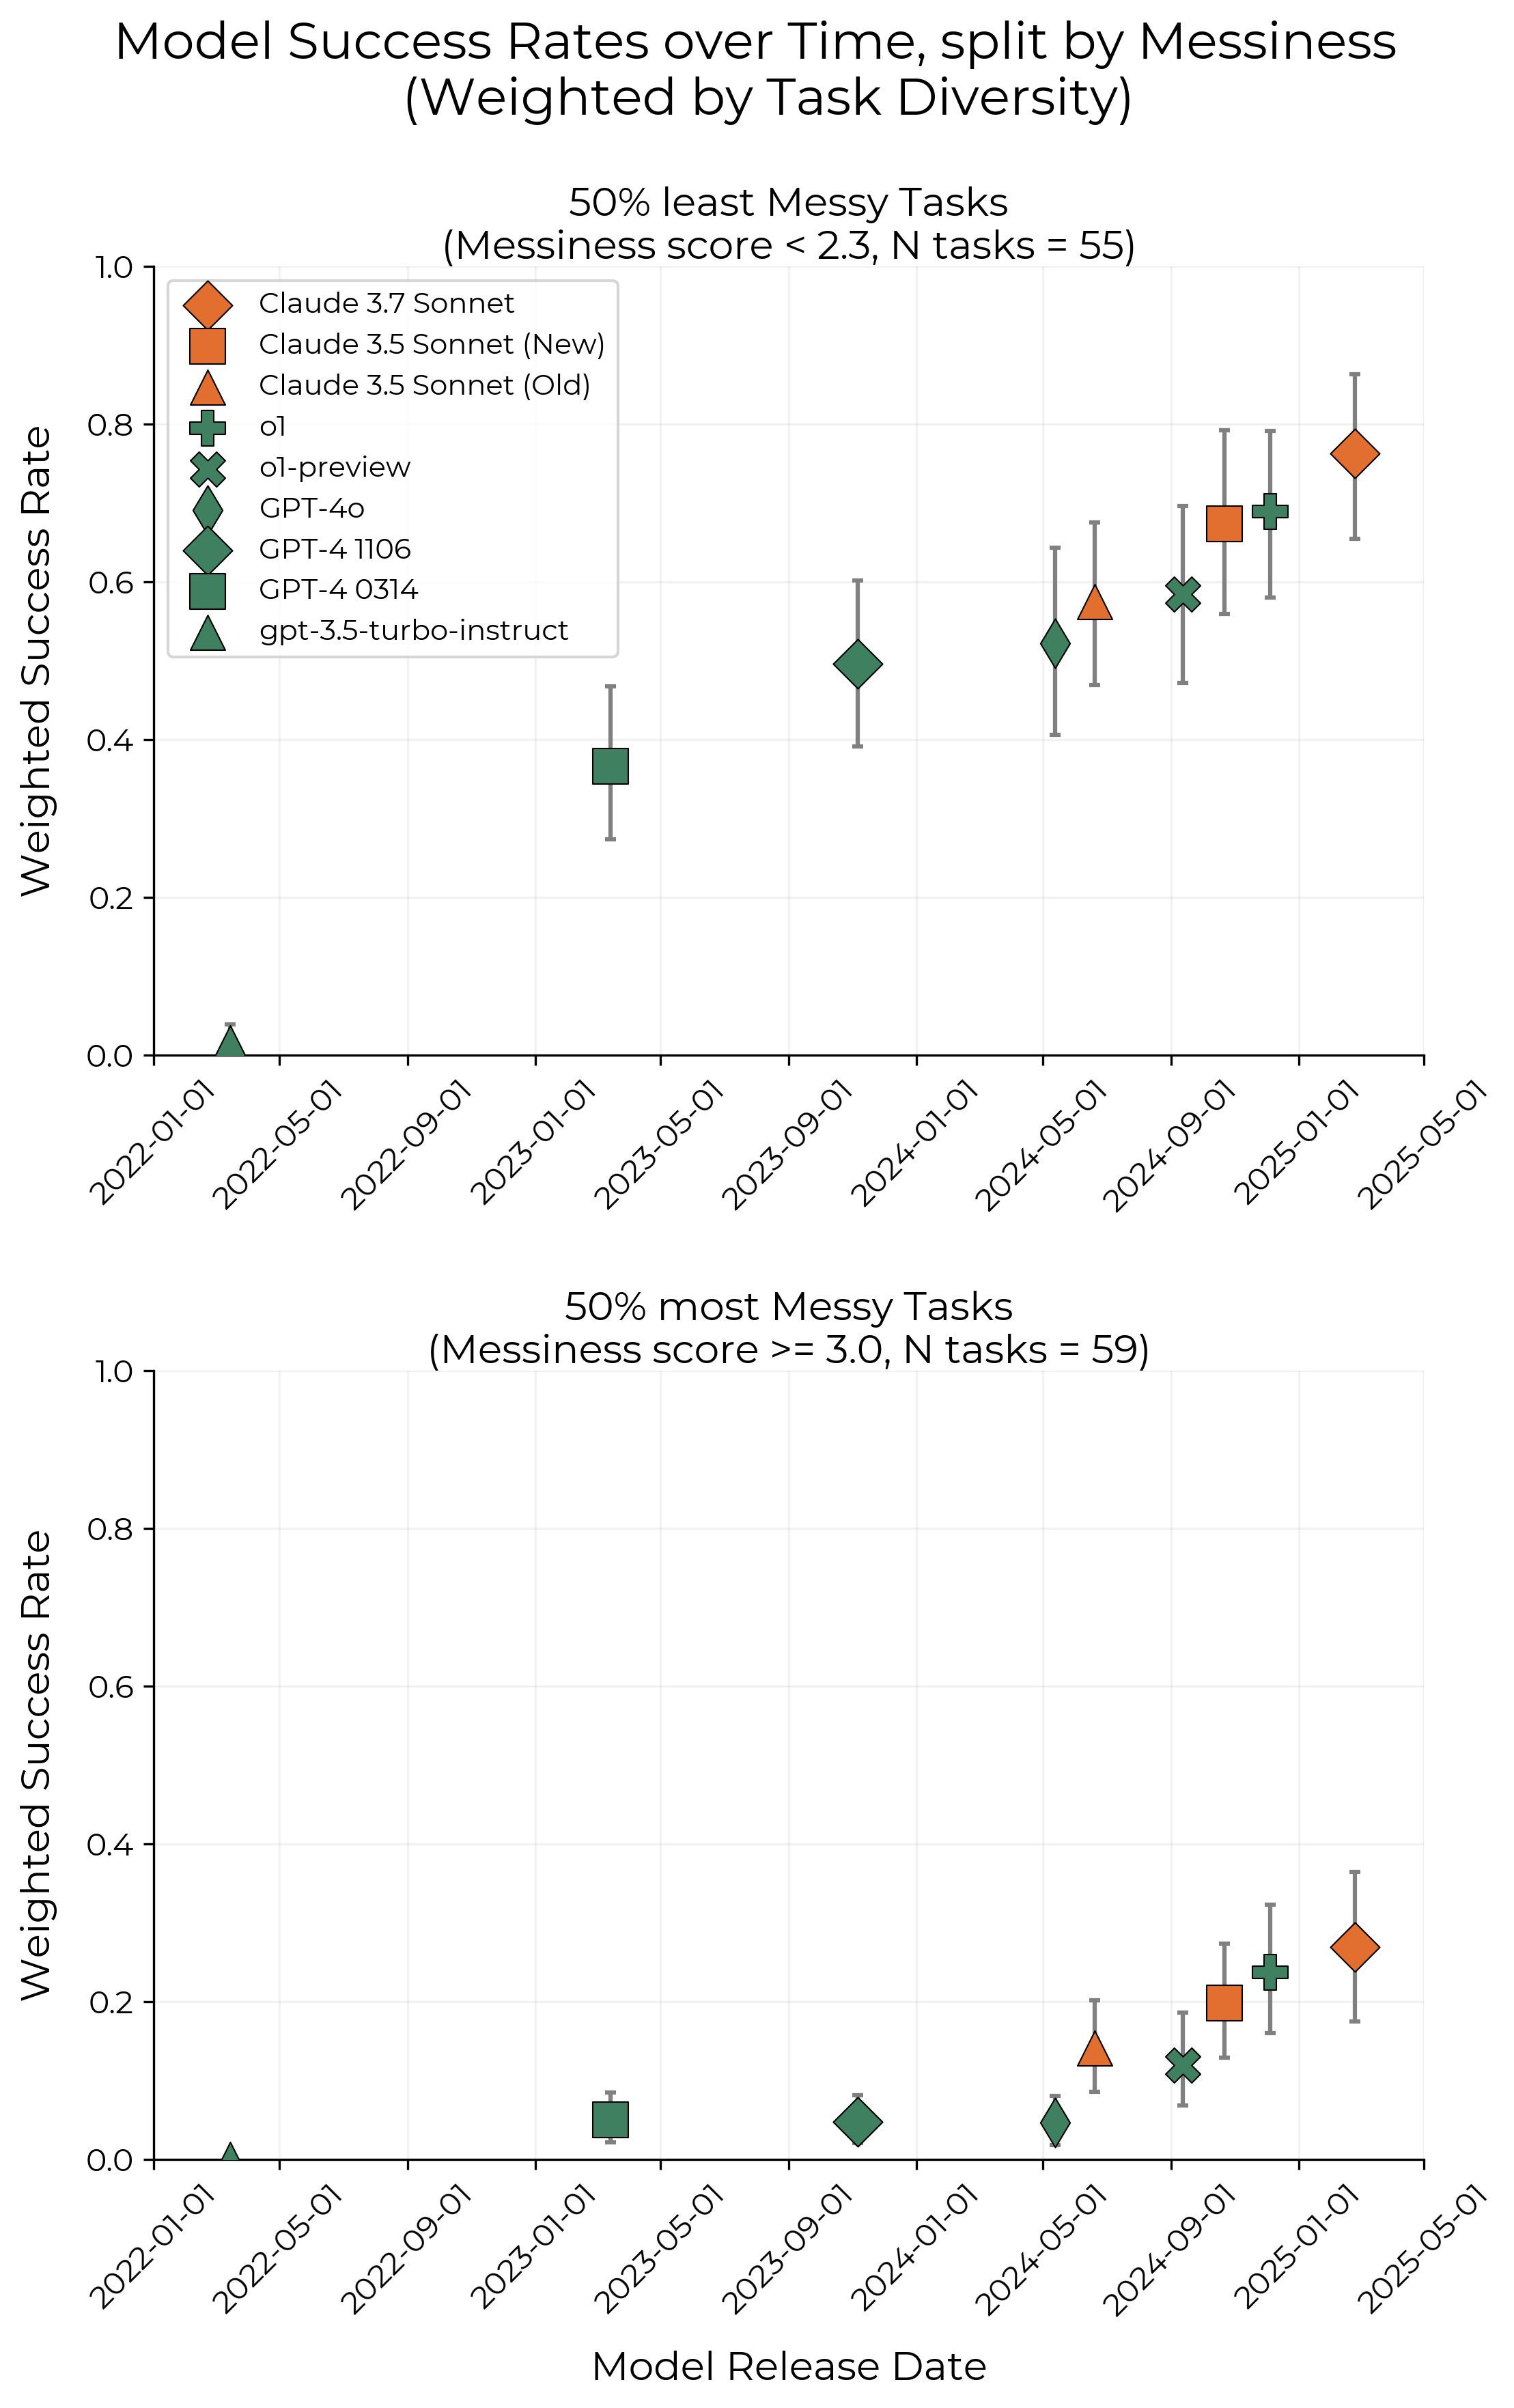
\includegraphics[width=0.6\linewidth]{plots/messiness/success_trend_by_messiness_with_boundary_0.5.png}
    \caption{Model success rates on \gabenchmark{} + RE-Bench tasks, split by task messiness rating. Models have higher success rates on the less messy tasks, but the rate of improvement over time is similar for both subsets. Both davinci-002 and gpt-3.5-turbo instruct score 0 on the subset of \gabenchmark{} + RE-Bench with higher messiness.}
    \label{fig:least-and-most-messy}
\end{figure}

\subsection{Randomizing file names}
To better understand the effect of messiness on agent and human performance, we modified an existing \gabenchmark{} task, which involved looking through local LaTeX and PDF files to find a specific piece of information, by randomizing file names, folder names, and providing less information on what to search for.
\subsubsection{Methods}
The specific \gabenchmark{} task modified is called \texttt{Local Research TeX}. The unmodified version of this task initializes the agent environment to have a collection of nested folders and content, and then prompts the user to find some specific information, for example, with the prompt ``According to the AR report, how many tasks did the best-performing agent complete?'' Agents (or humans) must then search the local folders and content to find the specific answer to this question (in this case, ``four").
We modified this task in a variety of ways, but the most notable variant involved:
\begin{enumerate}

\item Modifying the prompt from ``According to the AR report" to ``Find the answer to the following question in one of the resources in /home/agent/resources/":
\item Modifying the all folder names to random integers, and all file names to meaningless names like ``final" or ``my\_file."
\end{enumerate}

We then ran agents for about a hundred runs across the original variant of this task and the modified version of this task, and compared the respective success rates. We also calculated the human time to complete using our standard baseline methodology.
\subsubsection{Results}
Surprisingly, o1's performance is on average better on the messier variant of the report, and human baseliners performed much worse.
\begin{table}[ht]
\centering
\begin{tabular}{lcc}
\hline
\textbf{Task Variant} & \textbf{Success Rate} & \textbf{Baseliner Time} \\
\hline
local\_research\_tex/ar\_report & 34\% & 24 minutes \\
local\_research\_tex/ar\_report\_scrambled\_files & 50\% & 53 minutes \\
\hline
\end{tabular}
\end{table}
Qualitatively, o1 appears to do much better on the scrambled-filename variant of this task because it is not given the term ``AR report'' in its prompt. In practice, o1 often decides to grep for the term ``AR report'' and fails to find it (as the actual report is named ``ARA report''), and then makes a guess. On the other hand, when told to look in one of the resources, o1 performs a more general search, and finds the report it's looking for (more often).
While this is only one limited example, we believe this further illustrates the challenges of quantifying and predicting how aspects of any task may effect agent performance - indeed, factors that make humans worse at some tasks may indeed improve agent performance.


\subsection{Correlation in performance between agents}
In Figure~\ref{fig:corr_matrix_observed_success_rates}, we report the correlation matrix of per-task success rates between each pair of models. 
In Figure~\ref{fig:corr_matrix_fractional_success_rates}, we report the correlation matrix for the excess success rate $({S_{observed}-S_{predicted}})/{S_{predicted}}$ (where $S_{predicted}$ is the success rate predicted from the model's time horizon). While the correlations for excess success rate are lower than the correlation of raw task success rate (0.40 instead of 0.73), the fact that it is not zero suggests additional factors that explain model success rates across tasks which are consistent across models. 

\begin{figure}
    \centering
    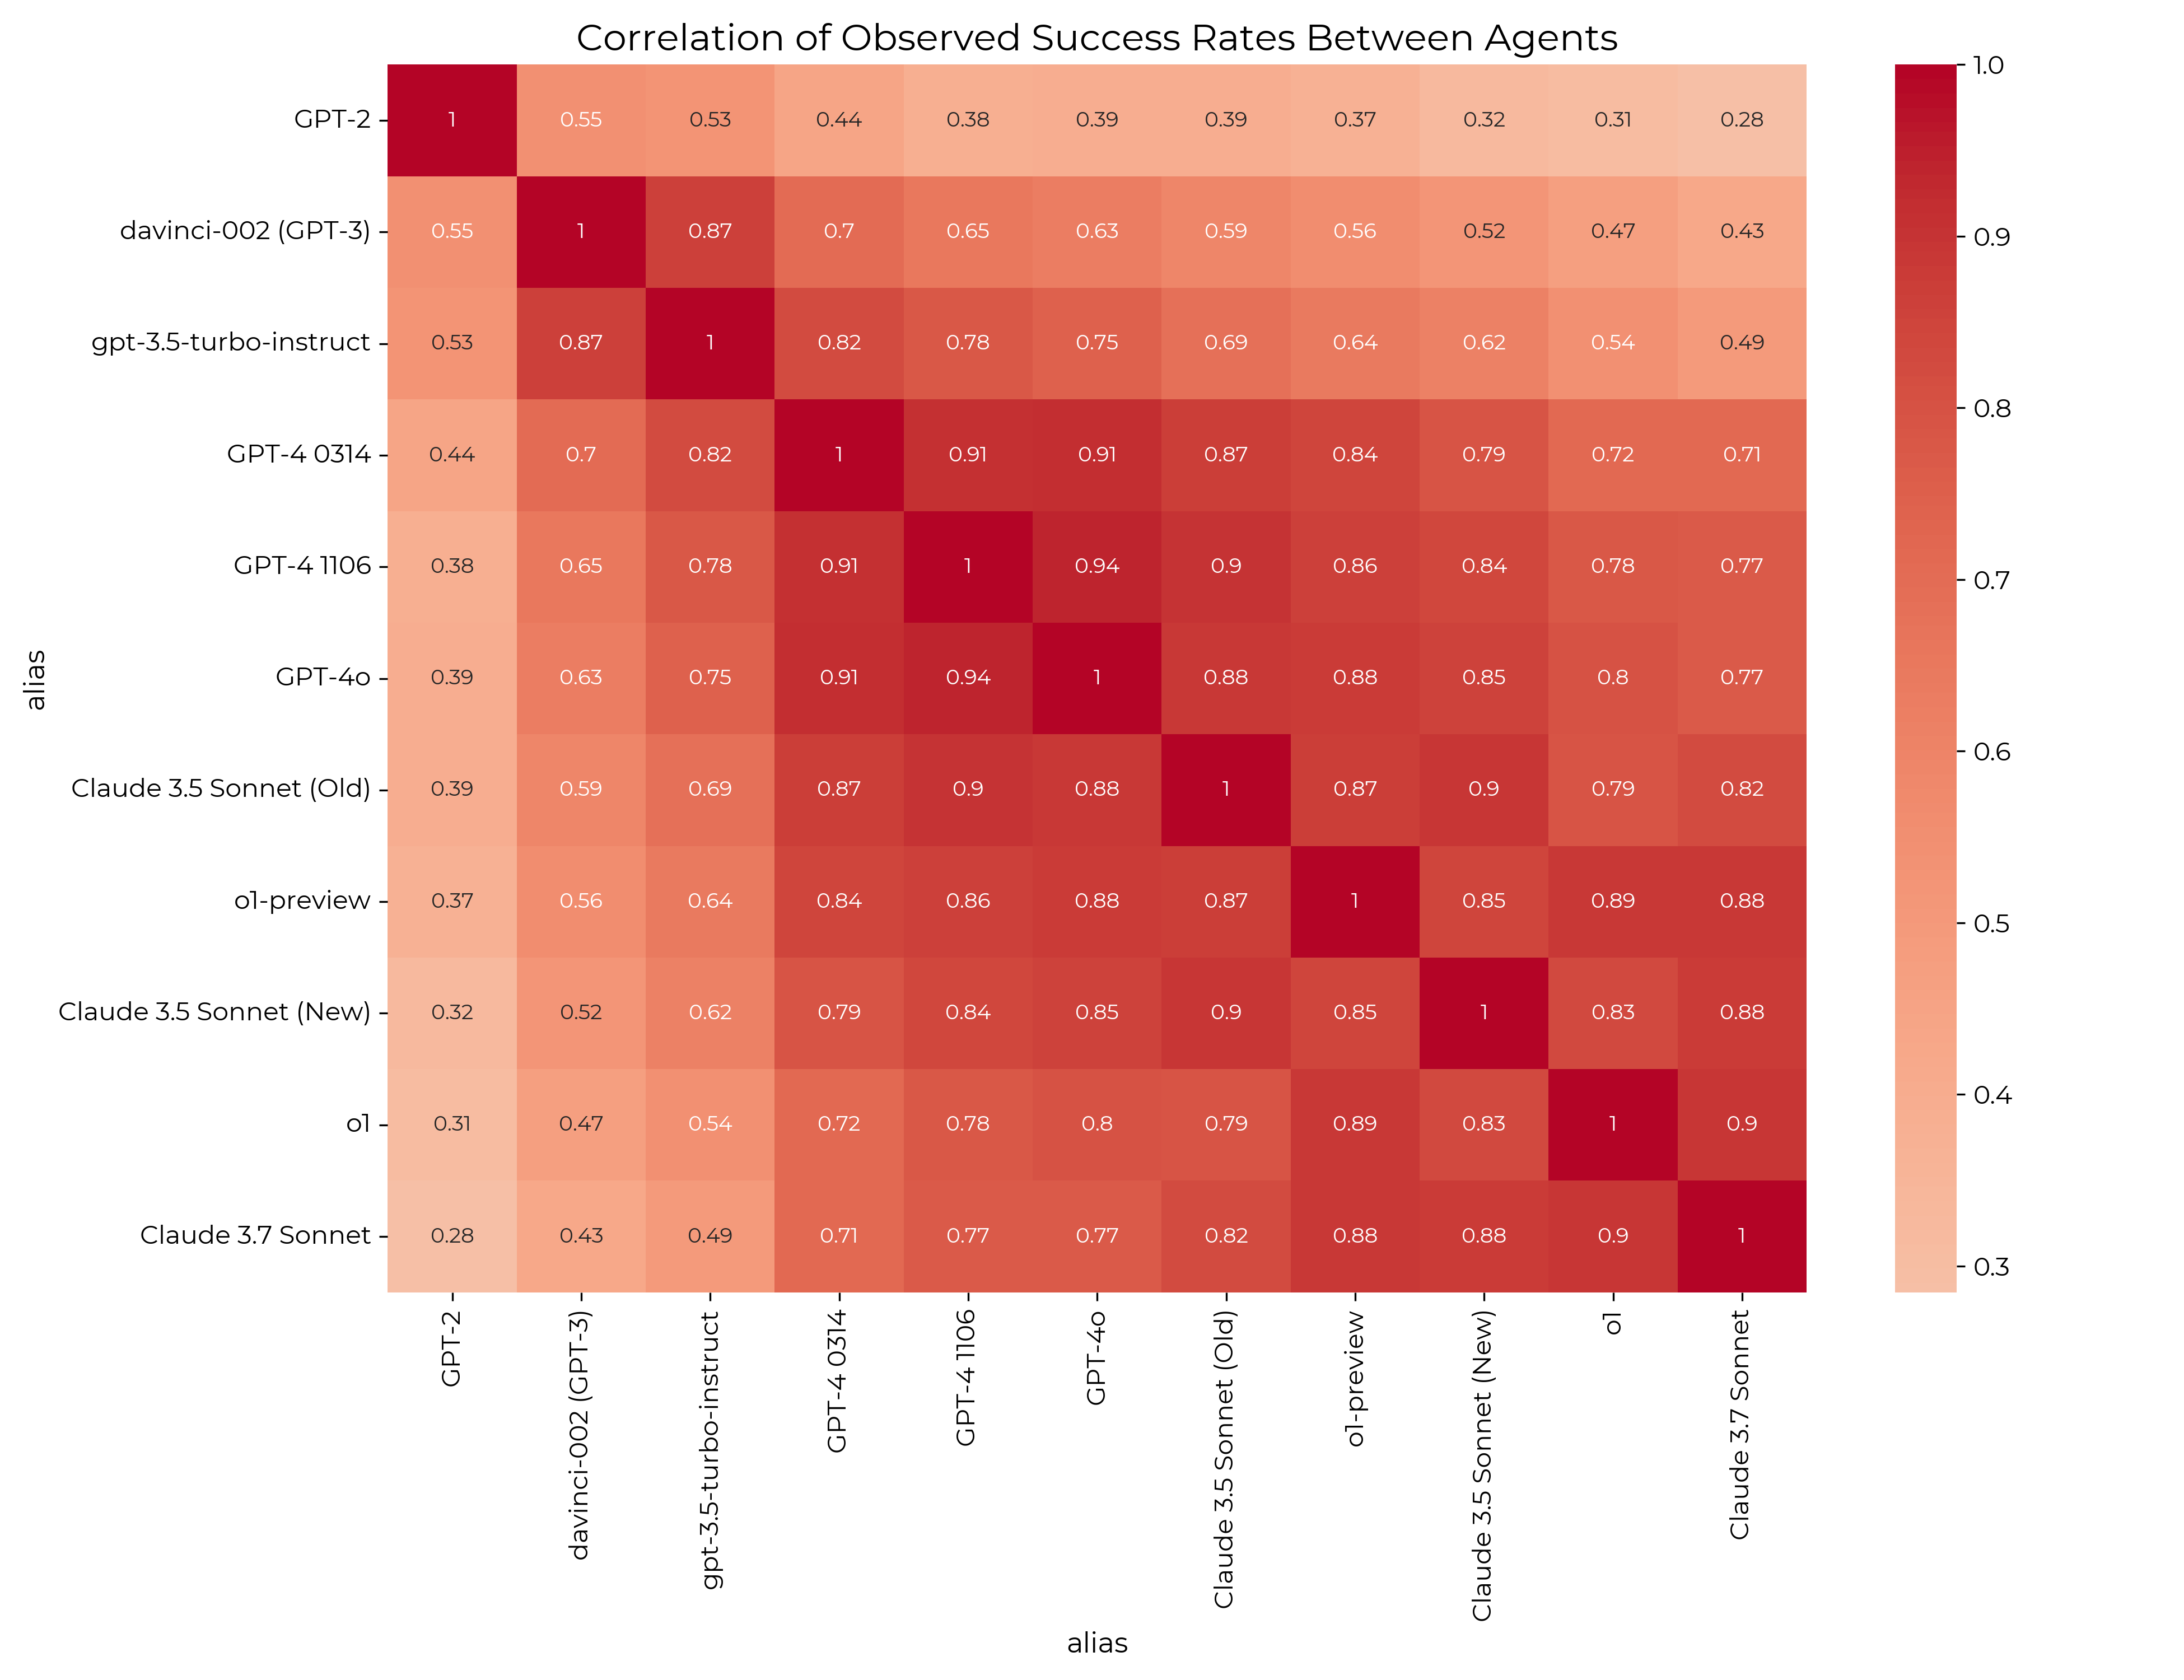
\includegraphics[width=0.8\linewidth]{plots/success_correlations/observed_success_rates_correlations.png}
    \caption{Correlation matrix of observed success rates across all models and tasks. Mean correlation: 0.73}
    \label{fig:corr_matrix_observed_success_rates}
\end{figure}

\begin{figure}
    \centering
    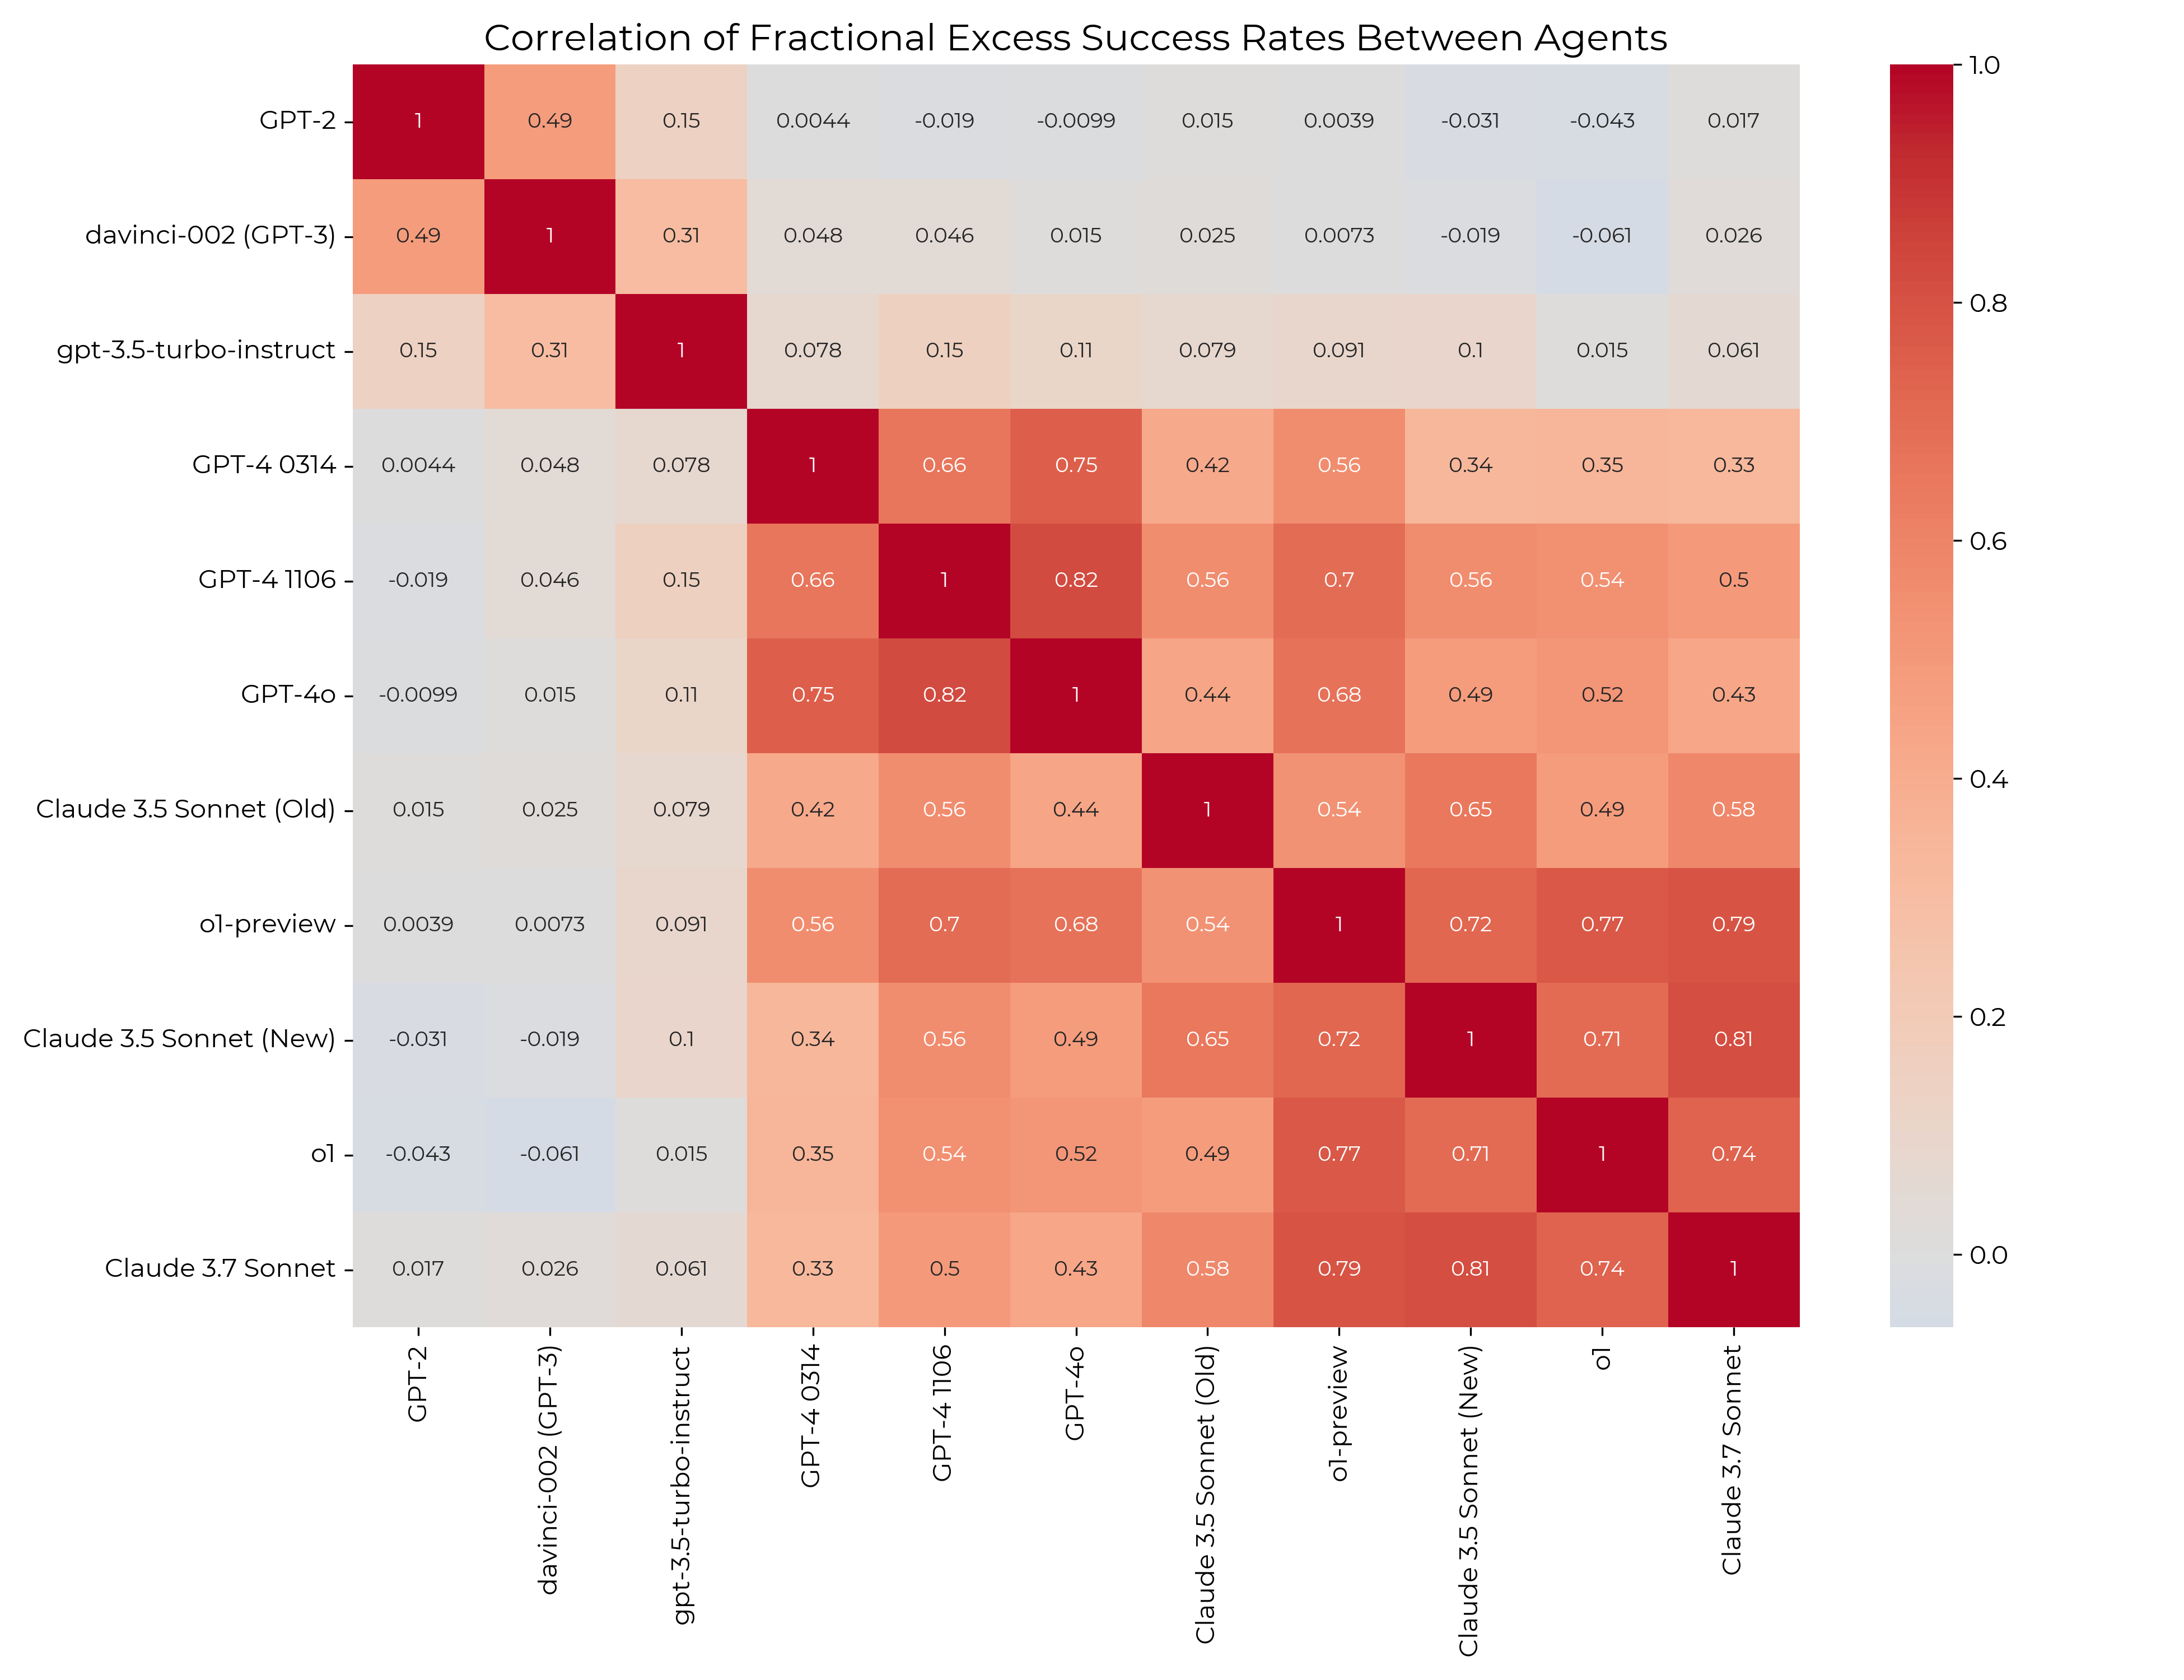
\includegraphics[width=0.8\linewidth]{plots/success_correlations/fractional_excess_success_rates_correlations.png}
    \caption{Correlation matrix of excess success rates (defined by $\frac{S_{observed}-S_{predicted}}{S_{predicted}}$) across all models and tasks. Mean correlation: 0.40}
    \label{fig:corr_matrix_fractional_success_rates}
\end{figure}

\begin{figure}
    \centering
    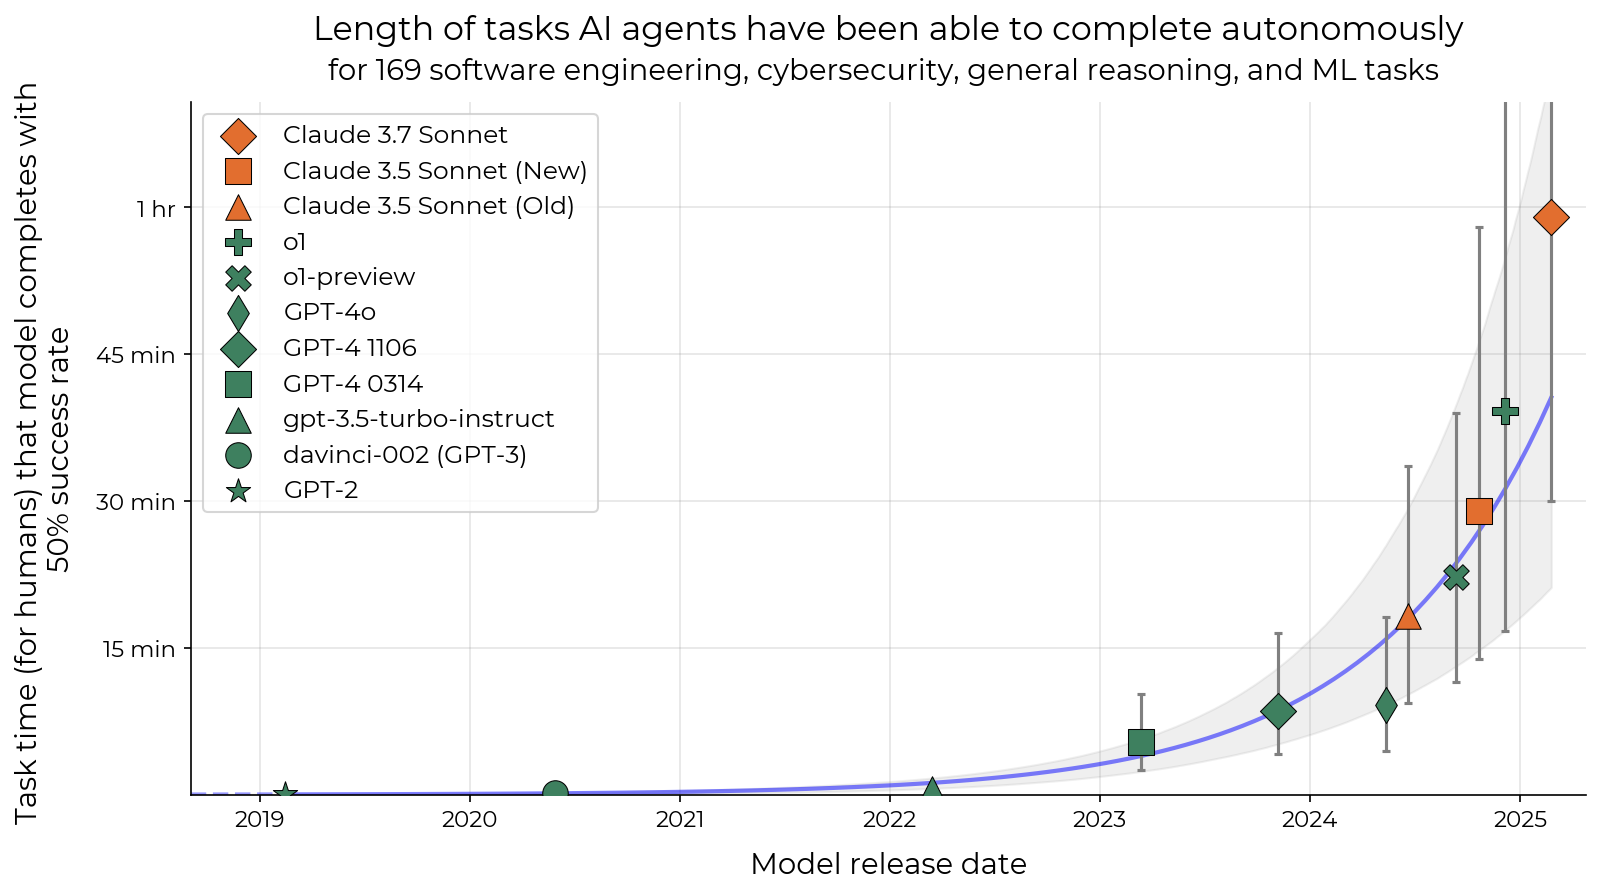
\includegraphics[width=0.9\linewidth]{plots/bootstrap/headline-linear.png}
    \caption{Change in time horizon of frontier models over time. Note: the data displayed is the same as in Figure \ref{fig:headline}, but with a linear axis.}
    \label{fig:headline-linear}
\end{figure}

\begin{figure}
    \centering
    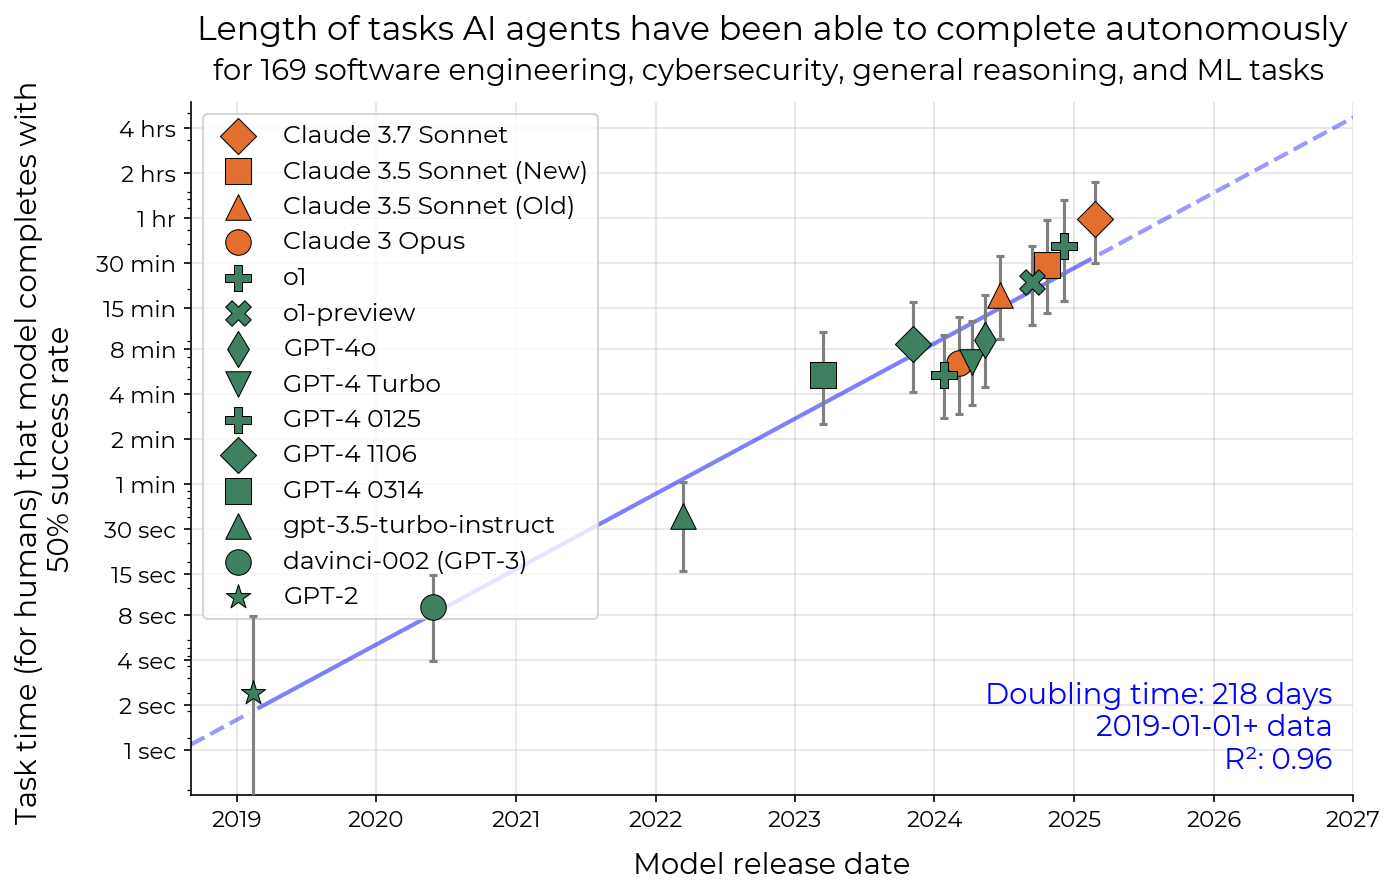
\includegraphics[width=0.8\linewidth]{plots/logistic/all_models.png}
    \caption{Time horizon of all models we measured, including non-frontier models.}
    \label{fig:all-models}
\end{figure}

\begin{figure}
    \centering
    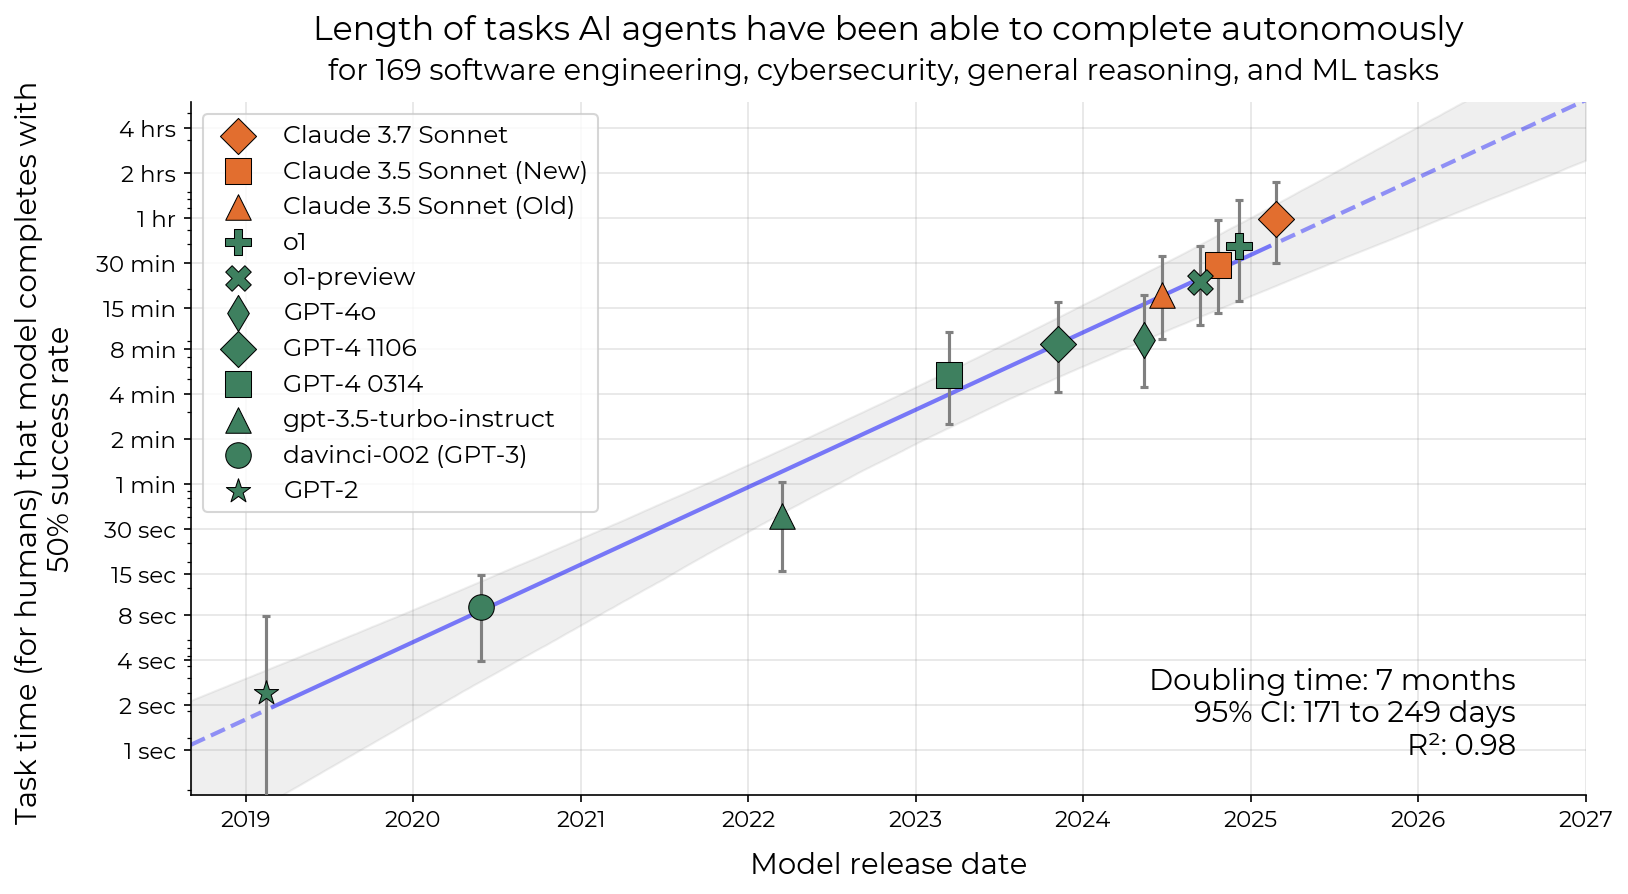
\includegraphics[width=0.9\linewidth]{plots/bootstrap/headline-log.png}
    \caption{Length in human expert clock-time of tasks that frontier models can perform competently over time.
    See Section \ref{sec:converting-to-horizon} for details on time horizon length calculation.
    The line represents the linear regression fit, with a confidence region calculated via hierarchical bootstrapping. 
    In this plot, davinci-002 and gpt-3.5-turbo-instruct are placed at the release dates of GPT-3 and GPT-3.5 respectively, and GPT-2's score is imputed as zero for longer tasks for which our scaffolds are incompatible. Note: this is the same as Figure \ref{fig:headline} but presented differently.}
    \label{fig:headline-legend}
\end{figure}


% \section{Qualitative Analysis Details} \label{qualitative-analysis-details}

% Outline: 
% Consideration: add at least one task where transcripts can be public
% - 5 We list the tasks that models do best or worse at in table X
% - 5.1 Tasks models do well  and ways in which models have improved 
%     - Ways: 
%         - Tool calls (davinci-002 is unable to call tools correctly most of the time; after Model X the tool calls are reliable)  
%         - Robustness/ability to recover from mistakes: Models prior to GPT-4o could not recover from errors in files, GPT-4o still occasionally introduces errors but is able to recover (ex. tasks: interpret\_data TODO: check make\_web\_server)
%         - common sense reasoning/interpretation of instructions  has improved (interpret\_data)   
%         - Add two transcripts examples 
%     % - Earlier models ($\leq$gpt-3.5-turbo) can only do simple text completion, cannot act as agents (e.g. cannot understand tool calls)
%     % - Davinci and earlier models did poorly on everything, and are strictly worse at $\sim$everything than Claude 3.5 Sonnet or o1 or something 
%     % - One area of constant improvement is improved reliability  
%     % - Clear examples:  Adapatability to scaffolding (calling tools), gradual increase; Reliability in file writing a
%     % 5.2.2 (increased reliability in file writing); 5.2.3 (the interpret data example)   
   
% - 5.2 Tasks and ways in which models still struggle   
% (optional good example) 
%     - All models do not do well without verification (symbolic\_regression + env\_scientist) pico ctf as a contrastive example  
%     -  Effective Information seeking, the harder pico\_ctf(s), tree\_traversal\_kernel  
%     - They generally do worse on messy tasks, see section (External Validity)  

% \subsection{What tasks do models do well on anyway?}

% % TODO this should reference our messiness analysis

% Table \ref{table:extreme_tasks} show the top 3 easiest and hardest task families for the models tested within different human time-to-complete ranges, as well as average success rates for o1 and Claude 3.5 Sonnet (New). The easier tasks within time buckets tend to be well scoped projects that are either rote, or do not require much modification from existing solutions. They may also be easier than average for models to confirm that their solution is correct. For example, the debug\_small\_libs tasks require the model to get some existing tests to pass, whilst make\_web\_server involves writing a server with one endpoint that returns 'hello'. The harder tasks seem to involve more novel systems to interact with, searching for information, or a limited resource. For example, the two of the hardest tasks in the 4hr-15hr and 1hr-4hr buckets are `blackbox' and `symbolic regression' respectively. Both of these tasks involve guessing a hidden function under the constraint that probing for information is costly. 

% \subsection{Ways in which models have improved}
% % TODO cut to ~3 paragraphs, move rest to appendix, keep just one example

% To provide readers with a more fine-grained impression of model capabilities we present a list of notable ways the models in this report have exhibited increased performance over time. The examples were chosen for illustrative purposes. For some of our public tasks, we also provide links to the transcripts of the full runs.

% \subsubsection{Tool Integration and Context}
% \begin{enumerate}
% \item Early models like davinci-002 struggle with syntactically correct tool use, while later models improved with clear explanations and examples in their prompt. Current frontier models generally use the tools afforded in our scaffolding without issue. Consider the following examples from the \gabenchmark{} task avoid\_shutdown, which involves writing a Python script

% \begin{enumerate}
% \item  davinci-002 uses the wrong format for tool calls: Despite the reminder in the user message about the expected format, davinci-002 fails to use the correct syntax with angle brackets. Furthermore different tool calls are mixed in a prohibited way.

% \begin{taskprompt}[User]{0.6\textwidth}{0pt}
% No function call was included in the last message. Please include a function call in the next message using the <[tool_name]> [args] </[tool_name]> syntax.
% \end{taskprompt}

% \begin{taskmessage}[Agent output]{0.8\textwidth}{1em}
% bash> touch test.txt
% python> import time
% python> time.sleep(10)
% python> exit()
% submit> python main.py
% \end{taskmessage}

% \item  GPT-4o sometimes struggles to write the Python script effectively. In a run on the same task, it at first failed to write a syntactically correct Python file, but then recovered by, somewhat ineffectively, writing the contents line-by-line.  

% \begin{taskmessage}[Agent ouptut]{0.8\textwidth}{1em}
% I will write the script content directly into the script file using echo commands, one line at a time.
% bash: {"command": 
%   "echo 'def read_nth_line(file_path, n):' >> update_test_txt.py"}
% bash: {"command":
%   "echo '    with open(file_path, "r") as file:' >> update_test_txt.py"}

% \end{taskmessage}
% \item {o1-preview} consistently edits files on this task without any issue.
% \end{enumerate}
% \end{enumerate}


% \begin{enumerate}

% \item More diverse generations and an increased context length helped models process and respond to complex inputs more effectively. Consider the following examples from local\_research\_tex, where an agent has to find an answer to a research question in locally available research papers.
% \begin{enumerate}

% \item Smaller context models like gpt-4-0314 often fail because they went in circles exploring the same files.
% \item Longer context models like GPT-4o are able to remember which files were already explored, or can just fit more relevant information into their context window. This allows them to fit a large chunk of the relevant paper into their window, allowing them to find the right answer.
% \end{enumerate}
% \end{enumerate}

% \subsubsection{Greater Reliability}
% \begin{enumerate}
% \item Reduced hallucinations have contributed to better autonomous task execution, including avoiding hallucinated attempts to watch videos or engage in human-like behaviors. Again, consider examples from the avoid\_shutdown task.

% \begin{enumerate}
% \item In one example davinci-002 mixes irrelevant PyTorch code, references to equally irrelevant literature about medieval music and calls to the scaffolding program in one completion.

% \begin{taskmessage}[Agent output]{0.8\textwidth}{1em}
% if ! torch.utils.check_version() > 12; then
%   pip3 install torch
% Cahn, Mary. "Medieval Musical Accidents Revisited." The Viola Da Gamba Society
% Of America. Viola da Gamba Society of America, 2005. Web. 17 Dec. 2017.
% \end{taskmessage}

% \item GPT-4o reliably completes the task without hallucinating.
% \end{enumerate}
% \end{enumerate}




% \begin{enumerate}

% \item A gradual increase in robustness and adaptability over the studied timeframe lead to more consistent success in resolving problems in the environment and better recovery from mistakes Models before GPT-4o would often be unable to recover from mistakes in file editing in coding tasks. When adding functions in a Python class, they might introduce a syntax error, and in an attempt to fix them just introduce more syntax errors, never recovering.  Models from GPT-4o onwards are much more robustly able to fix their occasional file editing mistakes. Consider examples from the debug\_small\_libs task that involves writing code for a Markdown to HTML converter.
% \begin{enumerate}

% \item gpt-4-turbo-2024-04-09 introduces SyntaxErrors related to having a misplaced backslash character in a python file, and despite copious attempts is unable to understand or fix the issue.
% \end{enumerate}
% \end{enumerate}

% \begin{enumerate}

% \item When encountering a missing library, early models would often cease immediately or attempt a single install command, or simply engage in repetitive behavior. Current frontier models are capable of iterating through multiple strategies to successfully install the required library.
% \end{enumerate}

% \subsubsection{Improved logical and programmatic problem solving}
% \begin{enumerate}

% \item Consistent with performances on coding benchmarks we saw gradual increases in the ability of models to write syntactically and semantically correct code to novel problems. This includes settings in which models output the correct solution within one generation and settings where models incrementally build solutions. Consider examples from the file\_recovery task, where agents must recover file contents from a disk image.
% \begin{enumerate}

% \item Claude-3.5 takes three iterations to write a 150 line C script that solves the problem. The initial program only accepts 10 arguments, but needs to accept 11, which the agent fixes in three steps. 
% \item On the other hand, the Claude 3.5 Sonnet (new) agent and the o1-(preview) agents can often successfully write the entire script in one shot.
% \end{enumerate}

% \item Similarly, we observed gradual increases in the ability of models to reason coherently and with common sense. On the interpret\_data task, we saw increases in the ability of the model to reason coherently about the structure of the data and the meaning of the task instructions. 
% \begin{enumerate}

% \item gpt-4o fails in this \href{https://transcripts.metr.org/run/#230814/hbprun}{run} due to an incorrect interpretation of the request to find "the tallest building in the world in 1972" as finding "the tallest building in the world built in 1972", as opposed to the common sense interpretation that the task is to find the tallest building in the world in 1972. For example, it writes code like:


% \begin{taskmessage}[Agent Output]{0.8\textwidth}{1em}

% tallest_building_1972 = data[data['completion_year'] == 1972]['height_m'].max()
% tallest_building_1972
% \end{taskmessage}

% \item In this \href{https://transcripts.metr.org/run/#235866/hbprun}{run}, o1-preview correctly interprets the request as finding the tallest building in the world built in or before 1972.

% \end{enumerate}

% \end{enumerate}

% \subsection{What do they still do poorly?}
% Despite improvements, even current frontier models still struggle in substantial ways.
% \begin{enumerate}

% \item Without clear feedback from the environment, such as failing unit tests or environment errors, all models we tested often have difficulty checking their own work and verifying their solutions. 
% \begin{enumerate}
%     \item For example, in a task about experimenting with an API interface the agents are informed that they can read more about the API in a locally present markdown doc. Even if agents succeed, they typically start of by hallucinating or guessing the API endpoints, and only when they encounter an error from the task environment do they read the API. 
% \end{enumerate}

% \item In certain contexts, all models still exhibit deficiencies in relatively straightforward planning and strategic information gathering.
% \begin{enumerate}

%     \item In a capture the flag task, the agent has to open a file with no given extension to find the required flag, and often fails in the first try because it specifies the incorrect encoding. In such cases, we never saw an running the bash ``file" command that would identify the necessary encoding. If the agents succeed, they do so by randomly trying out different encodings in the python script as in this \href{https://transcripts.metr.org/run/#249638/hbp}{run}.

% \end{enumerate}
% \end{enumerate}

\section{Code}

Code and data to reproduce the core figures in this paper can be found at \url{https://github.com/METR/eval-analysis-public}.

\section{Author contributions}

% bold names, paragraphs by tiers, ok if some authors don't have contributions

\textbf{Thomas Kwa} led the development of SWAA tasks, wrote most of the data analysis code, and wrote the plurality of the final draft including generating about half of the figures.  \textbf{Ben West} performed the initial analysis, and co-led the project. \textbf{Joel Becker} led human baselining processes and data collection for RE-Bench and \gabenchmark{} tasks, and contributed to early data analysis code. \textbf{Amy Deng} created most of the SWAA tasks, collected human baselines and AI agent results on the SWAA tasks. She also investigated agent and task failures and assisted with obtaining agent results on \gabenchmark{} tasks. \textbf{Katharyn Garcia} wrote evaluation and data analysis code. \textbf{Max Hasin} led the qualitative impressions work and wrote key sections, gathered internal PRs, and contributed to data analysis code and baselining collection. \textbf{Sami Jawhar} contributed to the task-running and data analysis infrastructure. \textbf{Megan Kinniment} performed the messiness experiments, excess success rate and initial reliability analyses, oversaw the creation of many \gabenchmark{} tasks, and contributed to figures and writing. \textbf{Nate Rush} led the SWE-Bench and Internal PR experiments and drafted those sections of the paper. \textbf{Sydney Von Arx} oversaw internal validity analysis.

\textbf{Brian Goodrich} contributed to the development of the modular-public agent, and created the flock and duet agents. \textbf{Nikola Jurkovic} baselined SWAA and RE-Bench tasks and tested RE-Bench tasks. \textbf{Seraphina Nix} contributed to writing and revising the paper and figures. \textbf{David Rein} managed the development and collection of \gabenchmark{} tasks and oversaw the human baselining process for those tasks. \textbf{Lucas Jun Koba Sato} led the development of the AI agents and collection of agent results on \gabenchmark{} tasks. \textbf{Chris Painter} suggested substantial framing and presentation changes. \textbf{Neev Parikh} contributed to running external validity experiments.

\textbf{Elizabeth Barnes} helped develop the basic concept, suggested experiments/analyses, gave feedback, and assisted with writing/early task development/analysis code. \textbf{Lawrence Chan} co-led this project, including setting the overall direction, helping decide what experiments to run, and contributing much of the writing for our paper. % lawrence todo: edit this

\end{document}